\documentclass
[
    paper = a4,
    pagesize,
    12 pt,
    oneside,                       % Chose ›oneside‹ for digital version, ›twoside‹ for printed version.
    open = right,
    DIV = calc,
    BCOR = 0 mm,                   % Binding correction. Only necessary for printed version. Depends on actual binding.
    bibtotoc
]
{scrbook}

% Do not change the following commands.
\newcommand*{\printTitle}{}
\newcommand*{\printAuthor}{}
\newcommand*{\printDateOfBirth}{}
\newcommand*{\printPlaceOfBirth}{}
\newcommand*{\printSubject}{}
\newcommand*{\myTitle}[1]{\renewcommand*{\printTitle}{#1}}
\newcommand*{\myName}[1]{\renewcommand*{\printAuthor}{#1}}
\newcommand*{\myDateOfBirth}[1]{\renewcommand*{\printDateOfBirth}{#1}}
\newcommand*{\myPlaceOfBirth}[1]{\renewcommand*{\printPlaceOfBirth}{#1}}
\newcommand*{\mySubject}[1]{\renewcommand*{\printSubject}{#1}}

\myTitle{Visualizing Shortest Path Algorithms on Tiled Map Data}  % Change!
\myName{Julius Milian Severin}  % Change!
\myDateOfBirth{March~12, 1995}  % Change!
\myPlaceOfBirth{Berlin, Germany}  % Change!
\mySubject{{Graph Algorithms}{Visualization}}  % Change!
\advisorOne{Martin~S. Krejca}
\advisorTwo{Thomas Bl\"asius}
\myGermanTitle{Visualisierung von K\"urzeste-Wege-Algorithmen auf segmentierten Karten}

\usepackage[utf8]{inputenc}
\usepackage[T1]{fontenc}
\usepackage[english]{babel}

\usepackage{graphicx}

\graphicspath{{Images/}}

\usepackage{pgf}

\usepackage							% Microtypography tuning.
[
	protrusion = true,
	expansion = false,
	tracking = true,
	kerning = true,
	spacing = false,
	babel = true
]
{microtype}							% http://ctan.mirrorcatalogs.com/macros/latex/contrib/microtype/microtype.pdf

\SetTracking[unit = space]{font = */*/*/sc/*}{25}   % Adjust kerning for small caps.

\SetExtraKerning[unit = space]		% Adjusted kerning for certain characters.
{
	font = */*/*/*/*
}
{
	: = {100, },
	; = {100, },
	? = {150, 150},
	! = {150, 150},
	: = {250, },
	; = {150, },
	? = {250, 250},
	! = {250, 250},
	» = { , -200},
	« = {-200, },
	› = { , -200},
	‹ = {-200, },
	– = {200, 250},
	— = {200, 250},
	@ = {200, 200}
}

\usepackage{booktabs}
\usepackage{breakurl}
\usepackage{emptypage}

\usepackage[bottom]{footmisc}
\usepackage{remreset}

\makeatletter
    \@removefromreset{footnote}{chapter}
\makeatother

\renewcommand*{\footnoterule}{\rule{0 pt}{0 pt}}
\deffootnote[1.2 em]{1.2 em}{0 em}{\makebox[1.4 em][l]{\textbf{\thefootnotemark}}}

\usepackage{xparse}

\DeclareDocumentCommand{\myfootnote}{o o o m}
{%
    \IfNoValueTF{#1}%
    {%
        \footnote{#4}%
    }%
    {%
        \IfNoValueTF{#2}%
        {%
            \kern #1 em\footnote{#4}%
        }%
        {%
            \IfNoValueTF{#3}%
            {%
                \kern #1 em\footnote{#4}\kern #2 em%
            }%
            {%
                \kern #1 em\footnote[#3]{#4}\kern #2 em%
            }%
        }%
    }%
}

\usepackage{titlesec}

\titleformat{\chapter}
    {\normalfont\rmfamily\huge\bfseries}
    {\thechapter}{1 em}{}

\titleformat{\section}
    {\normalfont\rmfamily\Large\bfseries}
    {\thesection}{1 em}{}

\titleformat{\subsection}
    {\normalfont\rmfamily\large\bfseries}
    {\thesubsection}{1 em}{}

\titleformat{\subsubsection}
    {\normalfont\rmfamily\normalsize\bfseries}
    {\subsubsectionname}{1 em}{}


\pagestyle{headings}

\usepackage{amsmath}
\usepackage{amssymb}
\usepackage{amsfonts}
%\usepackage{upgreek}               % Use if you want to use upright lowercase and italic upercase greek letters.
%\usepackage{dsfont}                % Use if you want to use special symbols.

%\usepackage[printonlyused]{acronym} % Use if you want to have acronyms. http://mirror.hmc.edu/ctan/macros/latex/contrib/acronym/acronym.pdf

%\usepackage{pifont}				% Special symbols.
%\usepackage{fourier-orns}			% More special symbols.
\usepackage{lettrine}

\usepackage{enumitem}
\usepackage
[
	format = plain,
	textfont = {sf, footnotesize},
	labelfont = {sf, bf}
]
{caption}[2008/08/24]
\usepackage{subcaption}				% For using sub-figures.

\usepackage
[
    algo2e,
    ruled,
    vlined,
    linesnumbered,
    algochapter
]
{algorithm2e}

\SetAlCapFnt{\sffamily\footnotesize}
\SetAlCapNameFnt{\sffamily\footnotesize}

\usepackage[numbers]{natbib}

\makeatletter
    \def\NAT@spacechar{~}% NEW
\makeatother

\definecolor{darkblue}{rgb}{0, 0, 0.5}

\usepackage
[
	bookmarks = true,
	bookmarksopen = false,
	bookmarksnumbered = true,
	pdfstartpage = 1,
	pdftitle = {{\printTitle}},
	pdfauthor = {{\printAuthor}},
	pdfsubject = {{\printSubject}},
	backref = page,
	breaklinks = true,
	colorlinks = true,
	linkcolor = darkblue,
	anchorcolor = darkblue,
	citecolor = darkblue,
	filecolor = darkblue,
	menucolor = darkblue,
	pagecolor = darkblue,
	urlcolor = darkblue
]

\usepackage{hyperref}


\renewcommand*{\backref}[1]{}
\renewcommand*{\backrefalt}[4]
{
    \ifcase #1
        Not cited.
    \or
        \footnotesize (Cited on page #2.)
    \else
        \footnotesize (Cited on pages #2.)
    \fi
}

\usepackage{cleveref}

\begin{document}




\begin{document}


\frontmatter
% Title Page
\thispagestyle{empty}
\begin{center}
    {\Huge \textbf{\printTitle}}\\[7 ex]
    {\Large\textsc{Bachelor Thesis}}\\[4 ex]    
    {\large
        to attain the scientific degree\\[4 ex]
        \textbf{Bachelor of Science}
    }
    \vfill
    \includegraphics[width = 8 cm]{HPI_logo.pdf}\\[8 ex]
    \begin{tabular}{l}
        handed in by \textbf{\printAuthor}\\[1.1 ex]
        born \printDateOfBirth, in \printPlaceOfBirth\\[3 ex]
        \textbf{Advisor:} Prof.~Dr.~Tobias Friedrich\\[9 ex]
    \end{tabular}
    
    Potsdam, \today
\end{center}

% Abstract
\chapter*{}
\addcontentsline{toc}{chapter}{Abstract}
\thispagestyle{empty}

\begin{center}
    \large \textbf{Abstract}
\end{center}

Developing an algorithm is an iterative process.
Therefore an understanding of the different approches is important.
Furthermore, as the algorithm becomes more complex, it may come to different results than expected, when running on real data.

This thesis deals with those issues on the example of shortest path algorithm on tiled map data.
Therefore, multiple ways of visualizing a shortest path algorithm with respect of this specific class of algorithms are introduced.
Using those methods we were able to archieve a better understanding of the algorithms and built a powerful basis for discussions.
In addition we enabled the researchers to find the missbehaviour more easily.

\chapter*{}
\addcontentsline{toc}{chapter}{Zusammenfassung}
\thispagestyle{empty}

\begin{center}
    \large \textbf{Zusammenfassung}
\end{center}

Das Entwickeln eines Algorithmusses ist ein iterativer Prozess.
Daher ist es wichitg, dass alle Beteiligten, die verschiedenen Ansätze verstehen.
Ausserdem kann es mit wachsender Komplexität des Algoithmus dazu kommen, dass sich der Algorithmus auf echten Daten anders verhalten als gedacht.
Das finden der Ursache kann ein äußerst komplexes Verfahren sein.

In der folgenden Arbeit erklären wir, wie wir die Entwicklung eines Algorithmus zum finden kürzester Wege durch eine Visualisierung untersützt haben.
Dabei gehen wir auf die Probleme ein, die wir wärend der Entwicklung der Visualisierung lösen mussten.


% Table of Contents
\renewcommand*{\listfigurename}{\normalfont\rmfamily\Large\bfseries List of Figures}
\renewcommand*{\listtablename}{\normalfont\rmfamily\Large\bfseries List of Tables}
\pdfbookmark{\contentsname}{toc}
\microtypesetup{protrusion = false}
    \tableofcontents
    \begingroup
    \let\clearpage\relax
    \listoffigures                  % Comment out if necessary.
    \listoftables                   % Comment out if necessary.
    \endgroup
\microtypesetup{protrusion = true}


\mainmatter
\chapter{Introduction} \label{introduction}
% Algorithmen
Graphs are a common structure in computer science.
Therefore, developing more efficient graph algorithms plays a major role in algorithm engineering.

% Visualisierung
%During the process of development knowing how the algorithm behaves is really important.
During the process of development full awareness of all processes and changes in algorithm behaviour is necessary.
%As developing an algorithm is an iterative process it is fundamental to communicate about the different approaches and therefore create an understanding of them in the whole team.
As developing an algorithm is an iterative process it is of upmost importance that the research participants communicate constantly with respect to different approaches, and therefore maintain a high level of mutual awareness.
Furthermore, the developed algorithms can become quite complex and therefore the idea of how the algorithms should behave and the way they actually behave on real graph data, can diverge quite a lot.

% Projekt
In the twelve month, we developed a shortest-path algorithm on geographical tiled map data.
The tiles impact the algorithm insofar that the loading of a tile has high costs and should therefore be avoided as much as possible.
A tile needs to be loaded whenever one of its nodes is processed.
As the algorithm was developed for portable devices, it has access to the so-called cache: a fast storage medium.
The cache can store a limited amount of tiles.
Therefore, a tile only needs to be loaded whenever it is not in the cache.
Due to the limited size of the cache, loading a tile into the cache, requires removing another one, as soon as the cache is full.

As the human eyes are a fast way to access information, we decided to visualize the progress of the algorithm to achieve the necessary understanding.
Though there are many tools for visualizing graphs such as for example Walrus \cite{walrus}, and even multiple algorithm visualization tools such as VisuAlgo\cite{visualgo}, there is currently no visualization tool that fits our needs.
%This might result from the high amount of individual characteristics of our class of algorithms and its underlying graph.
One if the reasons might be due to the large amount of individual characteristics of our class of algorithms and its underlying graph.
Therefore, developing an new, self-created visualization that fits one's individual needs is necessary.

\paragraph{Outline.} We will be explaining different approaches we developed for visualizing the specific class of algorithms.
In \Cref{questions}, we will touch on different methods we created that may be used for displaying the algorithms.
In the following \Cref{main} those methods are then introduced, explained and discussed in more detail.
A discussion and outlook in \Cref{conclusion} concludes the thesis.


\chapter{Preliminaries} \label{questions}

In this chapter, we will first introduce the class of algorithms that the visualization will display.
Then, we will discuss the graph data the algorithms are running on.
Following that, the characteristics of the visualization are presented.
The implementation of those characteristics is then discussed in \Cref{main}.


\section{Problem Specification} \label{specification}

This section will present the scope the visualization is runnging in.
Therefore, in \Cref{framework} we are going to introduce the algorithms that are going to be displayed and in \Cref{spec_graph} the underlying graph is described.

\subsection{The Class of Algorithms} \label{framework}

The visualization we built has the purpose of visualizing shortest path algorithms.
A shortest path algorithm, in general, has the goal to find the path with the lowest summed weight from a given start node to a given target node in a weighted graph.

The class of algorithms is based on Dijkstra's algorithm\cite{DIJKSTRA1959} and its improvement, the A*-algorithm\cite{4082128}.
Dijkstra's algorithm commences at the start node from where it adds the neighbours of the node to a priority queue that sorts the elements according to their distance to the start node.
%proximity
In each iteration, the node with the highest priority (smallest distance) is removed from the queue and its neighbors are added to the queue, when not already inserted.
Whenever the node that is going to be removed from the queue is the target node, the shortest path is found.
This results in a uniformly spreading of the search space around the start node.

The A*-algorithm generally adopts this strategy.
Its goal is to search target oriented and therefore reduce the search space.
Therefore, the the A*-algorithm-queue is ordered not only by the summed distance of the edges to the start node but also by the linear distance to the target node.
Thereby, nodes presumably closer to the target get expanded first.
This leads to a target directed spreading.

At this stage, it is important to note that both algorithms create a coherent area of processed nodes.

\subsection{The graph} \label{spec_graph}

The underlying graph of the algorithms is a real-world road network.
Every node has given coordinates that refer to a certain position on Earth, the edges are directed and the weight of an edge can be calculated using its speed and its length.
What makes the graph special, is the fact that it is based on the Navigation Data Standard (NDS).
Based on the NDS the graph is split into tiles according to a geographical grid.

This impacts the algorithms in so far, that accessing tiles becomes the major effort on runtime, as the tiles are encrypted and compressed.
Hence, the algorithms should access as few tiles as possible.
As the algorithms are developed for portable devices, they have access to the so-called cache: a fast storage medium with limited size.
Since tiles can be stored in the cache, accessing a tile is only costly when it is not in the cache.
A tile is \emph{accessed} whenever one of its nodes is processed.
Due to the limited size of the cache, loading a tile into the cache requires removing another one, as soon as the cache is full.


\section{Basic Elements}

In \Cref{graph}, the representations of basic elements of the graph are introduced.
We discuss how to represent nodes, edges, and tiles in a meaningful way.
For the nodes, it is important to consider how they can be arranged on the screen, or rather discuss how to map the coordinates on the spherical Earth onto a plane.
For the edges, a method is introduced that integrates the length and the speed in the representation.


\section{Displaying the Algorithm}

In \Cref{algorithm}, we describe how a basic visualization can be built.
Based on this, we describe one method of displaying the cache and introduce multiple features for a better accessibility of information.


\subsection{Basics}

In \Cref{basic}, we describe how we to combine the elements from \Cref{graph} to build a basic visualization.
In this case, a main challenge is to transform a static graph into a dynamic visualization that outlines the changing states of the graph during the ongoing algorith.


\subsection{Visualizing the Cache} \label{pre_cache}

Based on the basic visualization discussed in \Cref{basic}, we introduce a way of making information about the state of the cache comprehensible in \Cref{cache}.
Then, a method is presented that enables us to see how well an algorithm performs with respect to the amount of tile loads, at any point of the visualization.


\section{Comparing Algorithms}

To deteact any progress in development and examine an iteration of the algorithm, it is necessary to compare different algorithms based on the visualization.
Therefore a trivial strategy is to place two visualizations parallel to each other.
This approach did not produce the desired effect and therefore, we introduce some other approaches for comparing algorithms.


\section{Miscellaneous}

Based on the developed visualization, we will introduce additional features we added for a better accessibility of information.


\section{Run-Time Visualization vs. Post-Execution Visualization}

There are two possibilities of visualizing an algorithm.
One is to visualize the algorithm and what it does on runtime.
A second approch is to run the algorithm first and create log files from which, once the algorithm has finished, the visualization is created.

Run-time visualizations have an advantage; the algorithm does not have to be completed before things are visualized.
Therefore, this kind of visualization is especially useful, whenever algorithms need a long time of completion.

Post-execution visualizations, on the one hand, need to wait till the algorithm is finished and the algorithm has to write the information the visualization needs in log files which requires extra storage.
On the other hand they can display information the algorithm has yet to process, but increase the degree comprehensibility. \todo{first half}

Most methods introduced in \Cref{main} are not limited to a specific kind of visualization, but some are only possible in post-execution visualizations.

% The decision which kind of visualization to use needs to be reached with respect to some factors.
% In the case of our shortest path algorithm, the execution time is below half a minute in most cases and the storage is not such a big issue.
% On the other side some approaches we introduced are not possible using the run-time visualization.
%Therefore we prefer the post-execution visualization over the run-time visualization.


\section{The HSV Color Model}

The HSV Color Model describes a color by its hue, its saturation and its value.
\begin{itemize}
  \item Hue: The hue represents the position of the pure color on the color wheel and therefore has a value ranging from $0^\circ$ to $360^\circ$.
  \item Saturation: The saturation describes the degree of colorfulness. In this respect, it is indicated with a value ranging from 0 to 1, whereby 0 results in absolute white and 1 in the pure color.
  \item Value: The value is similar to the saturation but instead of white a value of 0 results in black.
\end{itemize}

\begin{figure}[H]
  \begin{minipage}{\textwidth}
    
\includegraphics[width=\textwidth]{Images/hsv.png}
    \quelle{\cite{img::hsv}}
    \caption[]{Color gradient of HSV with hue values from $0^\circ$ on the left to $360^\circ$ on the right. As we only wish to display the pure color the saturation and the value are both 1.}
    \label{fig:hsv}
    \end{minipage}
\end{figure}

Due to the hue that specifies the pure color on the color wheel, the HSV color model is a good option whenever a smooth color transition is desired, as we can be seen in  \Cref{fig:hsv}.

\chapter{Building the Visualization} \label{main}

In this chapter, we will build the visualization and discuss the methods mentioned in \Cref{questions}.

\section{Basic Elements} \label{graph}

\paragraph{Nodes.}
Mapping coordinates of the spherical Earth to a plane is an extensively discussed topic, as it is needed for geographical maps and has its origin in the late 7th millennium BCE \cite{cartography}.
For our visualization, we considered two known projections.

Firstly, the Equirectangular projection which may be considered due to its simplicity.
The other alternative, using the Mercator projection, that is one of the most common and is displayed on most global maps as well as used by popular map providers such as Google maps \cite{google_maps}.
\todo{Google Maps vs Google maps}
It was originally developed for nautical cartography in the 16th century \cite{mercator}.

The Equirectangular projection is also known as an unprojected map \cite{equirectangular}.
\todo{unprojected map}
This is because it only maps the Earth on a plane by using the longitude as the horizontal coordinate and the latitude as the vertical coordinate.
The geographical distance between the longitudes shrinks as the latitudes get closer to the poles.
Therefore, the projection becomes more distorted in those areas or planes.

The Mercator projection maps the Earth just like the Equirectangular projection, but to prevent the distortion near the poles it stretches the map vertically within the affected areas.

\begin{figure}
  \begin{minipage}{\textwidth}
    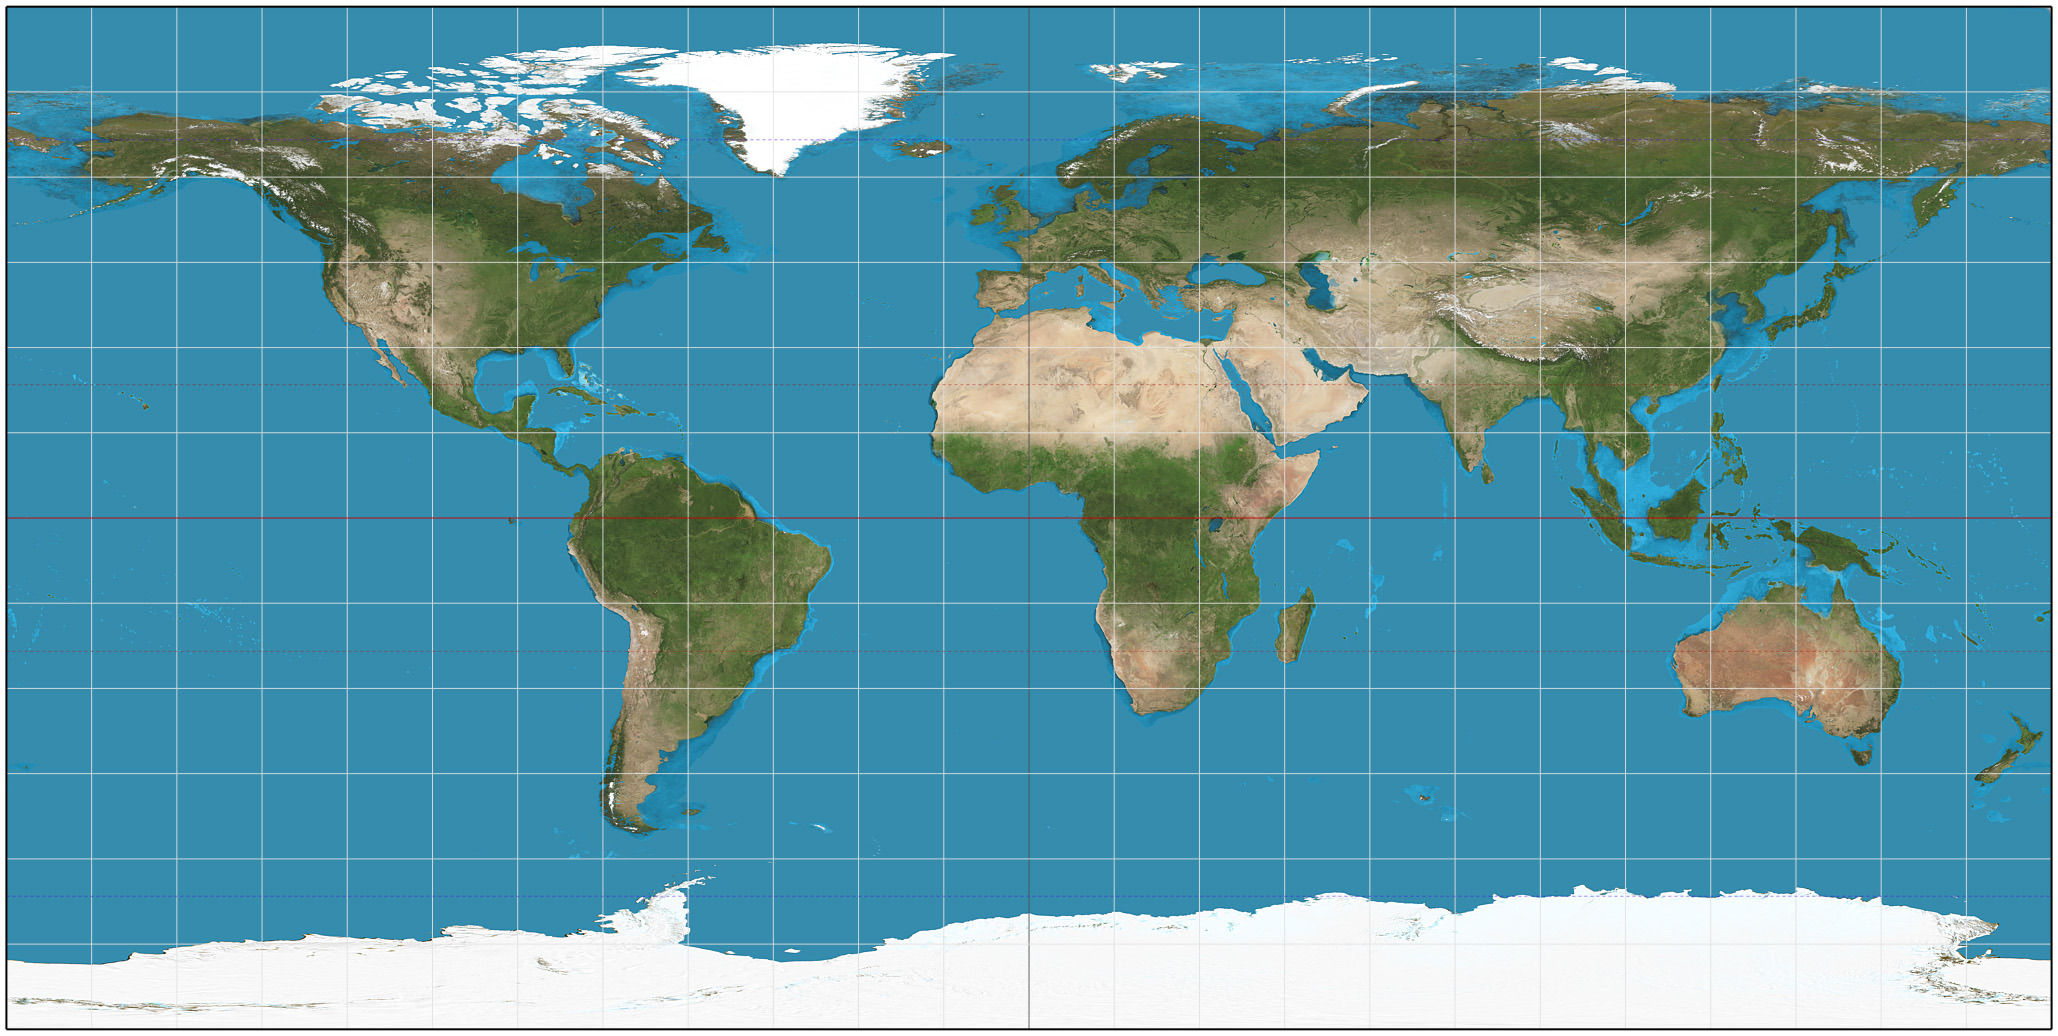
\includegraphics[width=.5\textwidth]{Images/Equirectangular_projection_SW.jpg}
    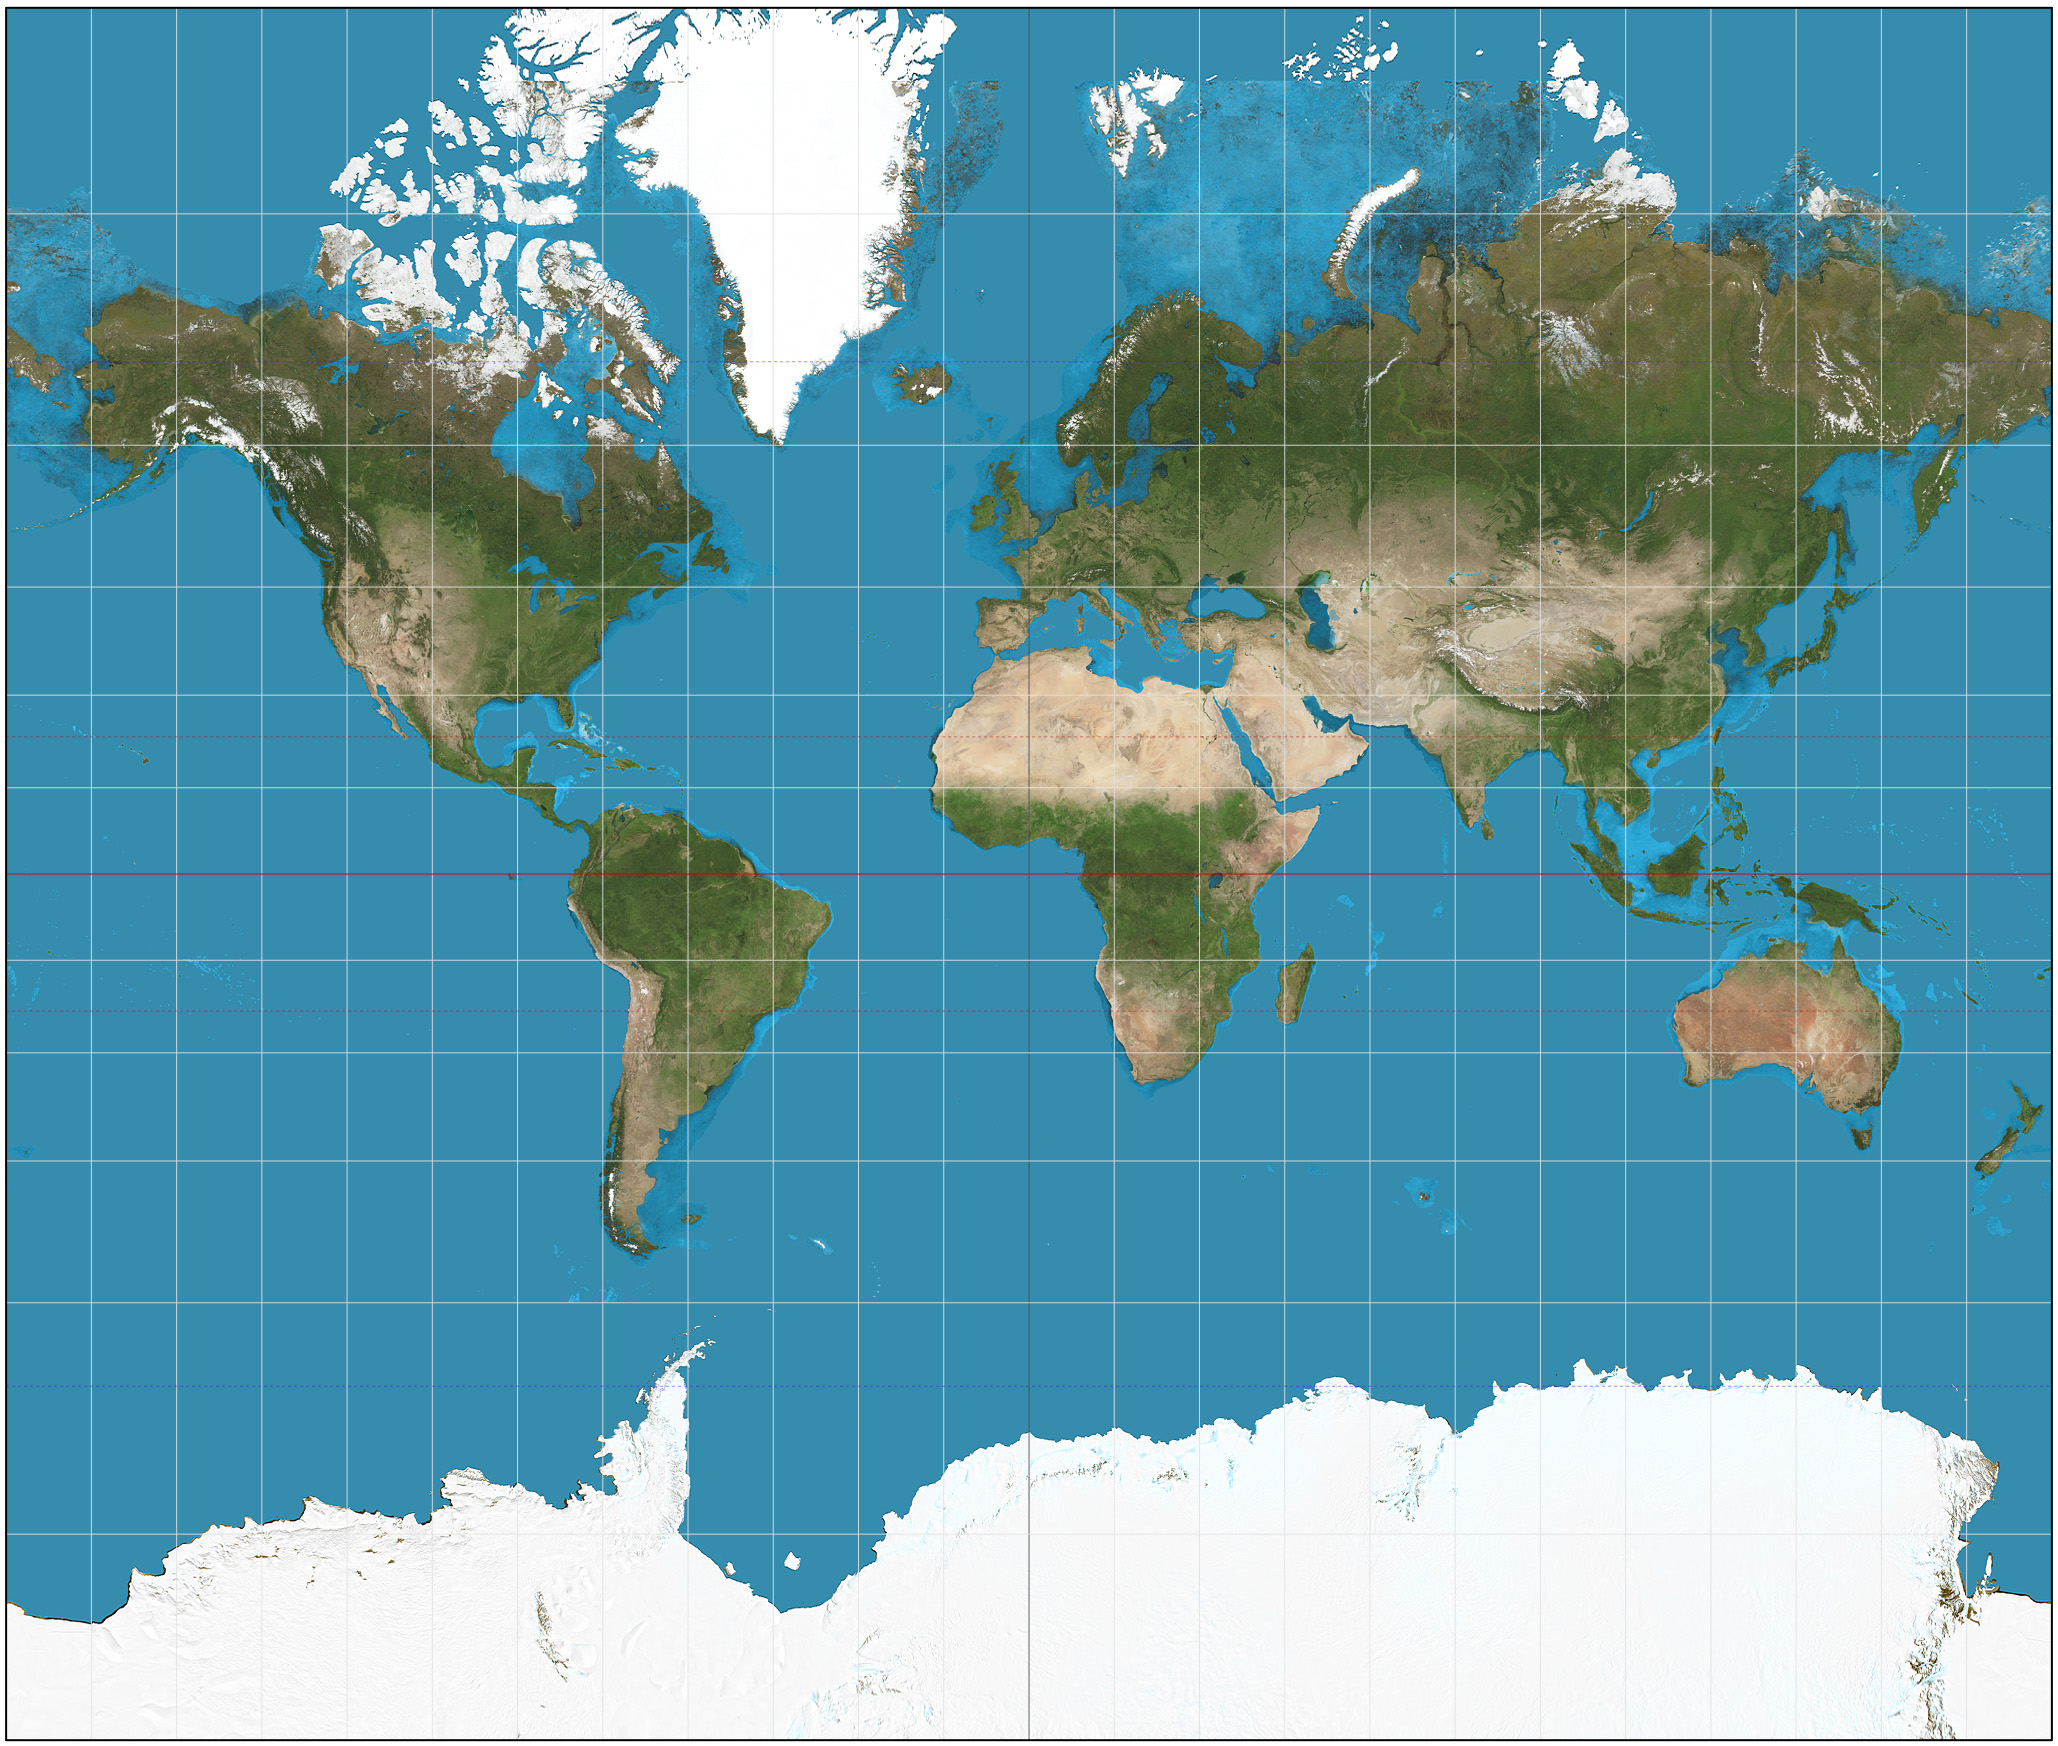
\includegraphics[width=.5\textwidth]{Images/Mercator_projection_SW.jpg}
    \quelle{\cite{img::mercator,img::equirectangular}}
    \caption[]{A map of the Earth mapped by the Equirectangular projection (left) and the Mercator projection (right). }
    \label{fig:projections}
  \end{minipage}
\end{figure}

In \Cref{fig:projections} we can see, what has already been described before.
In contrast to the Equirectangular projection on the left that looks visually compressed nearest the poles, the Mercator projection on the right stretches vertically in those parts.
This leads to a much more natural looking map, that would appeal more to the human perspective.

Nevertheless, the Equirectangular projection has a huge advantage, of allowing us to use the given coordinates without any additional calculations.
The Mercator projection requires one to apply a formula for each coordinate that is displayed.
Therefore, and due to the fact that the effect of the Mercator projection is quite low in most areas and particularly those that we will be displaying, the decision was made to use the Equirectangular projection for our visualization.

For the representation of nodes, circles are a common element and widely seen in graph visualizations.
However, as those visualizations are mostly used for smaller graphs (usually to explain the basic concepts of an algorithm) and we were going to display graphs with millions of nodes, we had to reconsider this representation of nodes.
As we know, at the end of every edge one node is to be found; we can clearly identify every node as long as the node is connected to any other node.
Therefore, we decided not to use any additional representation of nodes for the visualization, as they do not add any value and make the visualization more crowded.
We notice that we do not display nodes that are not connected to any other node.
As the only way for those nodes to play a role during the algorithm is beeing the start or the target node, the absence or presence of those nodes is not significant.

\paragraph{Edges.}

A common approach for dipplaying edges is to represent them by straight lines.
The length of the edges is generally reflected by the length of the lines in most cases.
However, we need to respect that it is possible, that the linear distance of two nodes, which is displayed by the linear representation, can diverge quite a lot from the real length of the edge in some cases.
In addition, as we use the Equirectangular projection, the lines are distorted horizontally depending on their proximity to the poles.

In order to also represent the speed of an edge, we can color the edge according to its speed.
By using the HSV color space we achieved a seamless color transition from red for 0 km/h, yellow for a speed of approximately 60 km/h and green for the fastest edges with a speed of 120 km/h and more.
Using HSV we are be able to outline edges with a speed of 240 km/h without any issues in comprehensibility.


\paragraph{Tiles.}
One way of visualizing the tiles, that does not require any new element, is display all edges of the tile in a lighter color as soon as the tile is accessed the first time.
This representation has the disadvantage that we can only possible to distinguish tiles along the outer graph.

By using rectangles to outline the tiles it is possible to differentiate tiles in every region of the graph.
Due to the Equirectangular projection, all those rectangles have the same size and are (as in the previous method) displayed on their first access.


\section{Displaying the Algorithm} \label{algorithm}

In this section, we describe how we used the elements, introduced in \Cref{graph}, for displaying how the graph evolves during the ongoing algorithm.

\subsection{Basics} \label{basic}

\paragraph{Combining the Elements.}

For a basic edge-based visualization we commence with an empty space and then add one edge after another as they are processed by the algorithm.
This will happen either automatically or on request by pressing a key.

For now, we assume displaying the correct region of the graph is not a problem.

\begin{figure}
    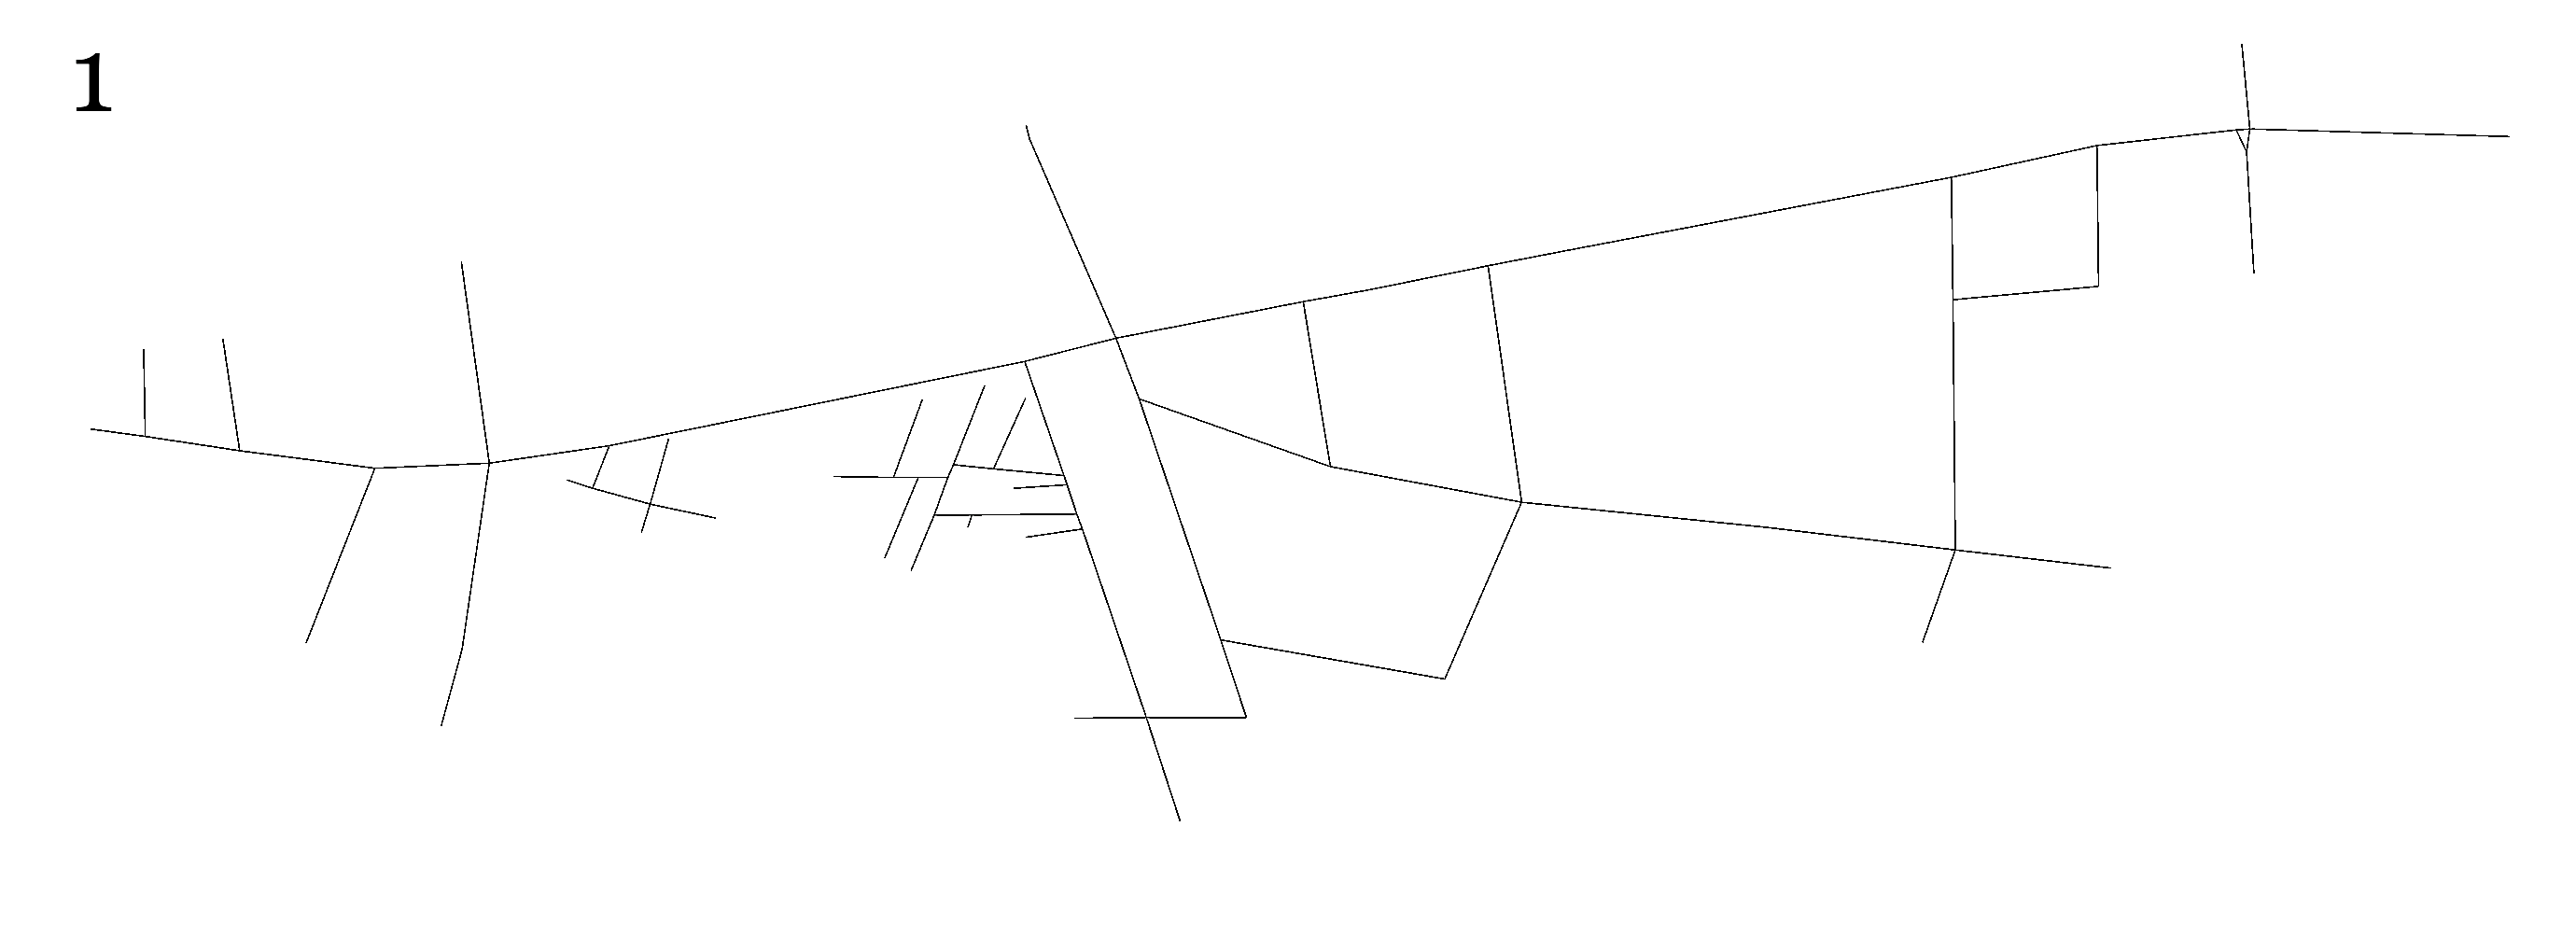
\includegraphics[width=.5\textwidth]{Images/vis-step-one.png}
    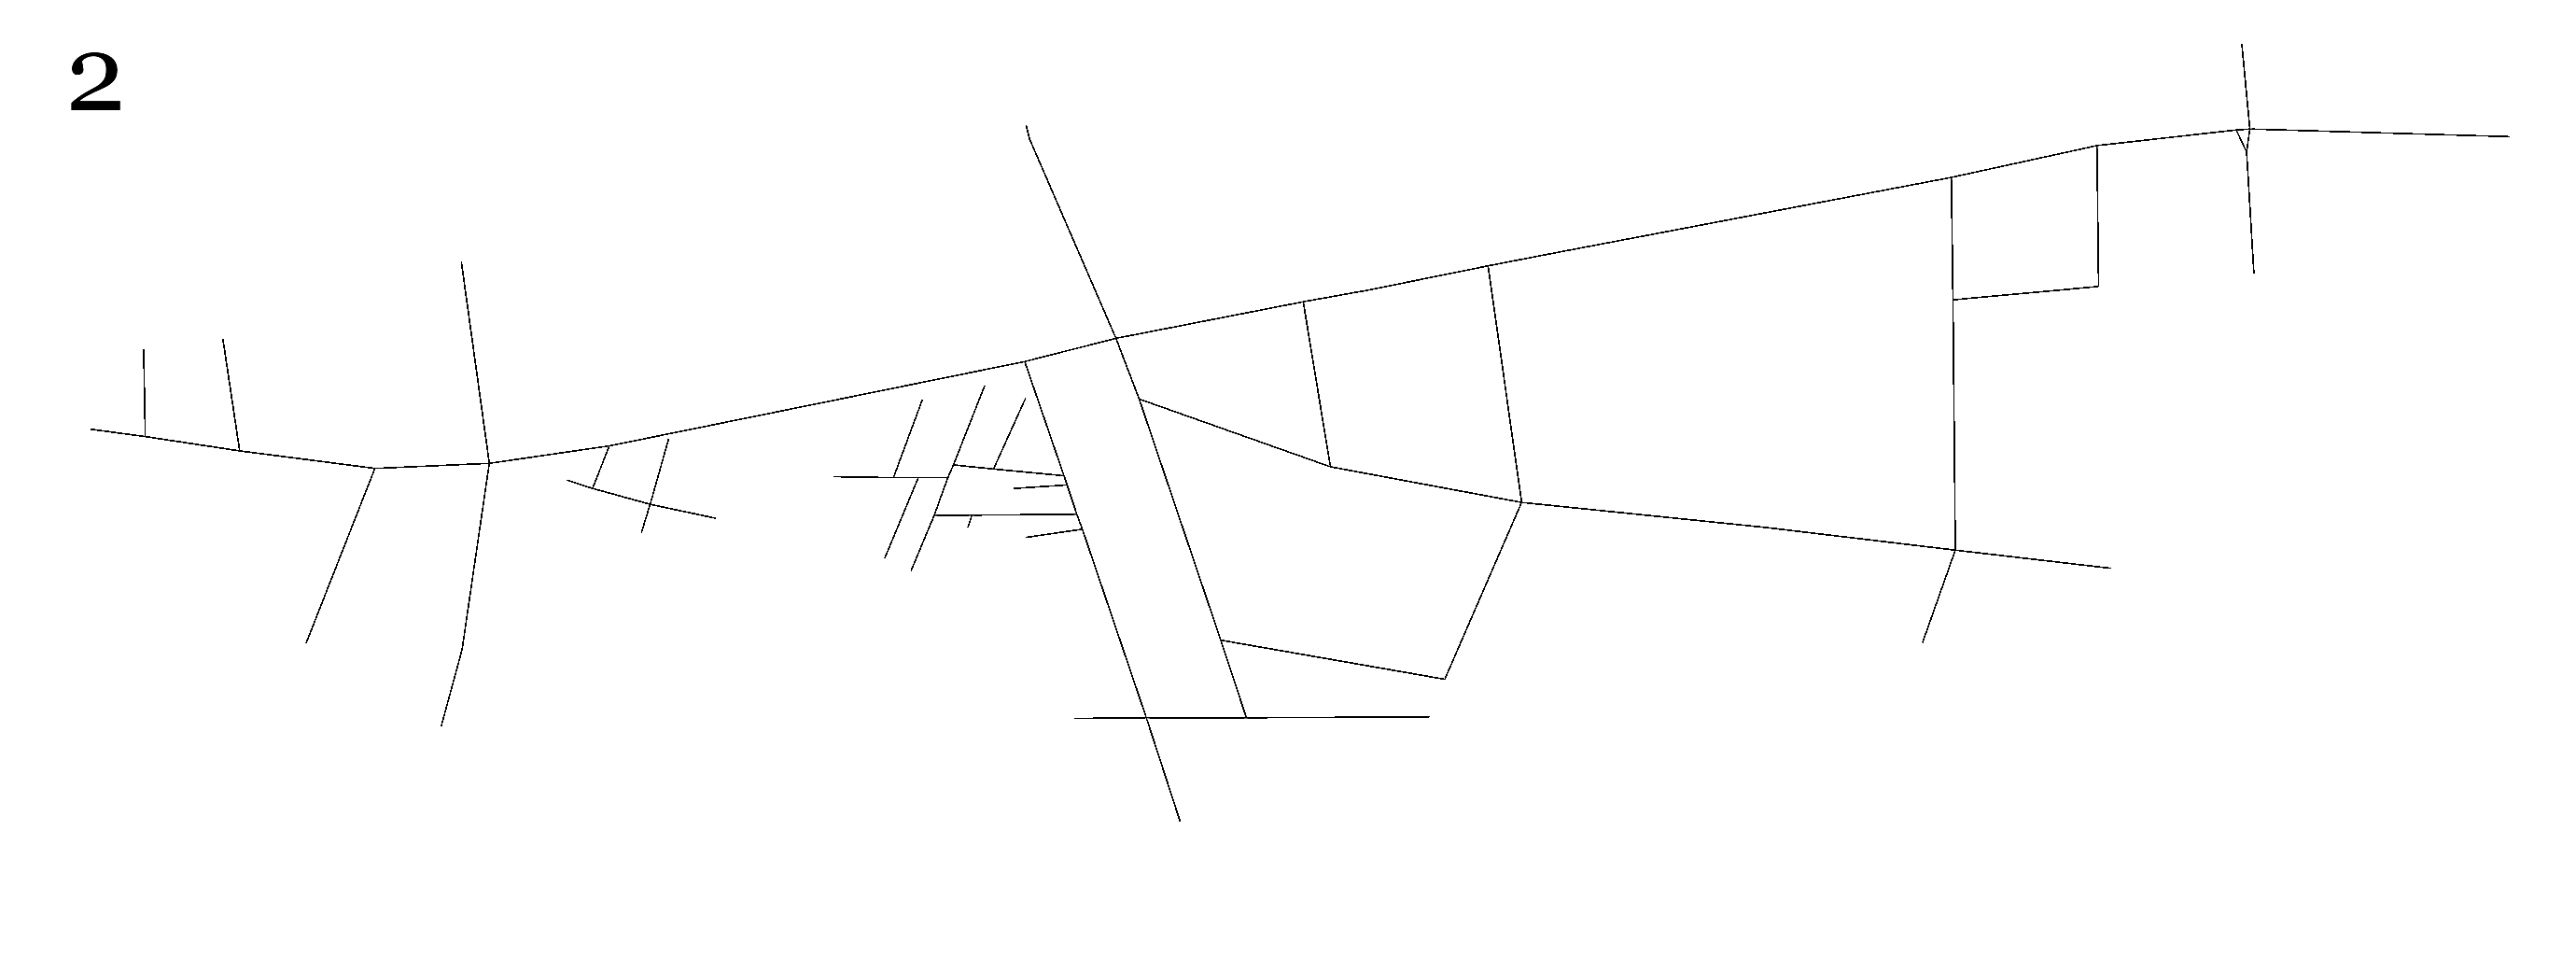
\includegraphics[width=.5\textwidth]{Images/vis-step-two.png}
\caption{Two consecutive steps in the visualization. Every black line represents an edge.}
\label{fig:two-steps}
\end{figure}
\todo{mehr graph}

In \Cref{fig:two-steps} we can see that we achieved a good basic understanding of how the algorithm evolves.
The tiles can be visualized in a similar way.
A tile is always displayed whenever its first edge is processed.

\begin{figure}
    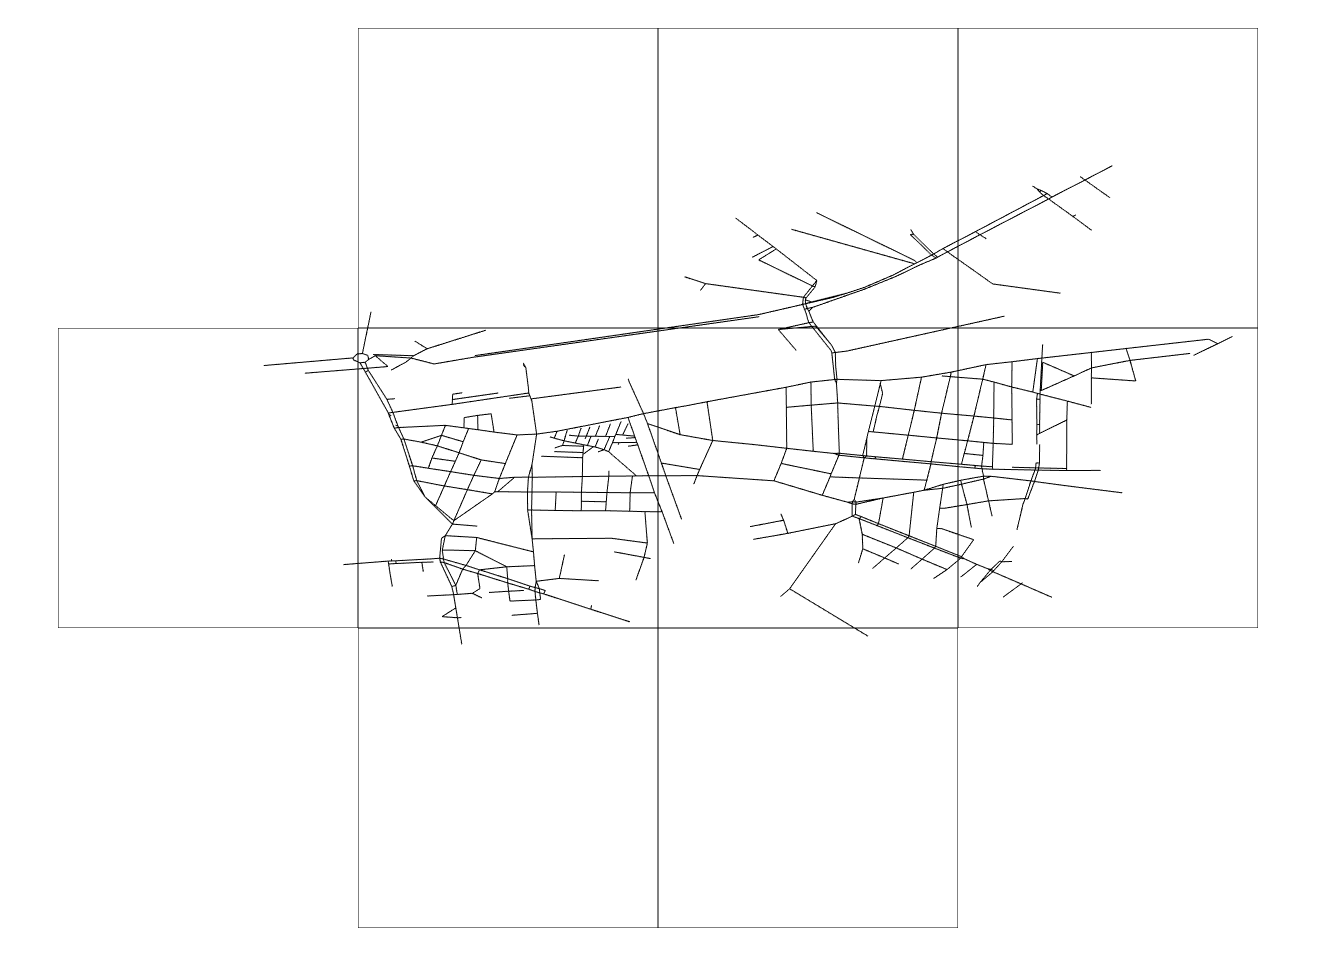
\includegraphics[width=\textwidth]{Images/vis-rectangular-tiles-small.png}
\caption[]{Extension of \Cref{fig:two-steps}. In addition tiles are represented by rectangles.}
\label{fig:rectangle_tiles}
\end{figure}

The strategy of displaying edges and tiles as seen in  \Cref{fig:rectangle_tiles} works great on smaller routes and it is possible to track the state of the algorithm quite well.

\begin{figure}
    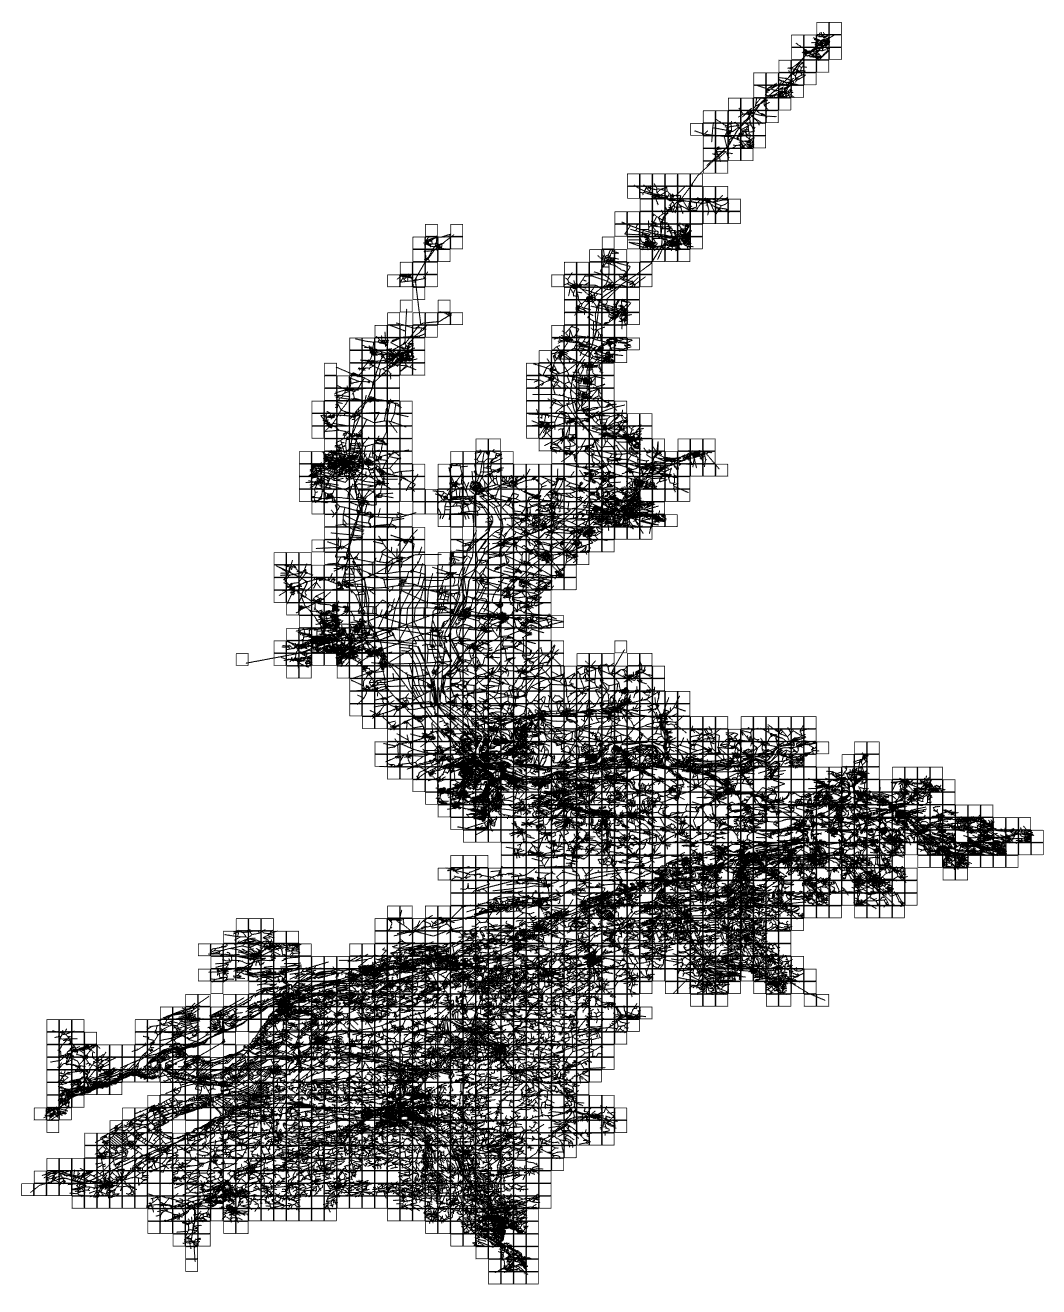
\includegraphics[width=\textwidth]{Images/vis-rectangular-tiles.png}
\caption[]{Using the same method as in \Cref{fig:rectangle_tiles}, but on a bigger route.}
\label{fig:rectangle_tiles_big}
\end{figure}

On bigger routes, however, this visualization lacks in comprehensibility as we can see in \Cref{fig:rectangle_tiles_big}.
In addition, we experienced performance issues due to the amount of displayed elements and one step is hard to distinguish from its predecessor.
Thus, for long distance queries, it makes sense to remove the edges from the visualization.

\begin{figure}
        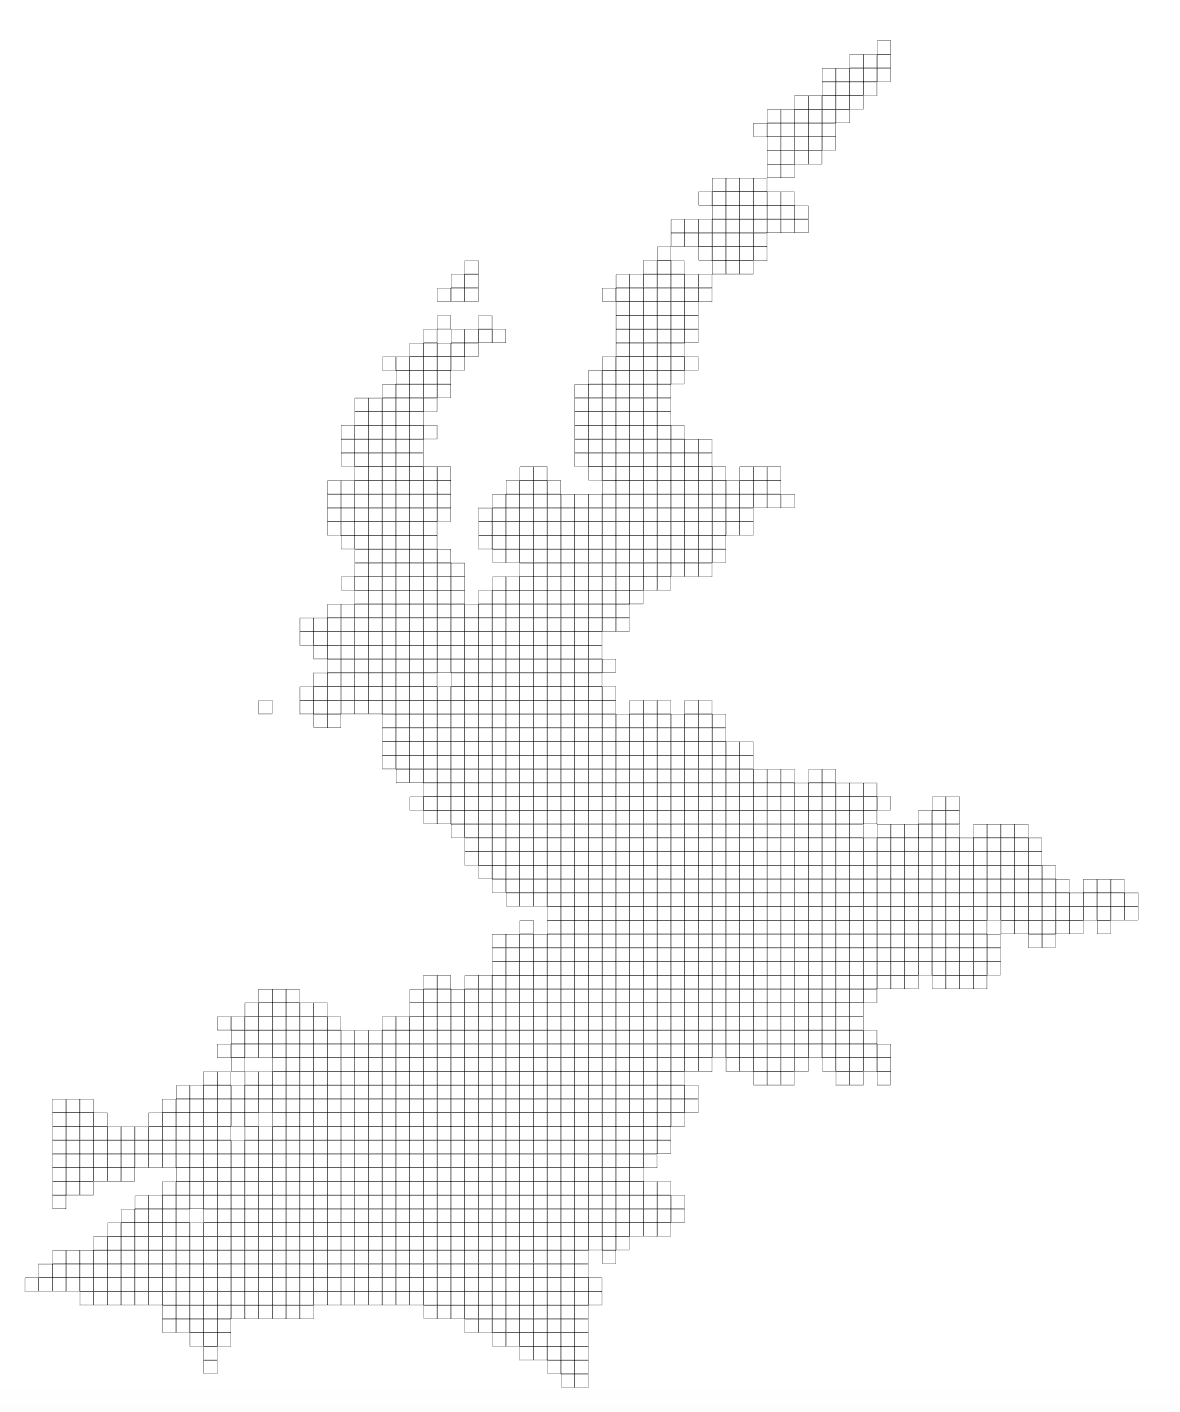
\includegraphics[width=\textwidth]{Images/vis-only-rectangles.png}
\caption[]{Representing tiles only through rectangles.}
\label{fig:only_rectangles}
\end{figure}

In \Cref{fig:only_rectangles} we see an uncluttered representation based on tiles.
By removing the edges we also experienced a tremendous performance boost.


\paragraph{Outlining the Current Step.}

In the tile-based visualization, from \Cref{fig:only_rectangles}, it is difficult to detact when a tile is added to the graph.
Furthermore, it is impossible to notice which tile the algorithm is currently processing.
Therefore, a trivial approach is to color the tile in which the algorithm is currently processing edges.

For increasing the level of understanding as to which route the algorithm will seek to find and also find out how far the algorithm already proceeded to find this path, we added the resulting path of the algorithm to the visualization.
This is, of course, only possible in post-execution visualizations.

\begin{figure}
        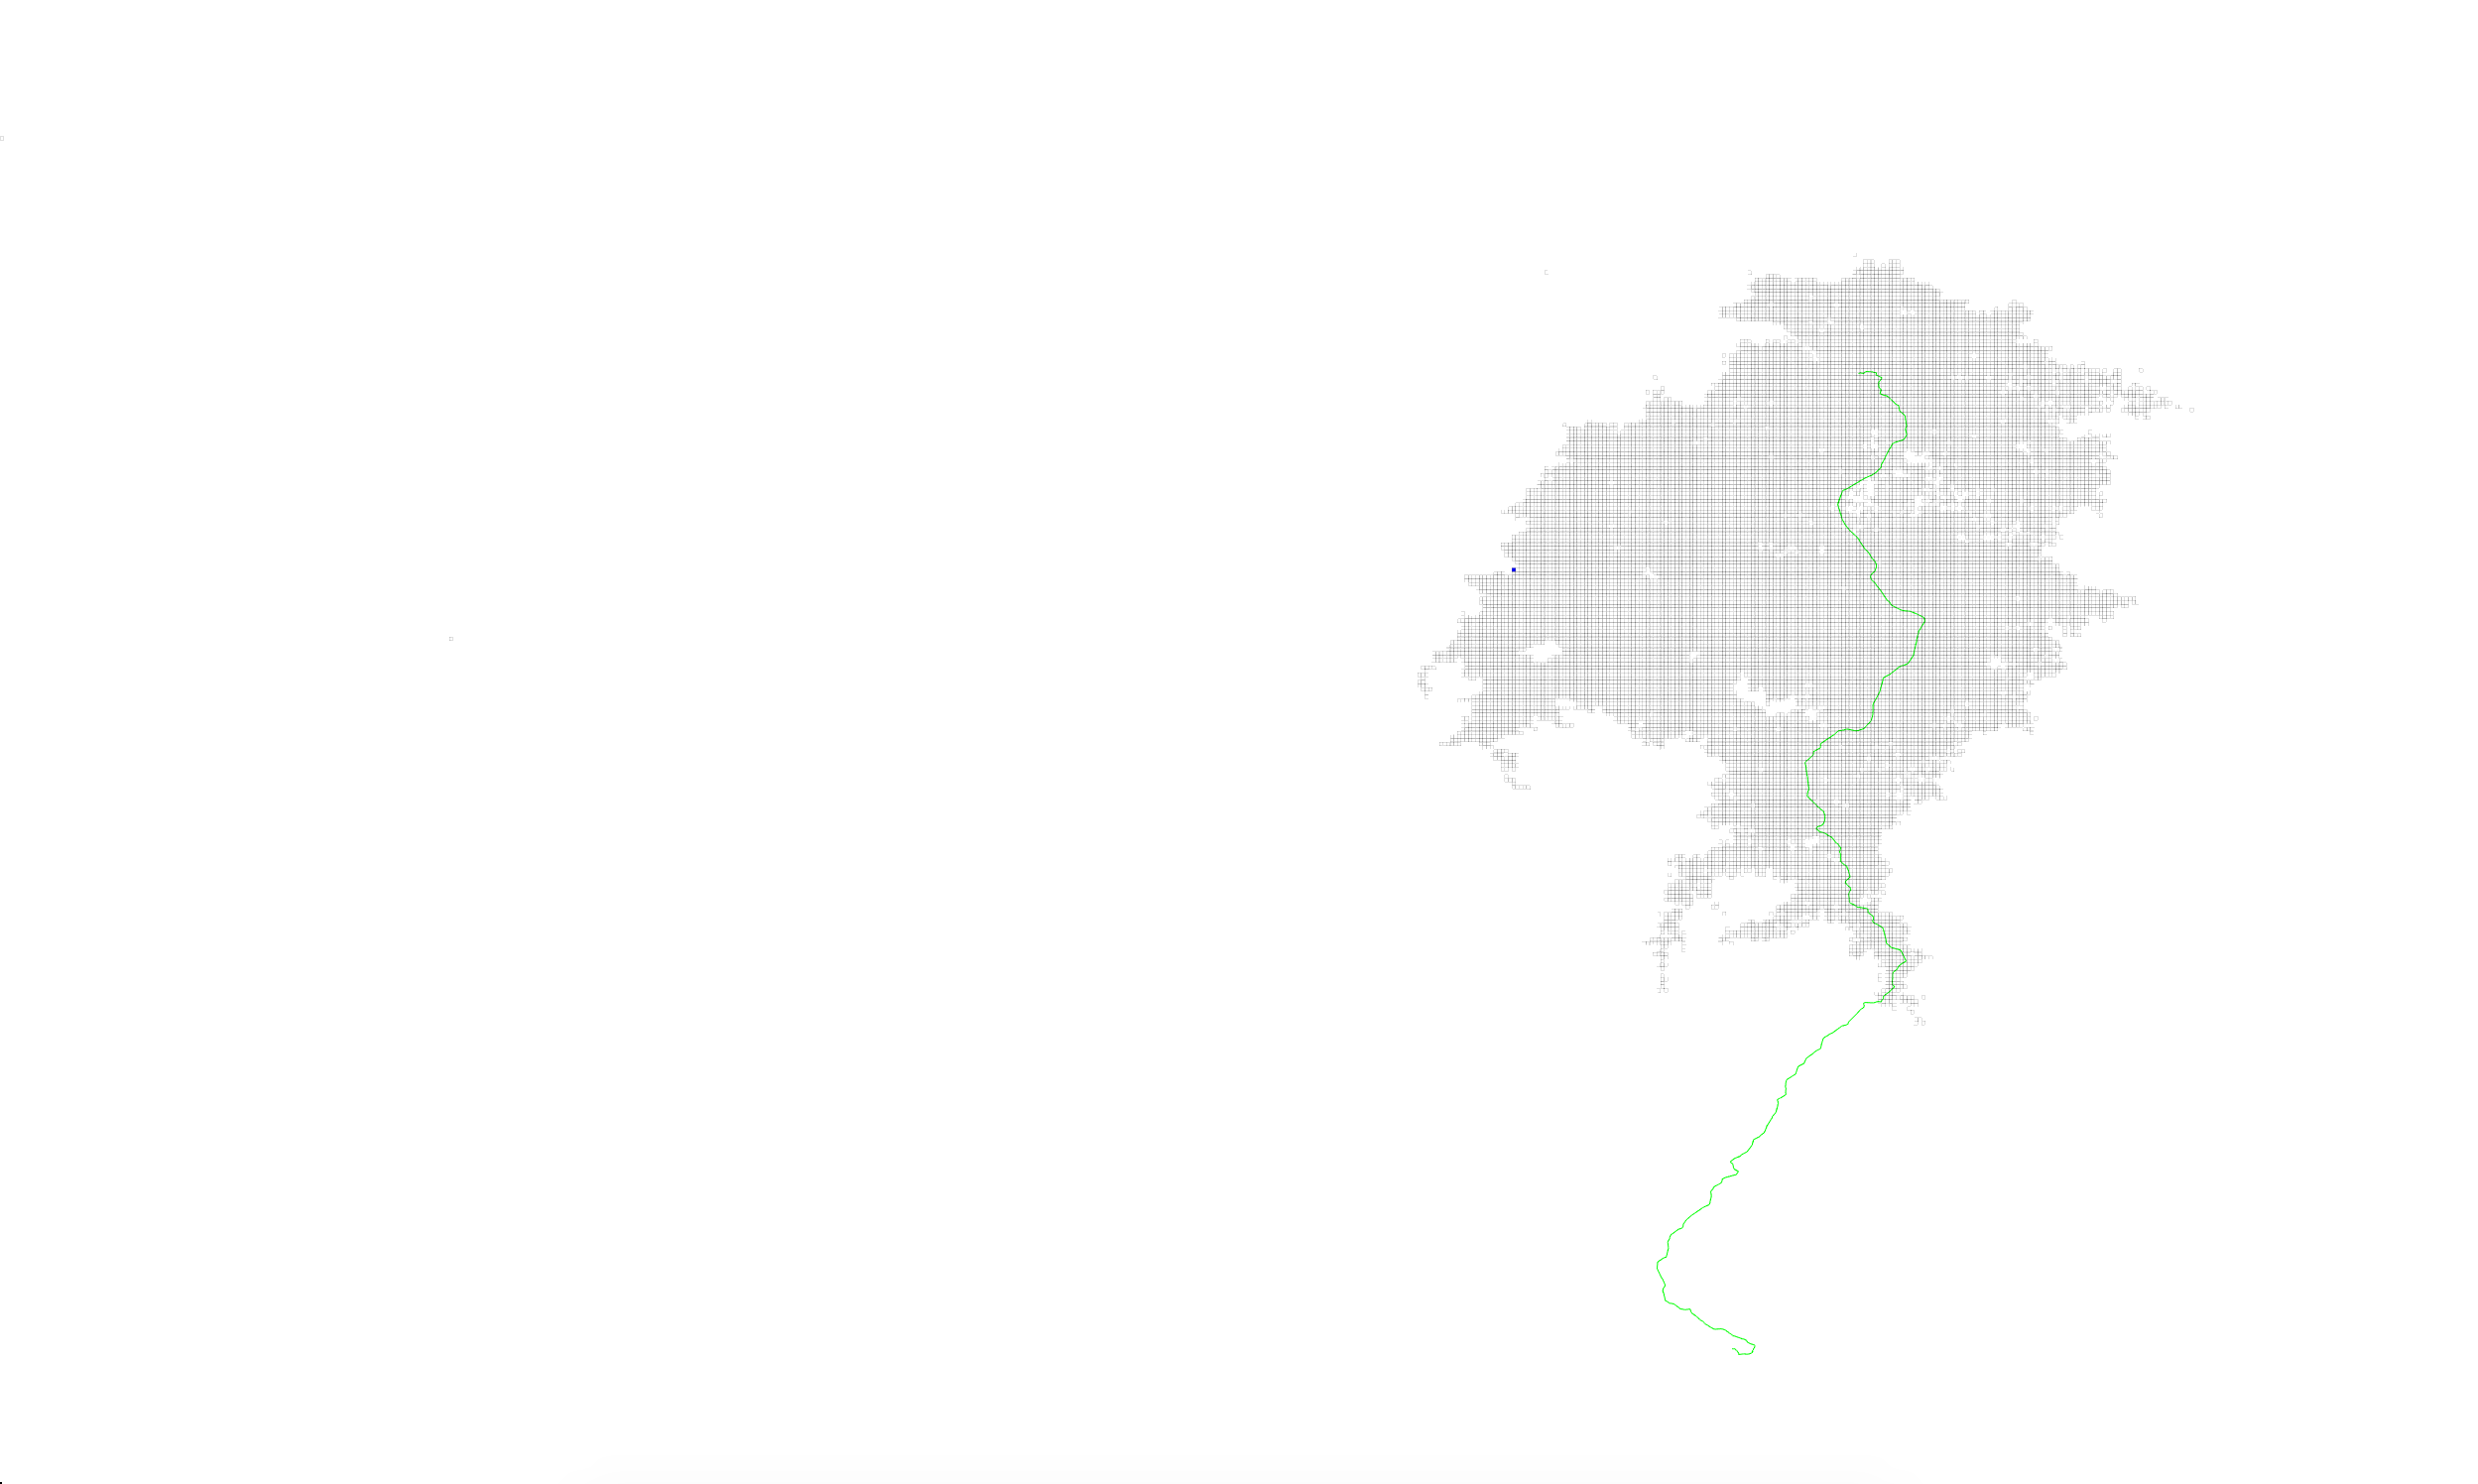
\includegraphics[width=\textwidth]{Images/vis-current-tile.png}
\caption[]{Coloring the tile that is processed blue. The searched path is represented in green.}
\label{fig:color_current_tile}
\end{figure}

Even though this method enables us to see which tile is processed in a single image, the information gained in this feature is quite small, as we can see in \Cref{fig:color_current_tile}.
For learning something about the algorithm, knowing what tile is loaded in one specific step is not enough.
Rather, knowledge about many successive steps is necessary.
This could be achieved by just running the visualization, but when doing this the colored tile is barely visible.
Thus we had to search and discover a more compatible method of showing what is going on.

We came up with a method we called tile-aging.
The method evolved from the previously mentioned method; it serves as a continuation, but instead of phasing-out the tile color rapidly, it phases-out tile color over time.
Therefore, the tile becomes slightly brighter at every step of the algorithm.

\begin{figure}
    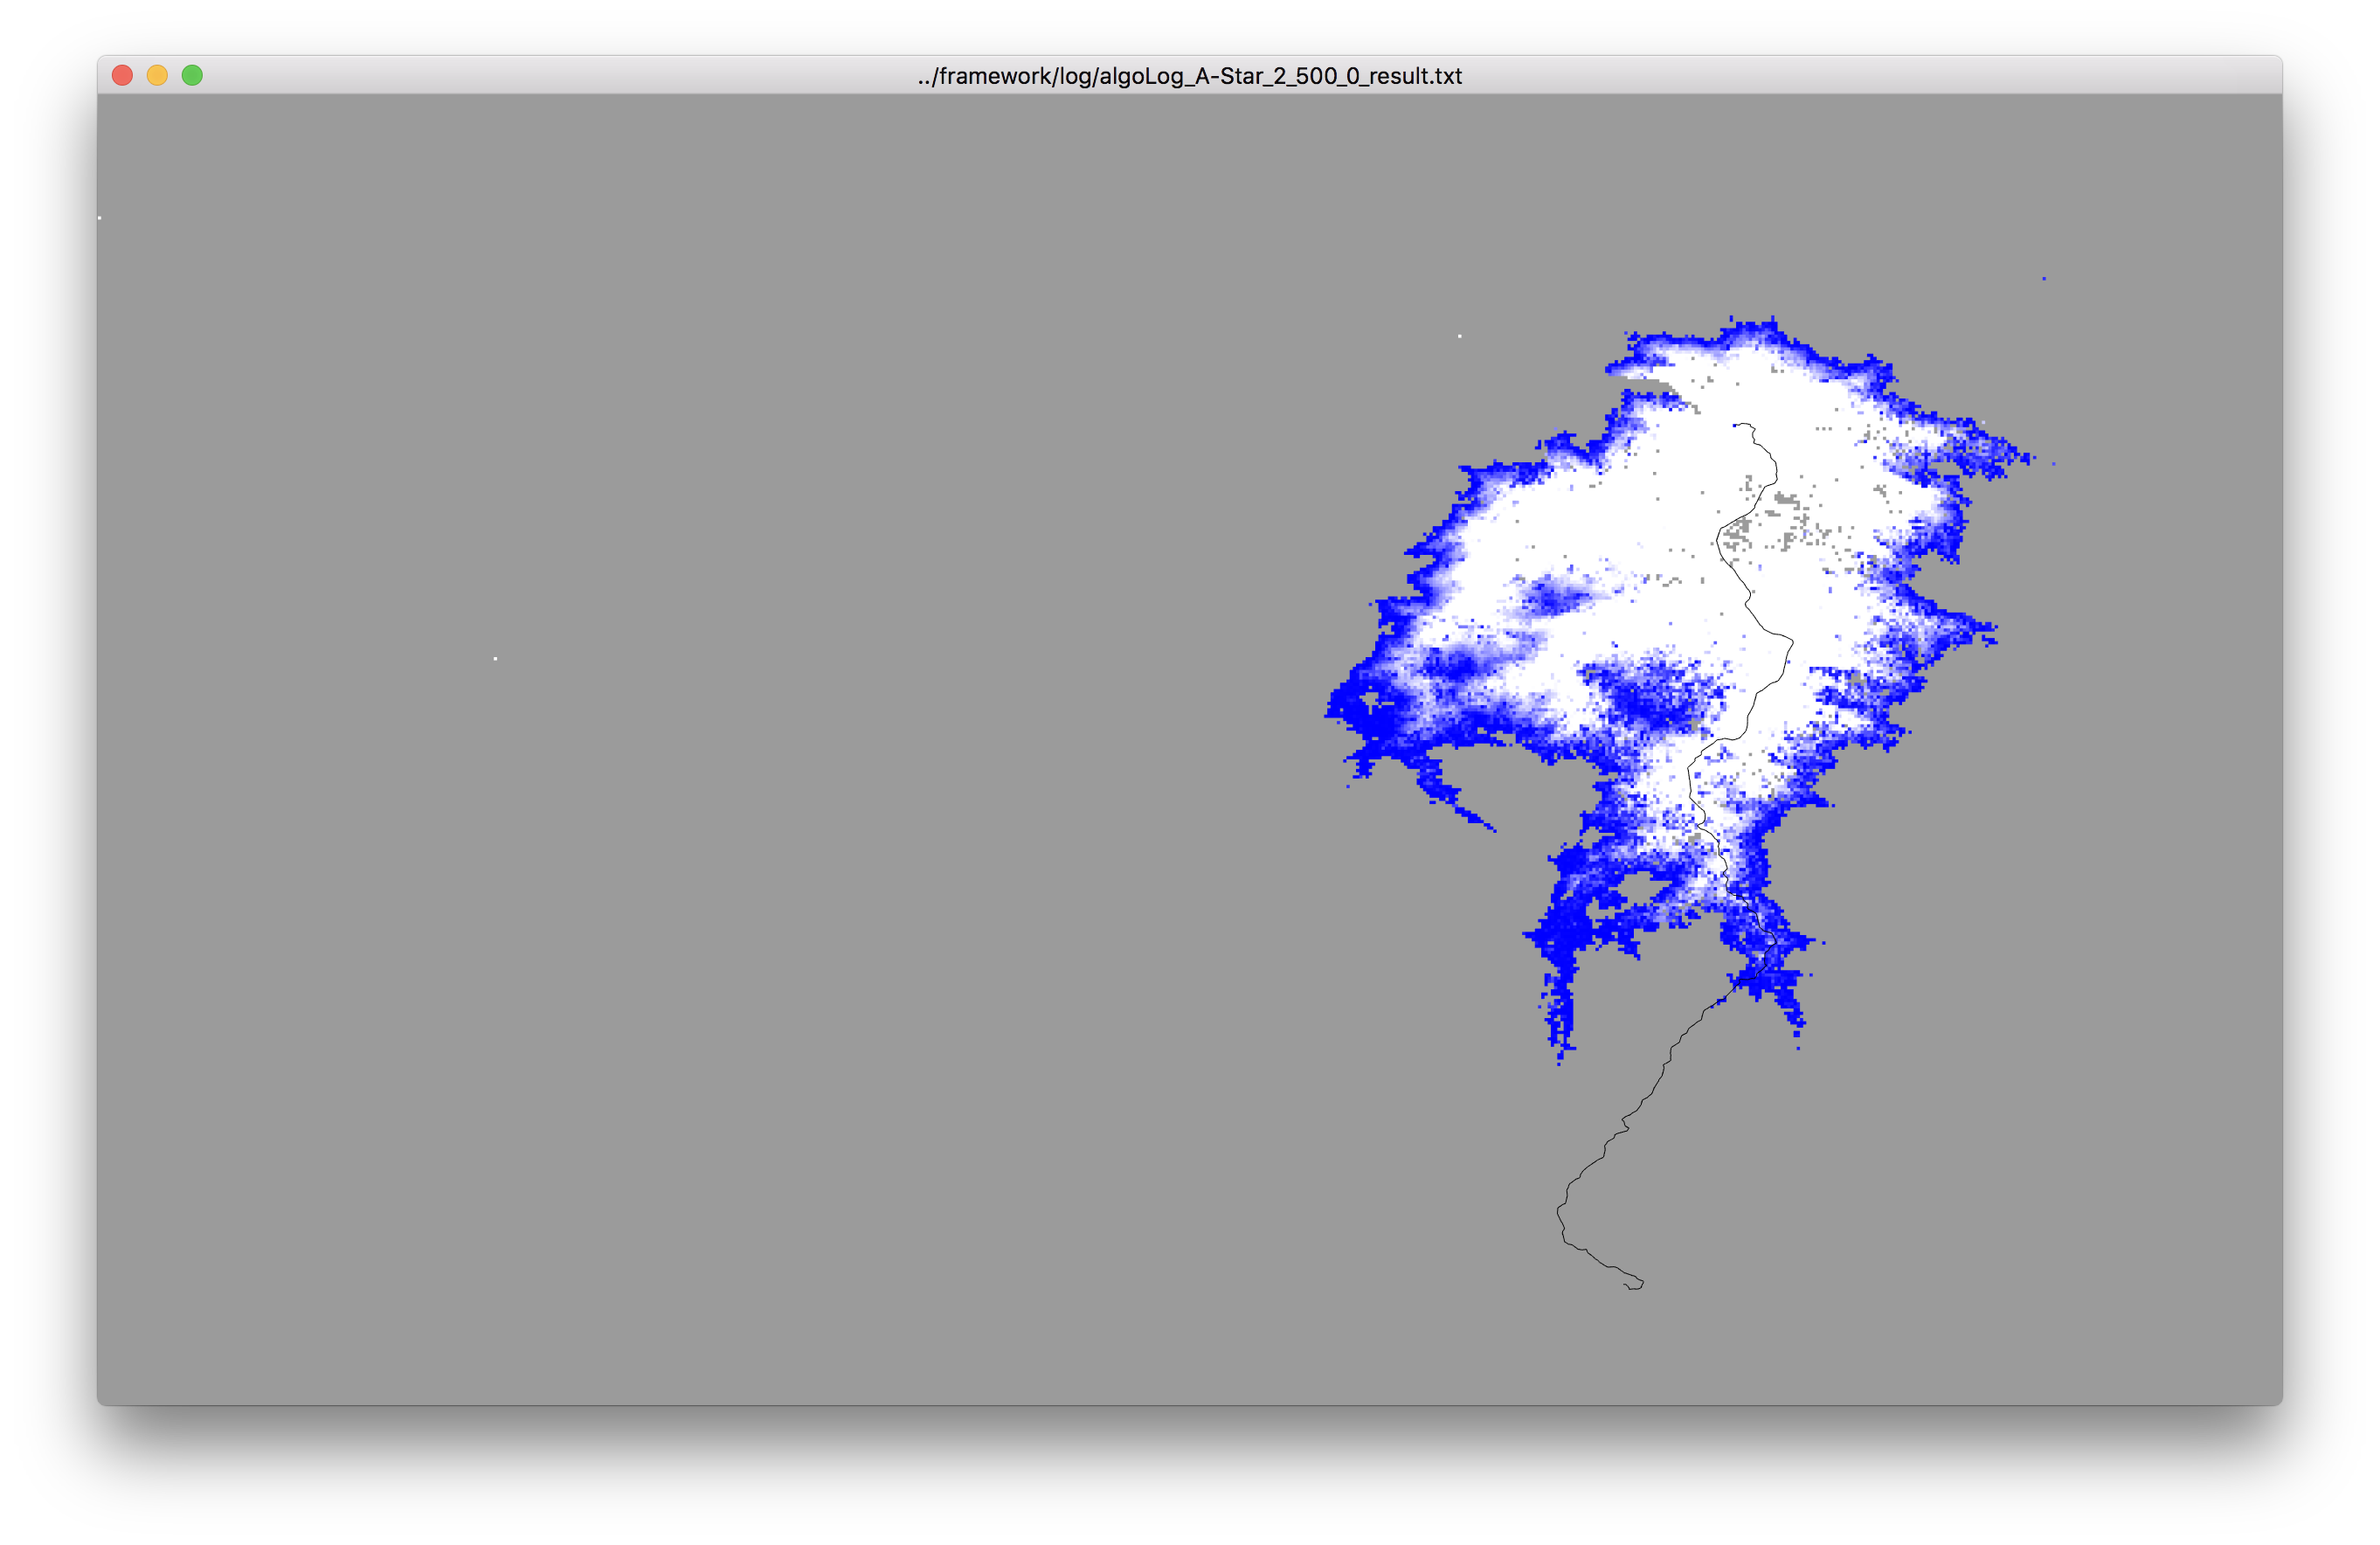
\includegraphics[width=\textwidth]{Images/vis-aged-coloring.png}
\caption[]{Tile-aging. Newly loaded tiles are colored blue and get brighter the longer they have not been loaded. The searched path is represented in green.}
\label{fig:color_aged_tile}
\end{figure}

In \Cref{fig:color_aged_tile} we see that this approach leads to a much better understanding of the sequence of tile-loads.
Therefore, it improves comprehensibility us to how the algorithm performs on the underlying graph.

In the example displayed in \Cref{fig:color_aged_tile}, we notice that most of the recently loaded tiles are located on the outside of the explored graph, but there are three larger areas in the inner graph as well.
After an examination of those areas we found a simple explanation.
The larger recently processed areas are located in-between highways.
Therefore the algorithm observes the highways first and then slowly spreads outwards from the highway exits.

\paragraph{Showing the Correct Region of the Graph.}
In this paragraph, we are going to explain something we previously took for granted.
In one way or another, we have to decide where we want to place the elements in the visualization.
We seek to show the same element at exactly the same spot in the entire visualization.
Therefore, the visualization needs to consider which region of the graph it seeks to show before it displays the first element.
As the displayed graph grows as the algorithm progresses there is the risk of growing out of the screen when we estimate the final graph too small.
On the other side, a graph that is estimated to big, which would result in much unused space on out screen.

% As the displayed graph expands and the algorithm progresses, graph size problems might occur.
% The graph might be smaller or larger than the desired screen area.
% Unused space is to be avoided, therefore a smaller graph must fit into a larger frame.
%
% This risk
%  is the risk of growing out of the screen when we estimating the final graph as too small.
% On the other side, a graph that is estimated to big, which would result in much unused space on out screen.

We considered multiple approaches to solve this issue.
Firstly, we developed an estimation method that estimates the extent of the explored graph of the fully evolved algorithm.
For estimation purposes, this method uses the linear distance between start and target node as the basis.
Because we need to make sure that the visualization shows everything that is going to happen during the algorithm, it uses a little more than the amount of distance between start and target node; this length is used as the radius of a circle around the start node.
The dimensions of this circle then fit into the visualization borders, as we assume that the final graph will fill this circle.

\begin{figure}
    \fbox{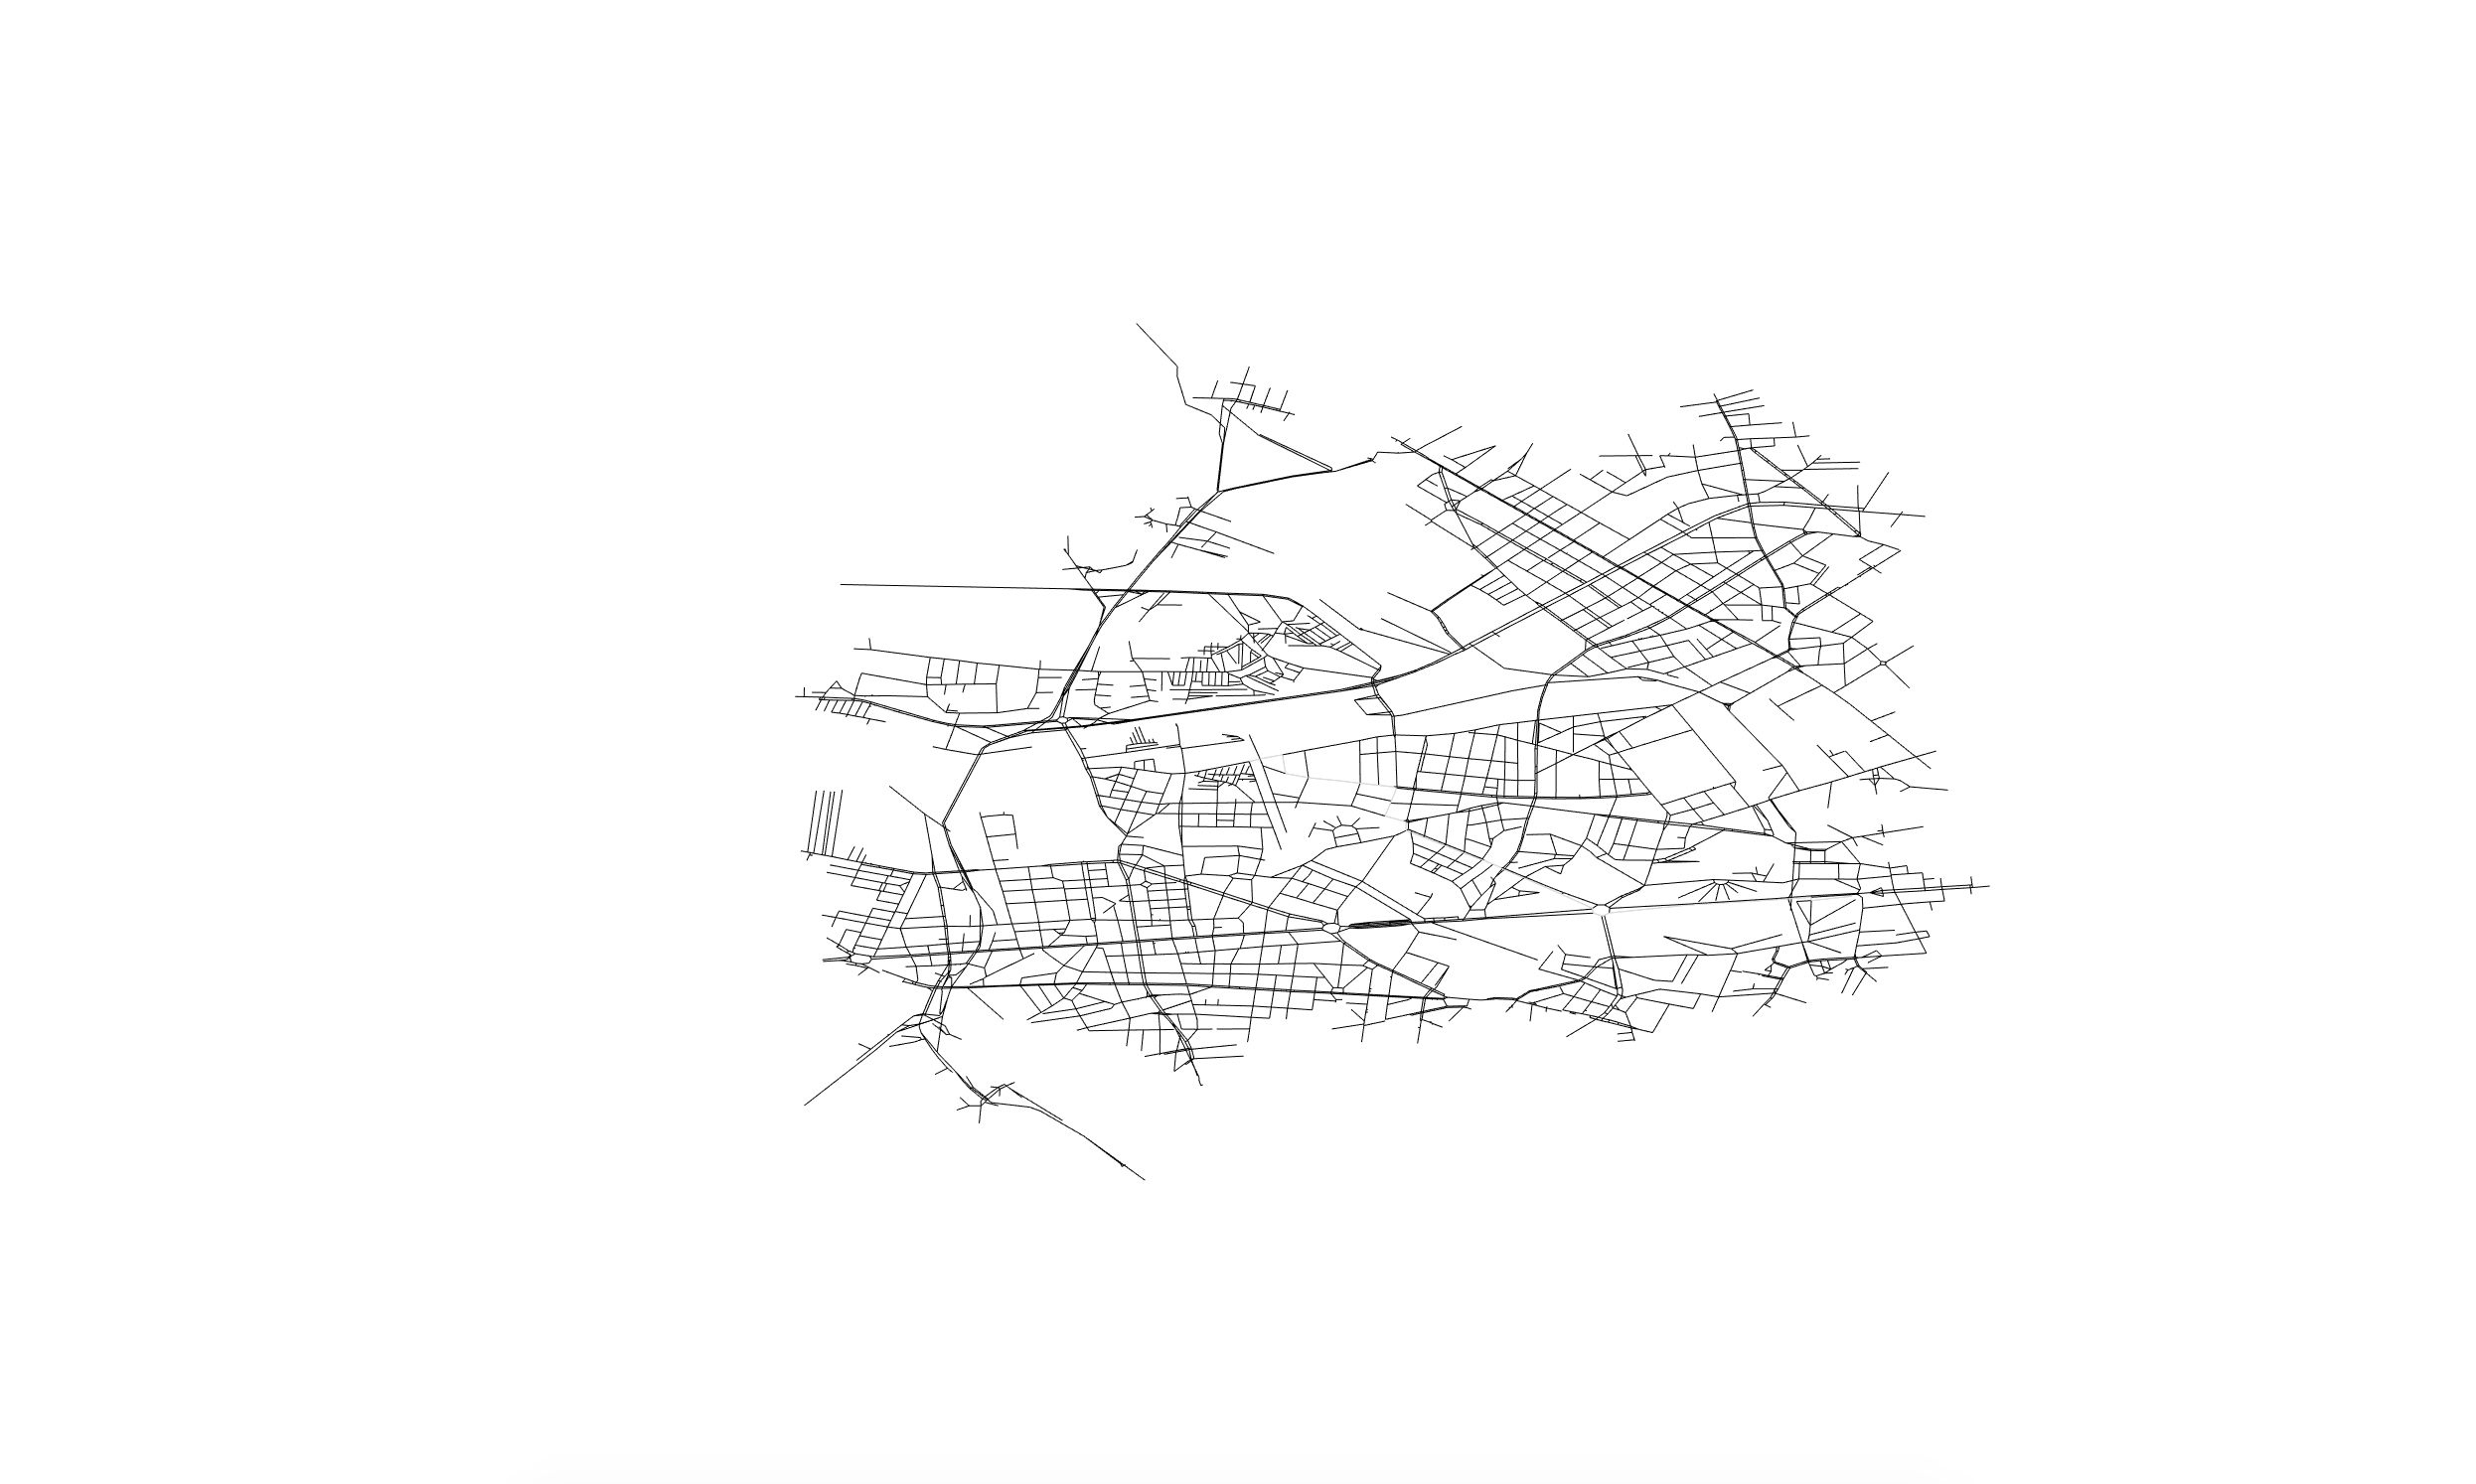
\includegraphics[width=\textwidth]{Images/vis-estimation.png}}
\caption[]{Final state of the visualization, using the Estimation method on the edge-based visualization.}
\label{fig:estimation}
\end{figure}

In \Cref{fig:estimation} we can see that we notice a significant amount of unused space, with this estimation.
Although this estimation is quite generous, the actual graph might trespass the estimated circle.
In general, it is, of course, possible to provide a better estimation, but the more precise the estimation, the more information we need concerning the specific algorithm and its underlying graph, which we must avoid.

Another method is to iterate over the algorithm before visualizing it, and therefore find the exact borders of the graph.
With this knowledge, we could then adjust the shown section to exactly fit the fully evolved graph.

\begin{figure}
    \fbox{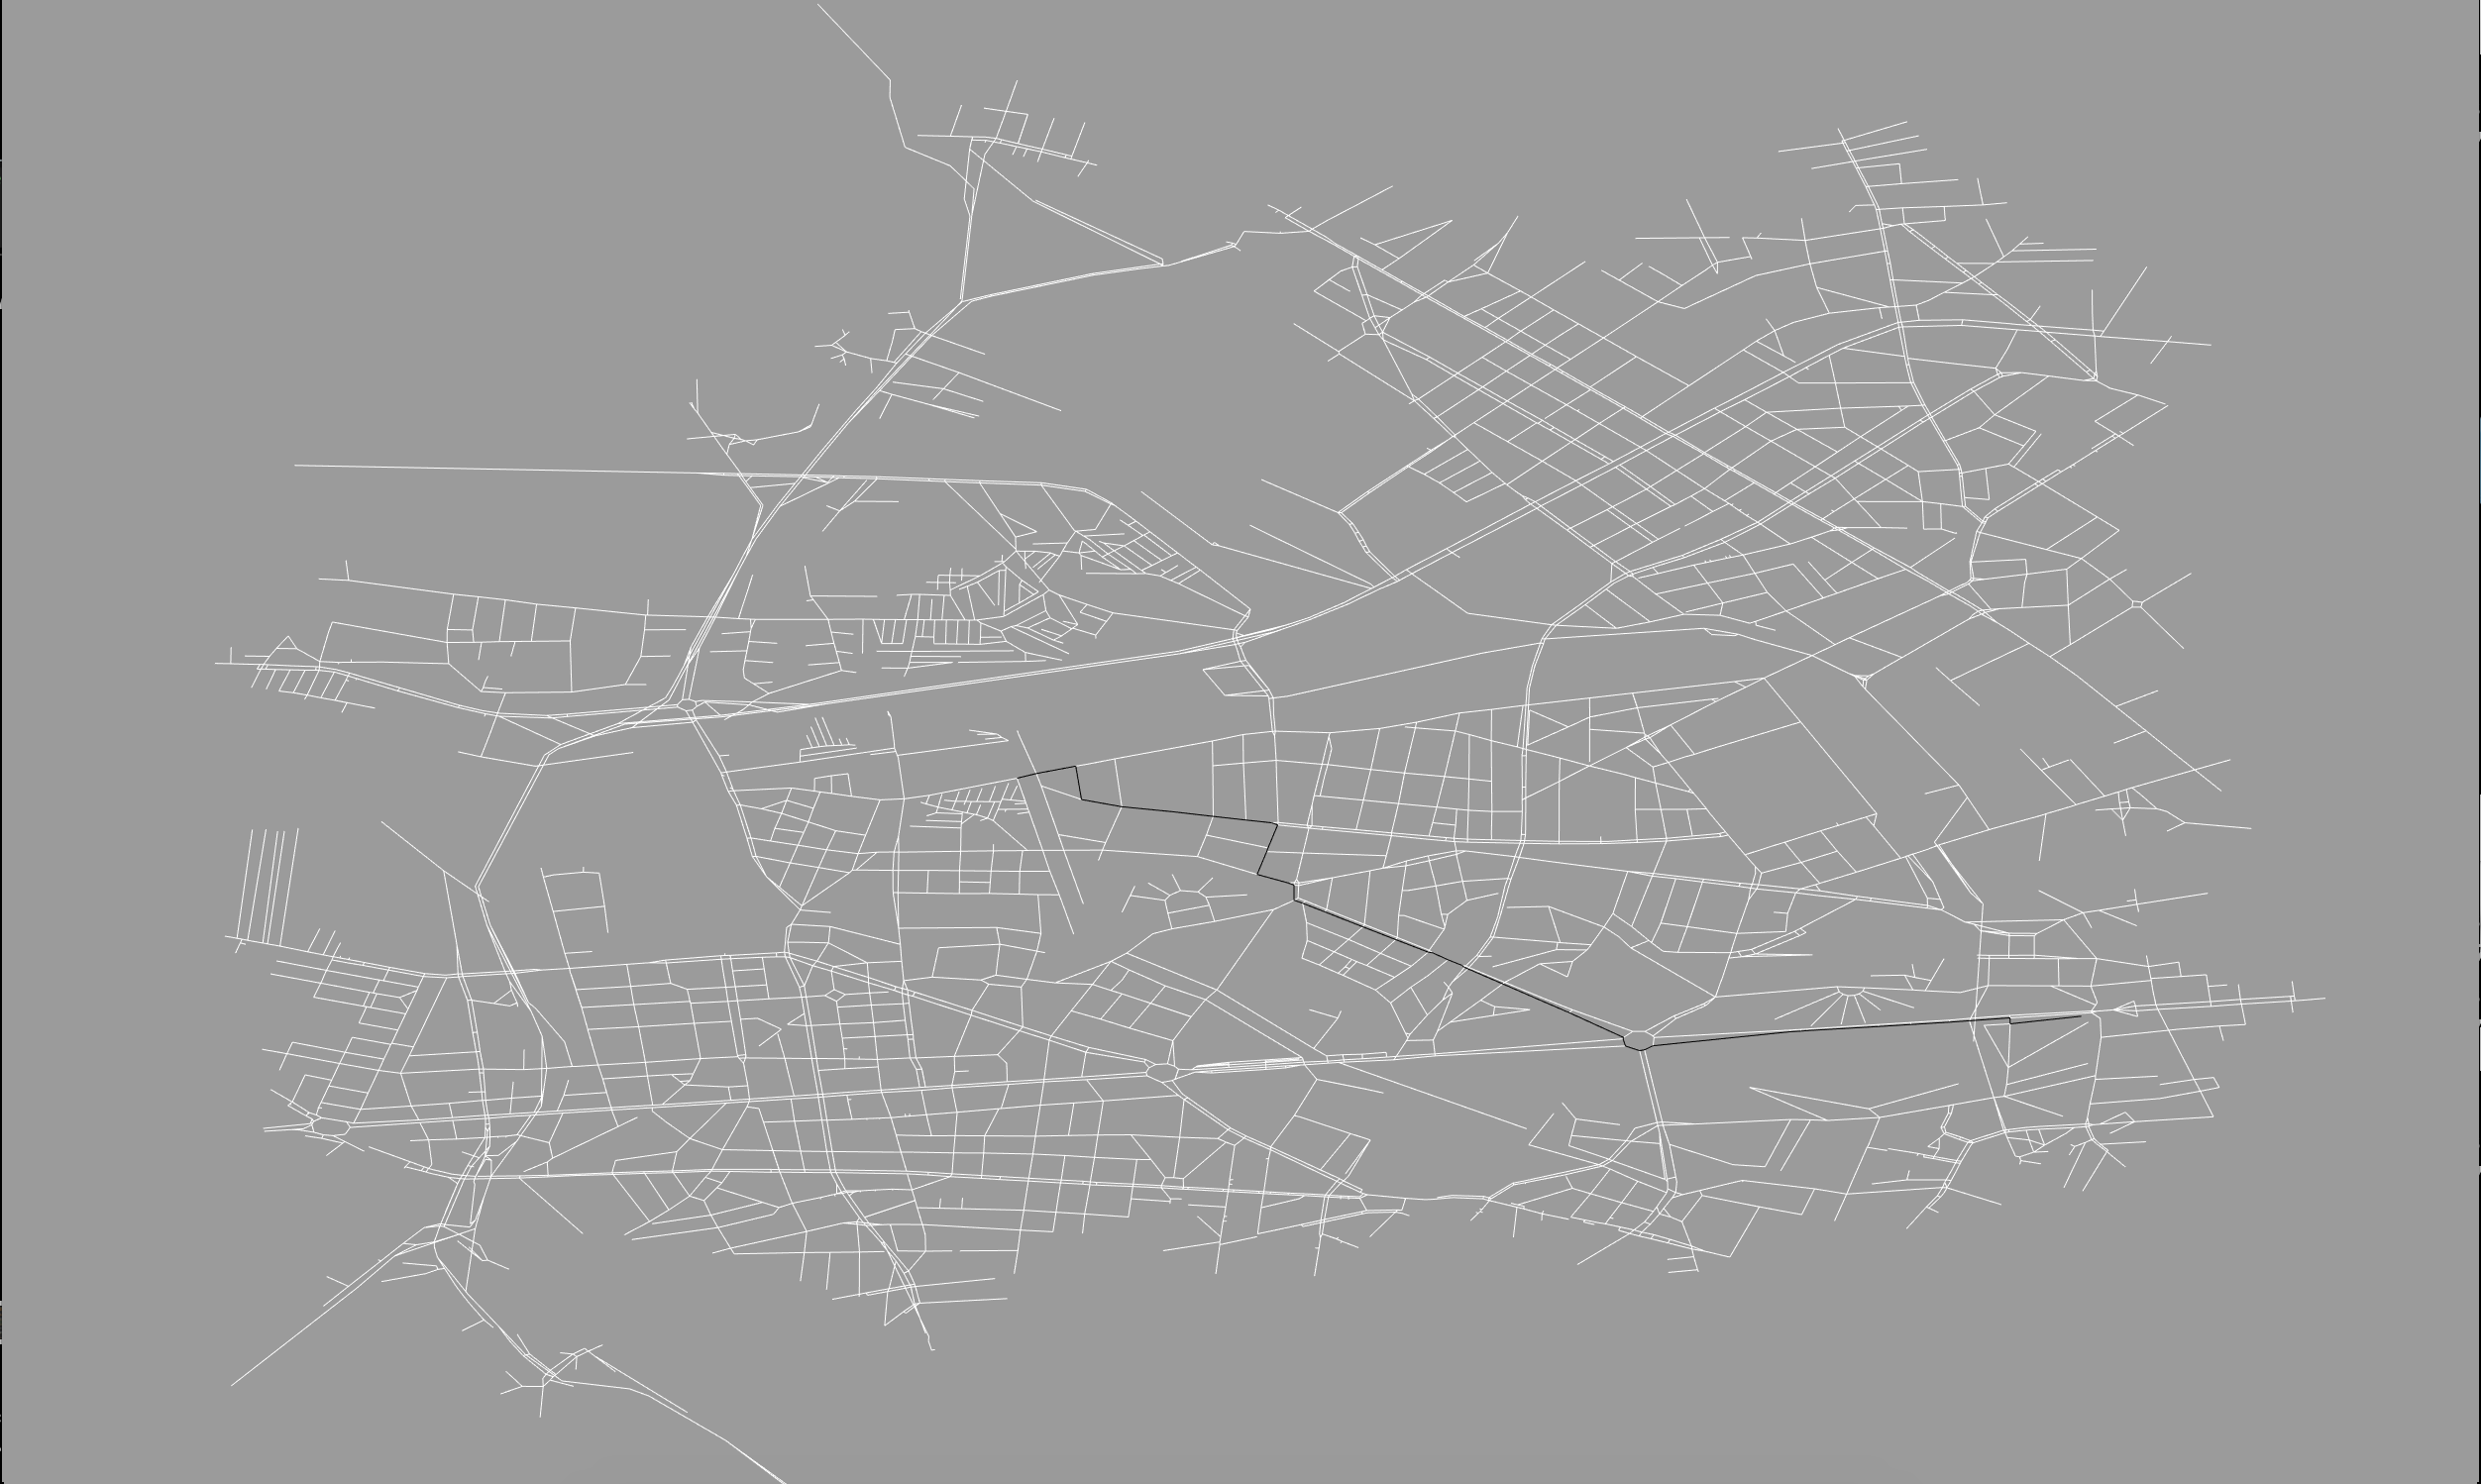
\includegraphics[width=\textwidth]{Images/vis-preprocessing.png}}
\caption[]{Final state of the visualization, using the Preprocessing method on the edge-based visualization.}
\label{fig:preprocessing}
\end{figure}

\Cref{fig:preprocessing} shows a visualization that uses the entire available space on one axis.
As this method is using the same scale on both axes there may be bigger unused space on the other axis.

Based on this we developed another method, that changes the scale on one of the axes to fit the window of the visualization as well.
Therefore, it spreads the graph over the entire screen.

\begin{figure}
    \fbox{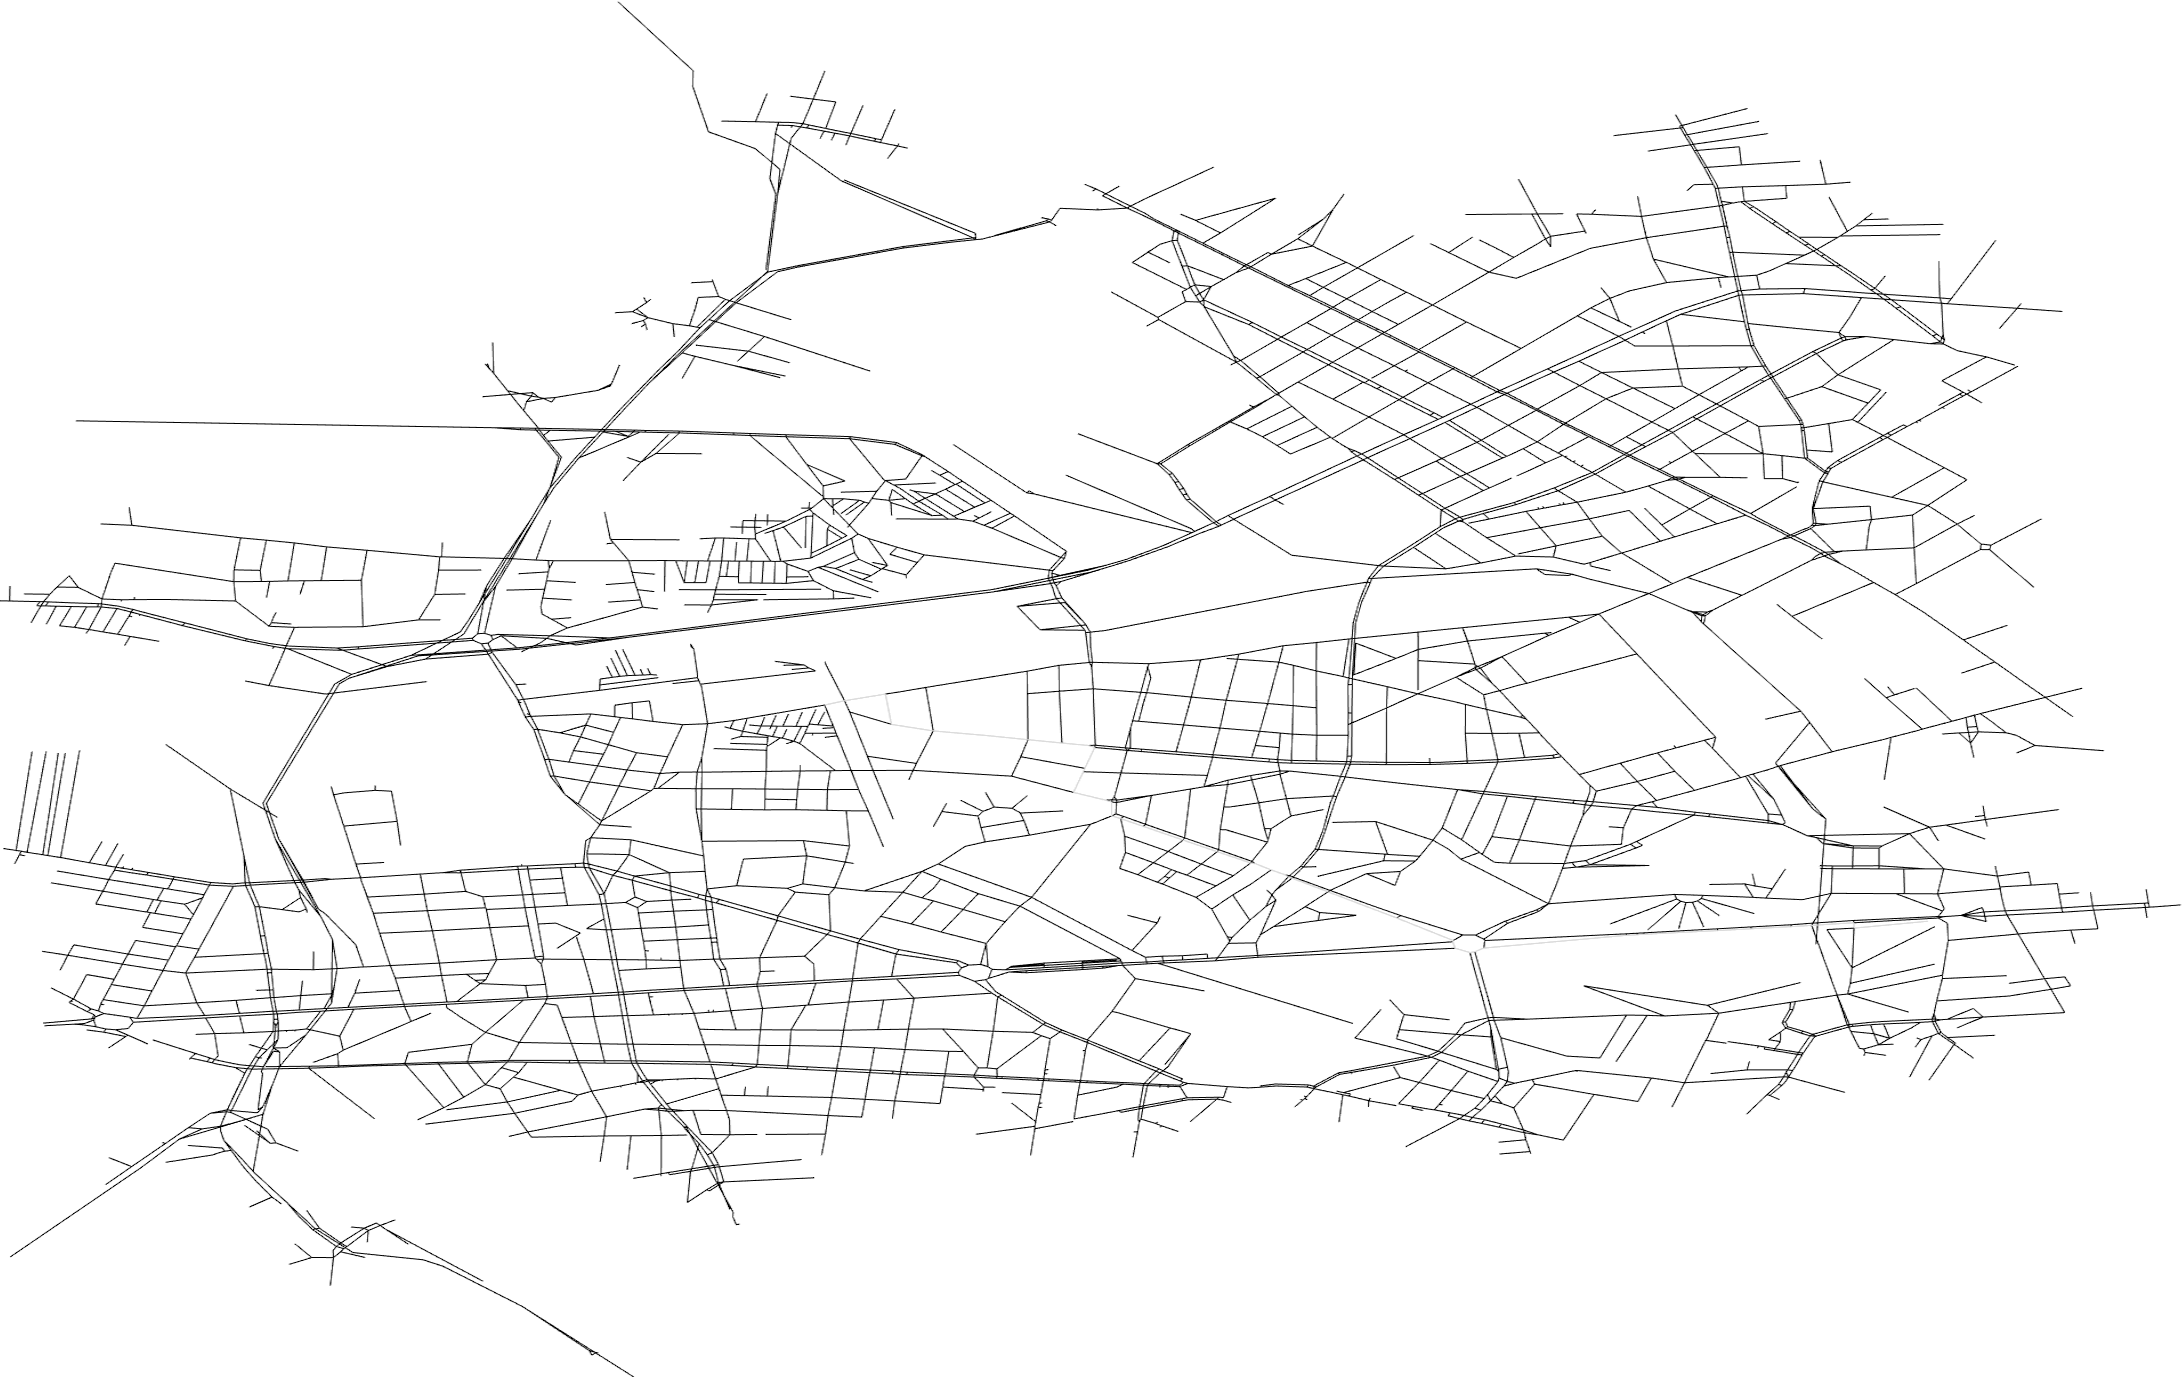
\includegraphics[width=\textwidth]{Images/vis-preprocessing-streched.png}}
\caption[]{Final state of the visualization, using the Preprocessing method with additional streching to the borders of the visualization on the edge-based visualization.}
\label{fig:spreaded_axis}
\end{figure}

As can be seen in \Cref{fig:spreaded_axis} this reduces the unused space to a minimum.
However, we lose a lot of comprehensibility, because the length of a line on the screen corresponds even less to the real edge length.

As a result, we decided to use the preprocessing method with uniform axes for our visualization.
On the one hand, the additional performance costs in preprocessing are worth the reduced amount of unused space.
On the other hand, the possible unused space on one axis is worth the increased comprehensibility.


\subsection{Visualizing the Cache} \label{cache}

In this section, we present a way to display the cache in the visualization.
Taking the tiles as a foundation, we represent the cache by coloring the contained tiles.

\begin{figure}
    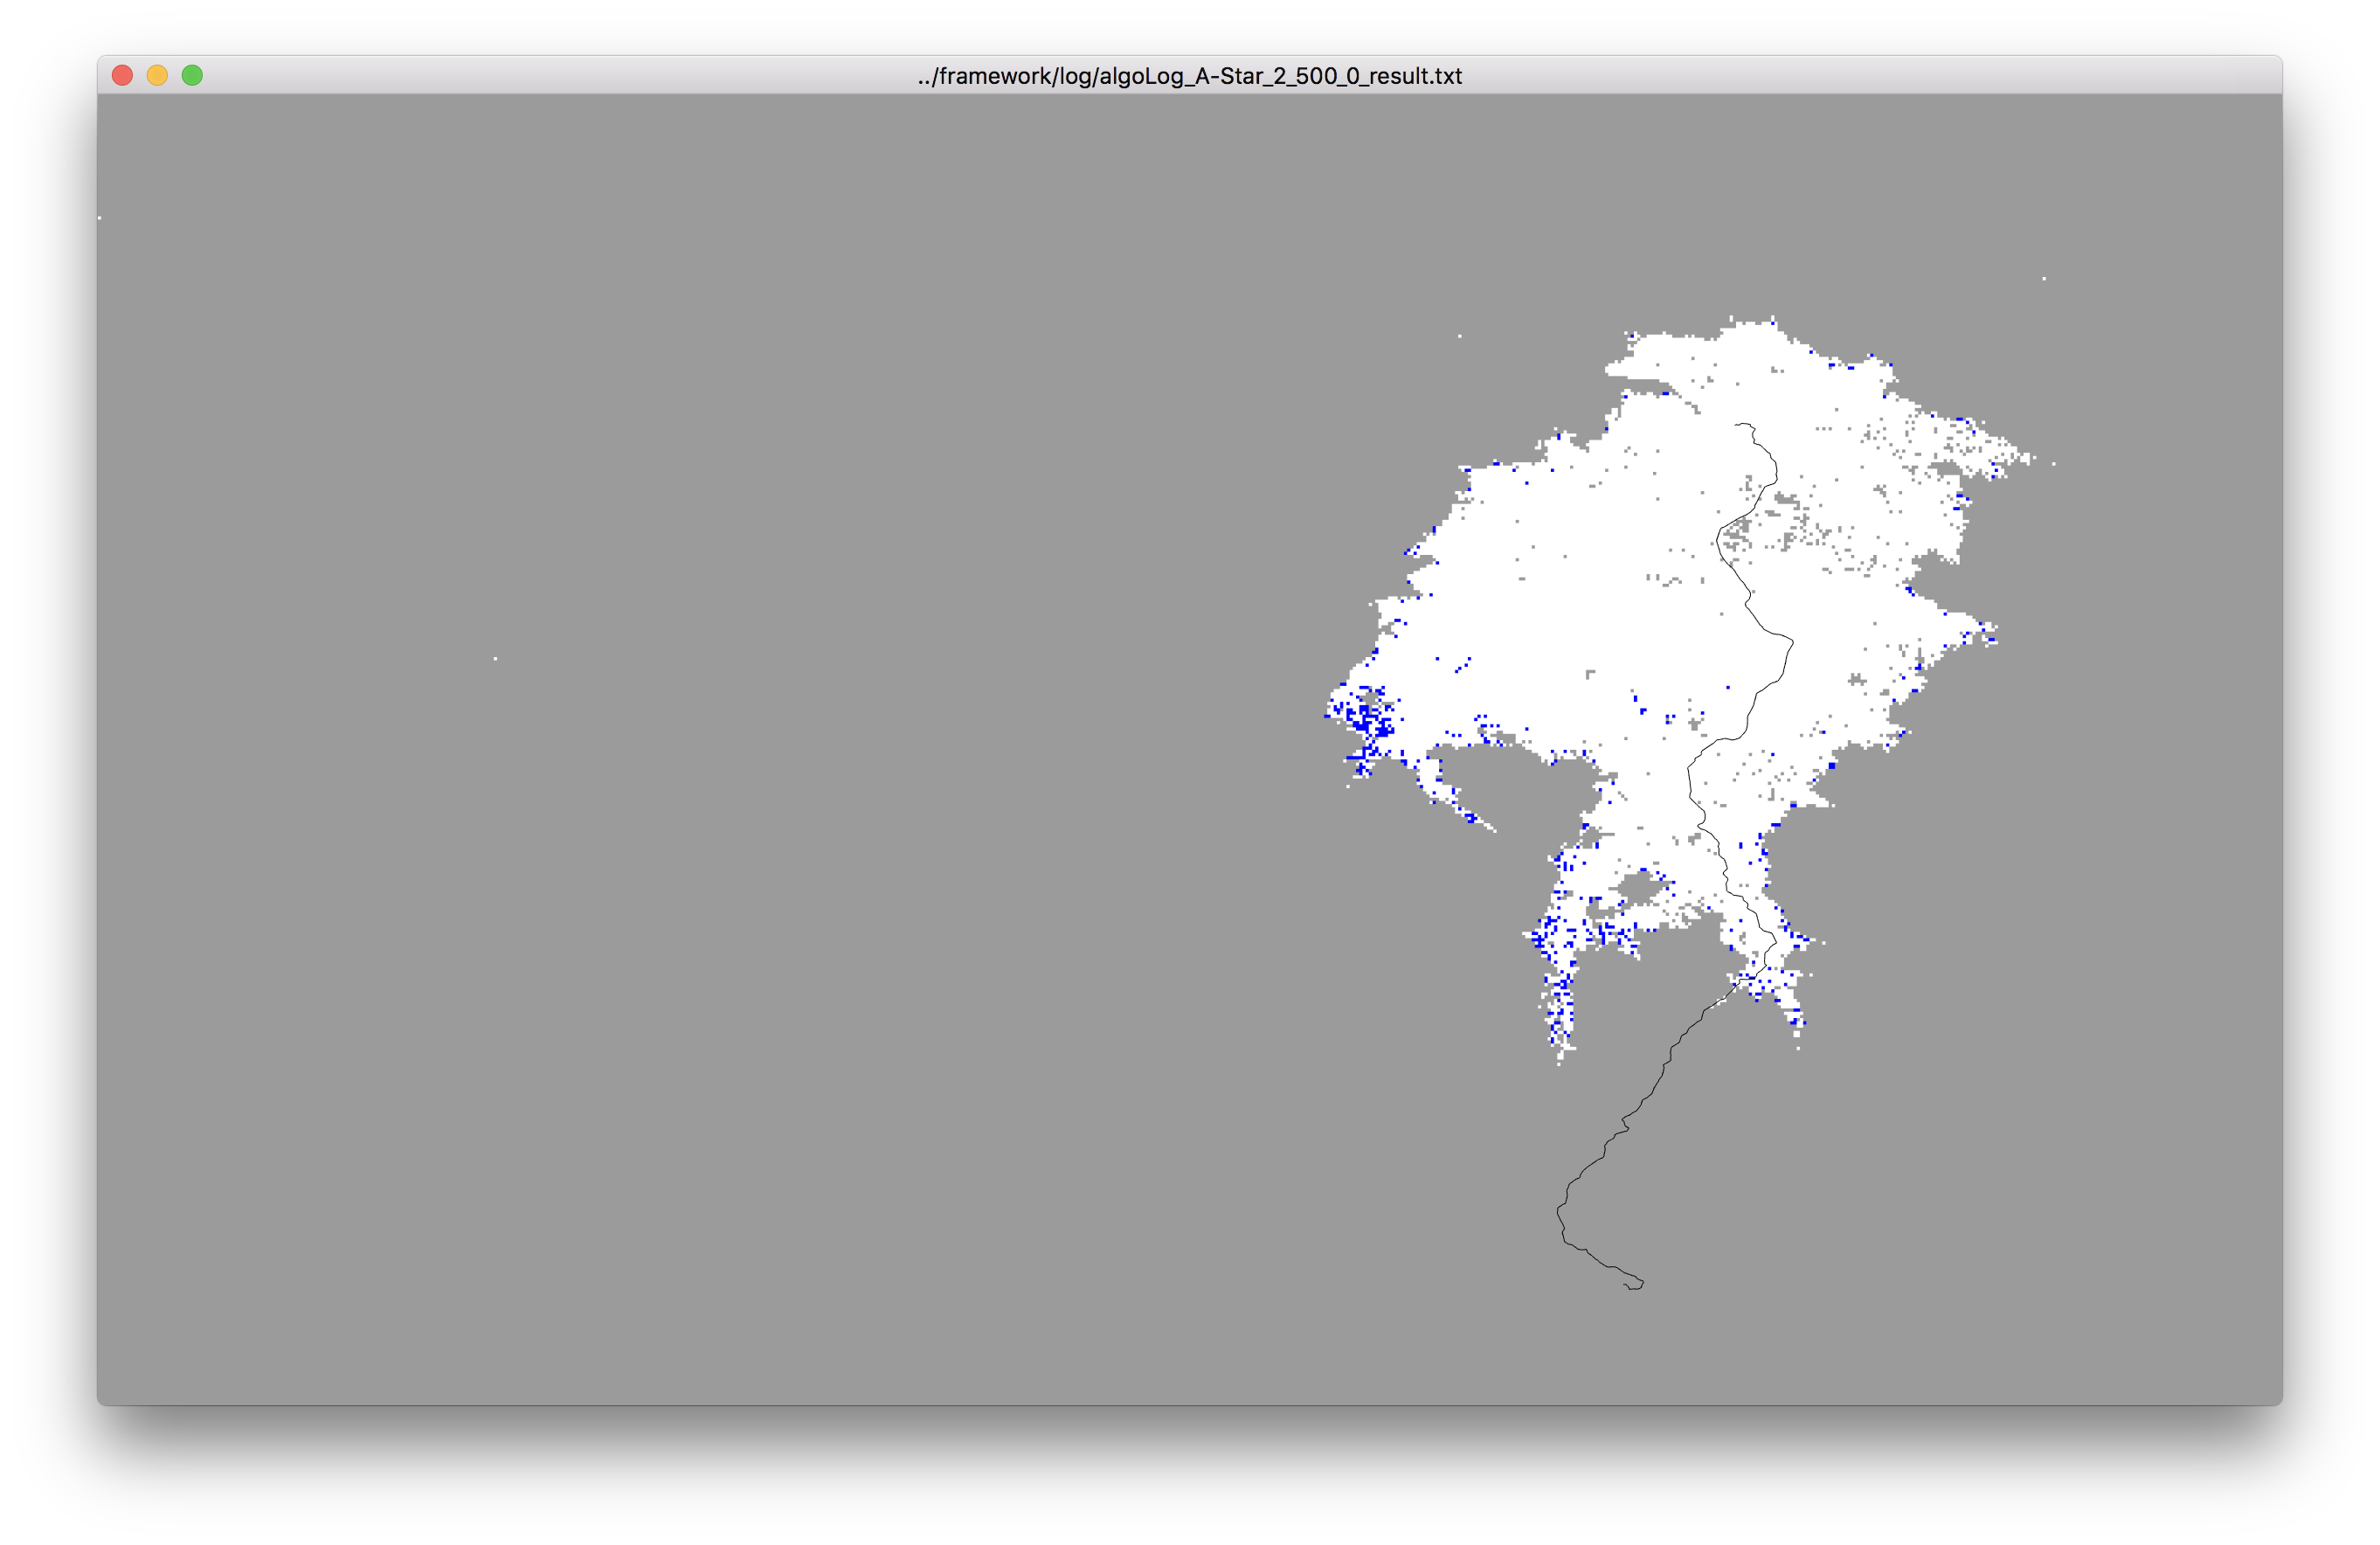
\includegraphics[width=\textwidth]{Images/vis-basic-cache.png}
\caption[]{Representing the cache. The cache is represented by the blue rectangular shapes. The searched path is represented in green.}
\label{fig:cache_coloring}
\end{figure}

In \Cref{fig:cache_coloring} we can see, that we did not color the tiles based on their age anymore.
Due to the colored cache, we achieved an improved understanding of past loaded tiles and the tile-aging would even distract from the important cache.

For showing how well an algorithm performs, we color every tile, whenever it is not in the cache according to the frequency with which it has been loaded.

\begin{figure}
    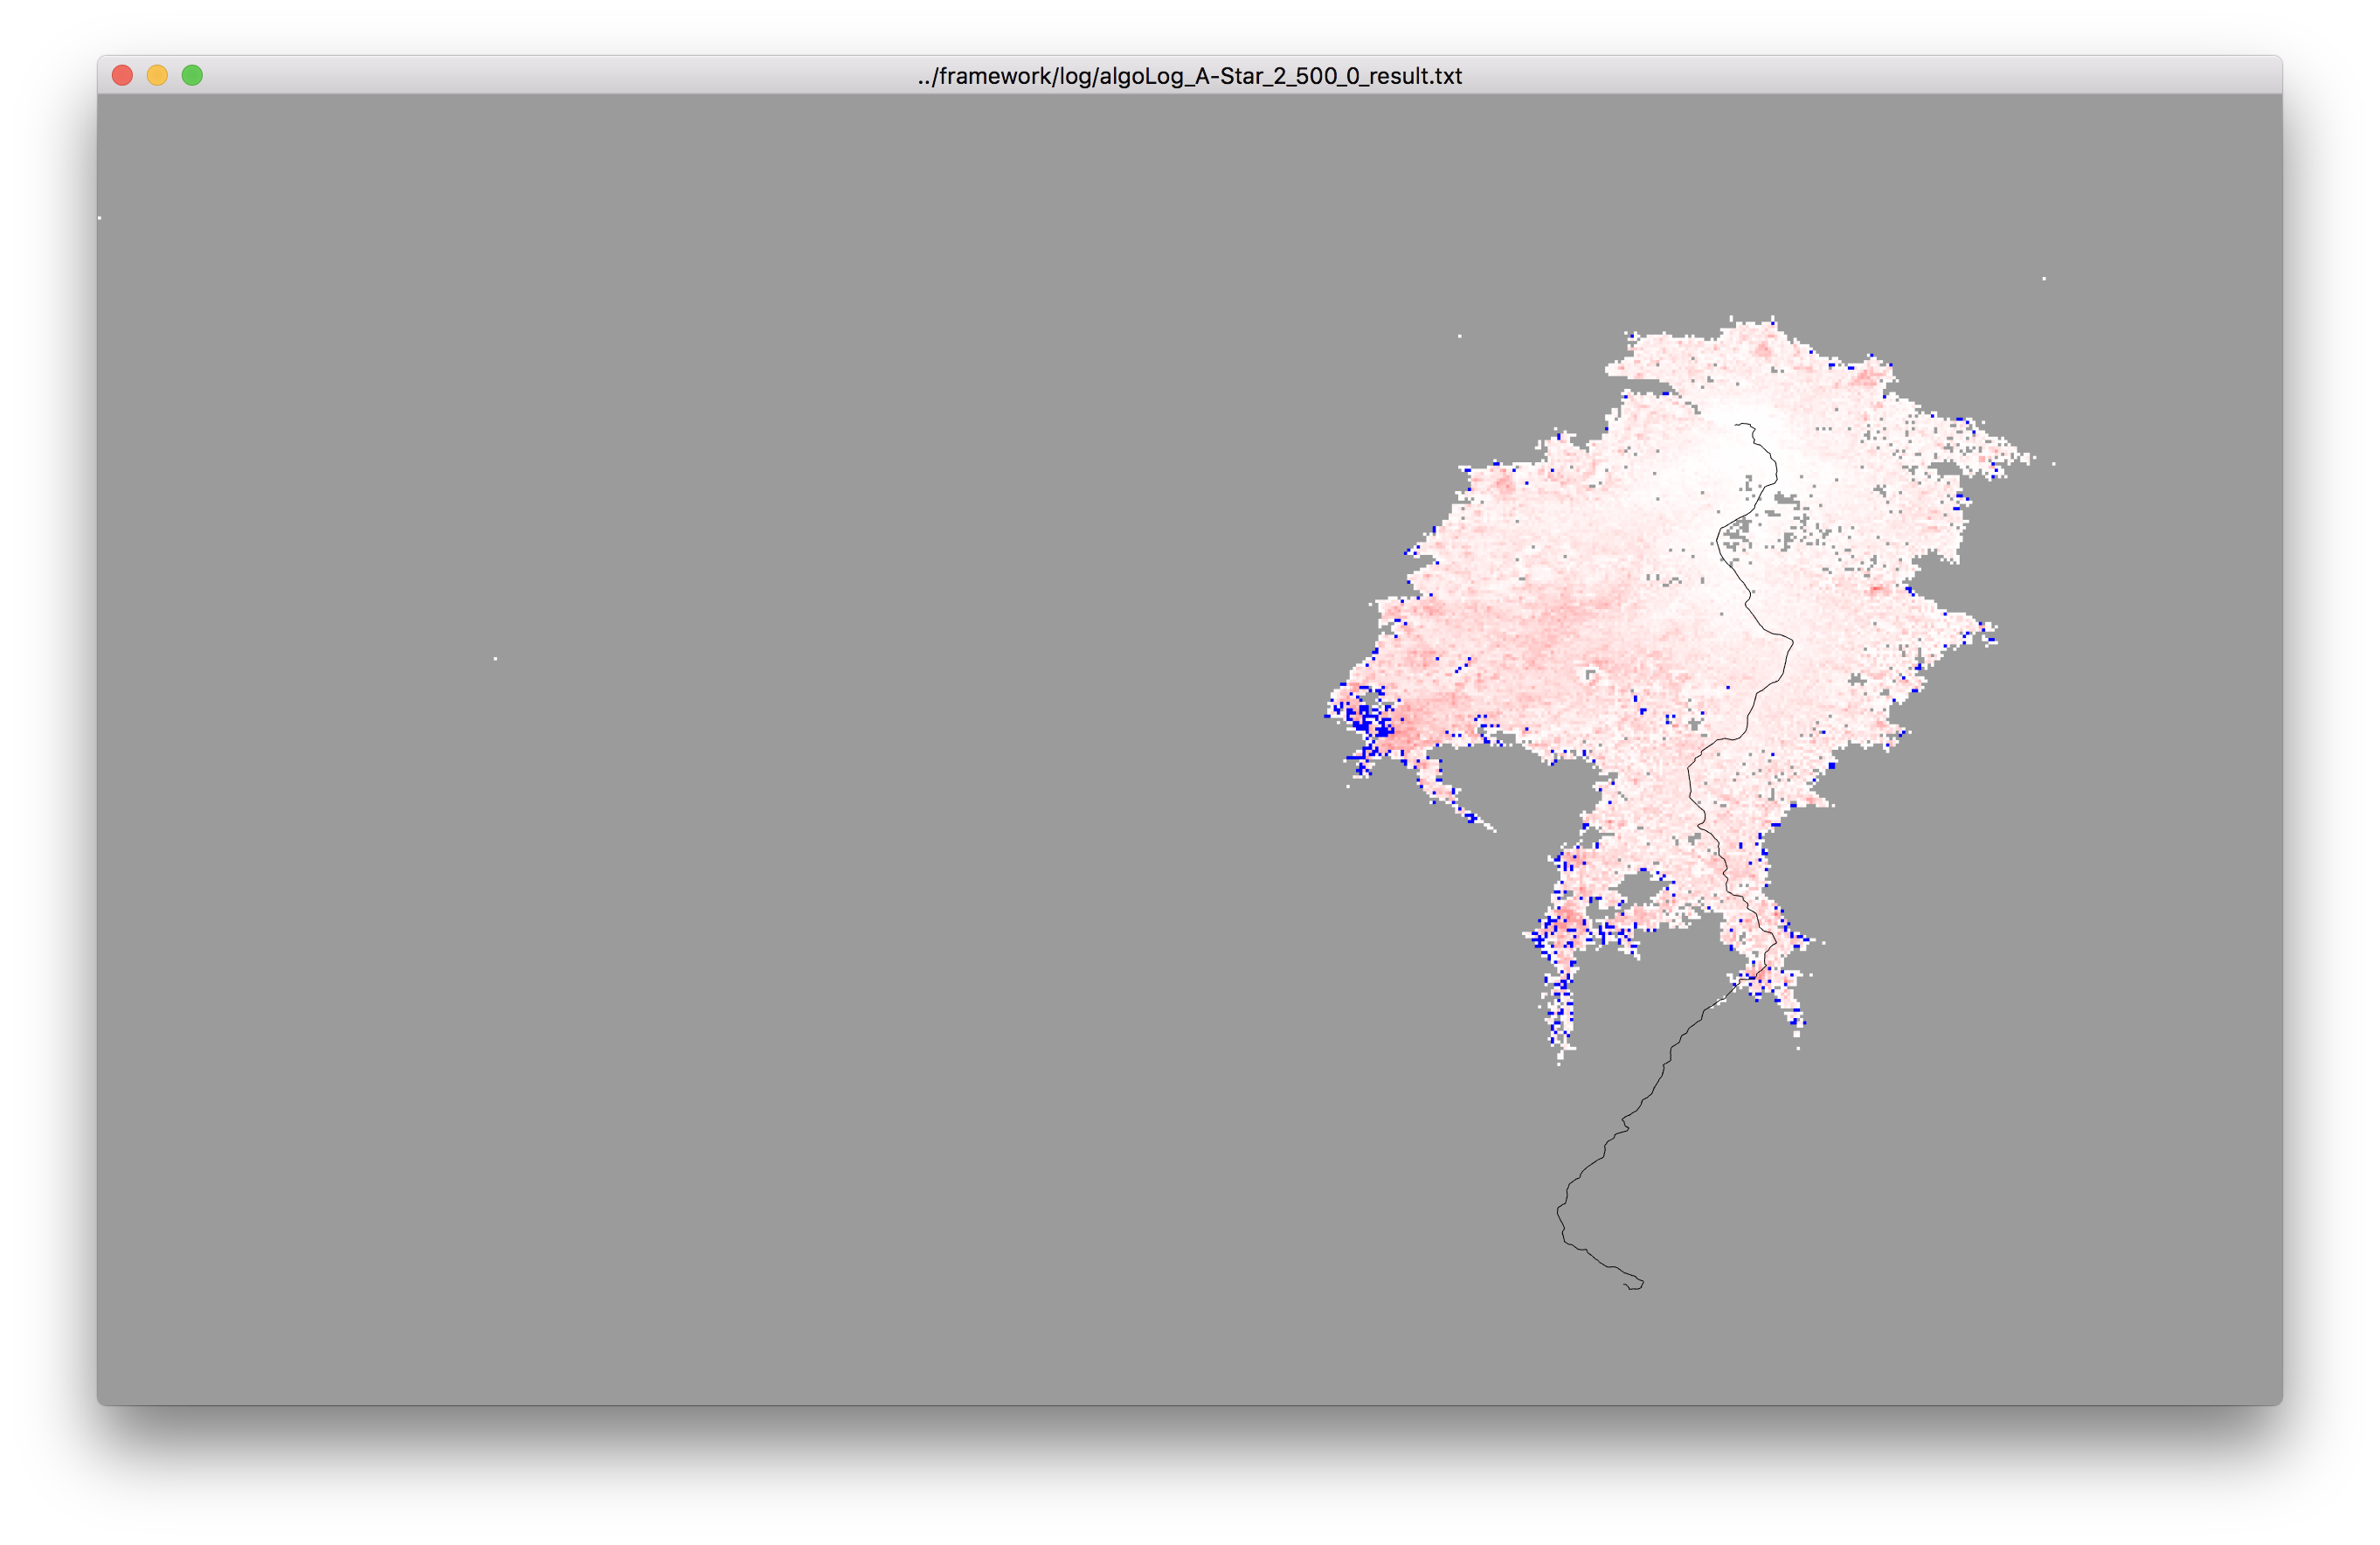
\includegraphics[width=\textwidth]{Images/vis-rgb-cache.png}
\caption[]{Coloring the tiles according to the amount of reloads. Red tiles has been loaded more often. The searched path is represented in green.}
\label{fig:reload_coloring_white}
\end{figure}

By coloring the reloads this way, we can now notice how well our algorithm performs and in which regions more reloads occur.
With this color scheme, bigger differences in tile loading can be distinguished easily.
Nevertheless, smaller differences are difficult to recognize.
Therefore, we tried another color scale.

By using a transition between two colors we hoped to achieve a larger and clearer contrast between slightly different tile loads.
The HSV color space enables us to choose any color as a basis and then adapt the hue linearly according to the amount of reloads.

\begin{figure}
    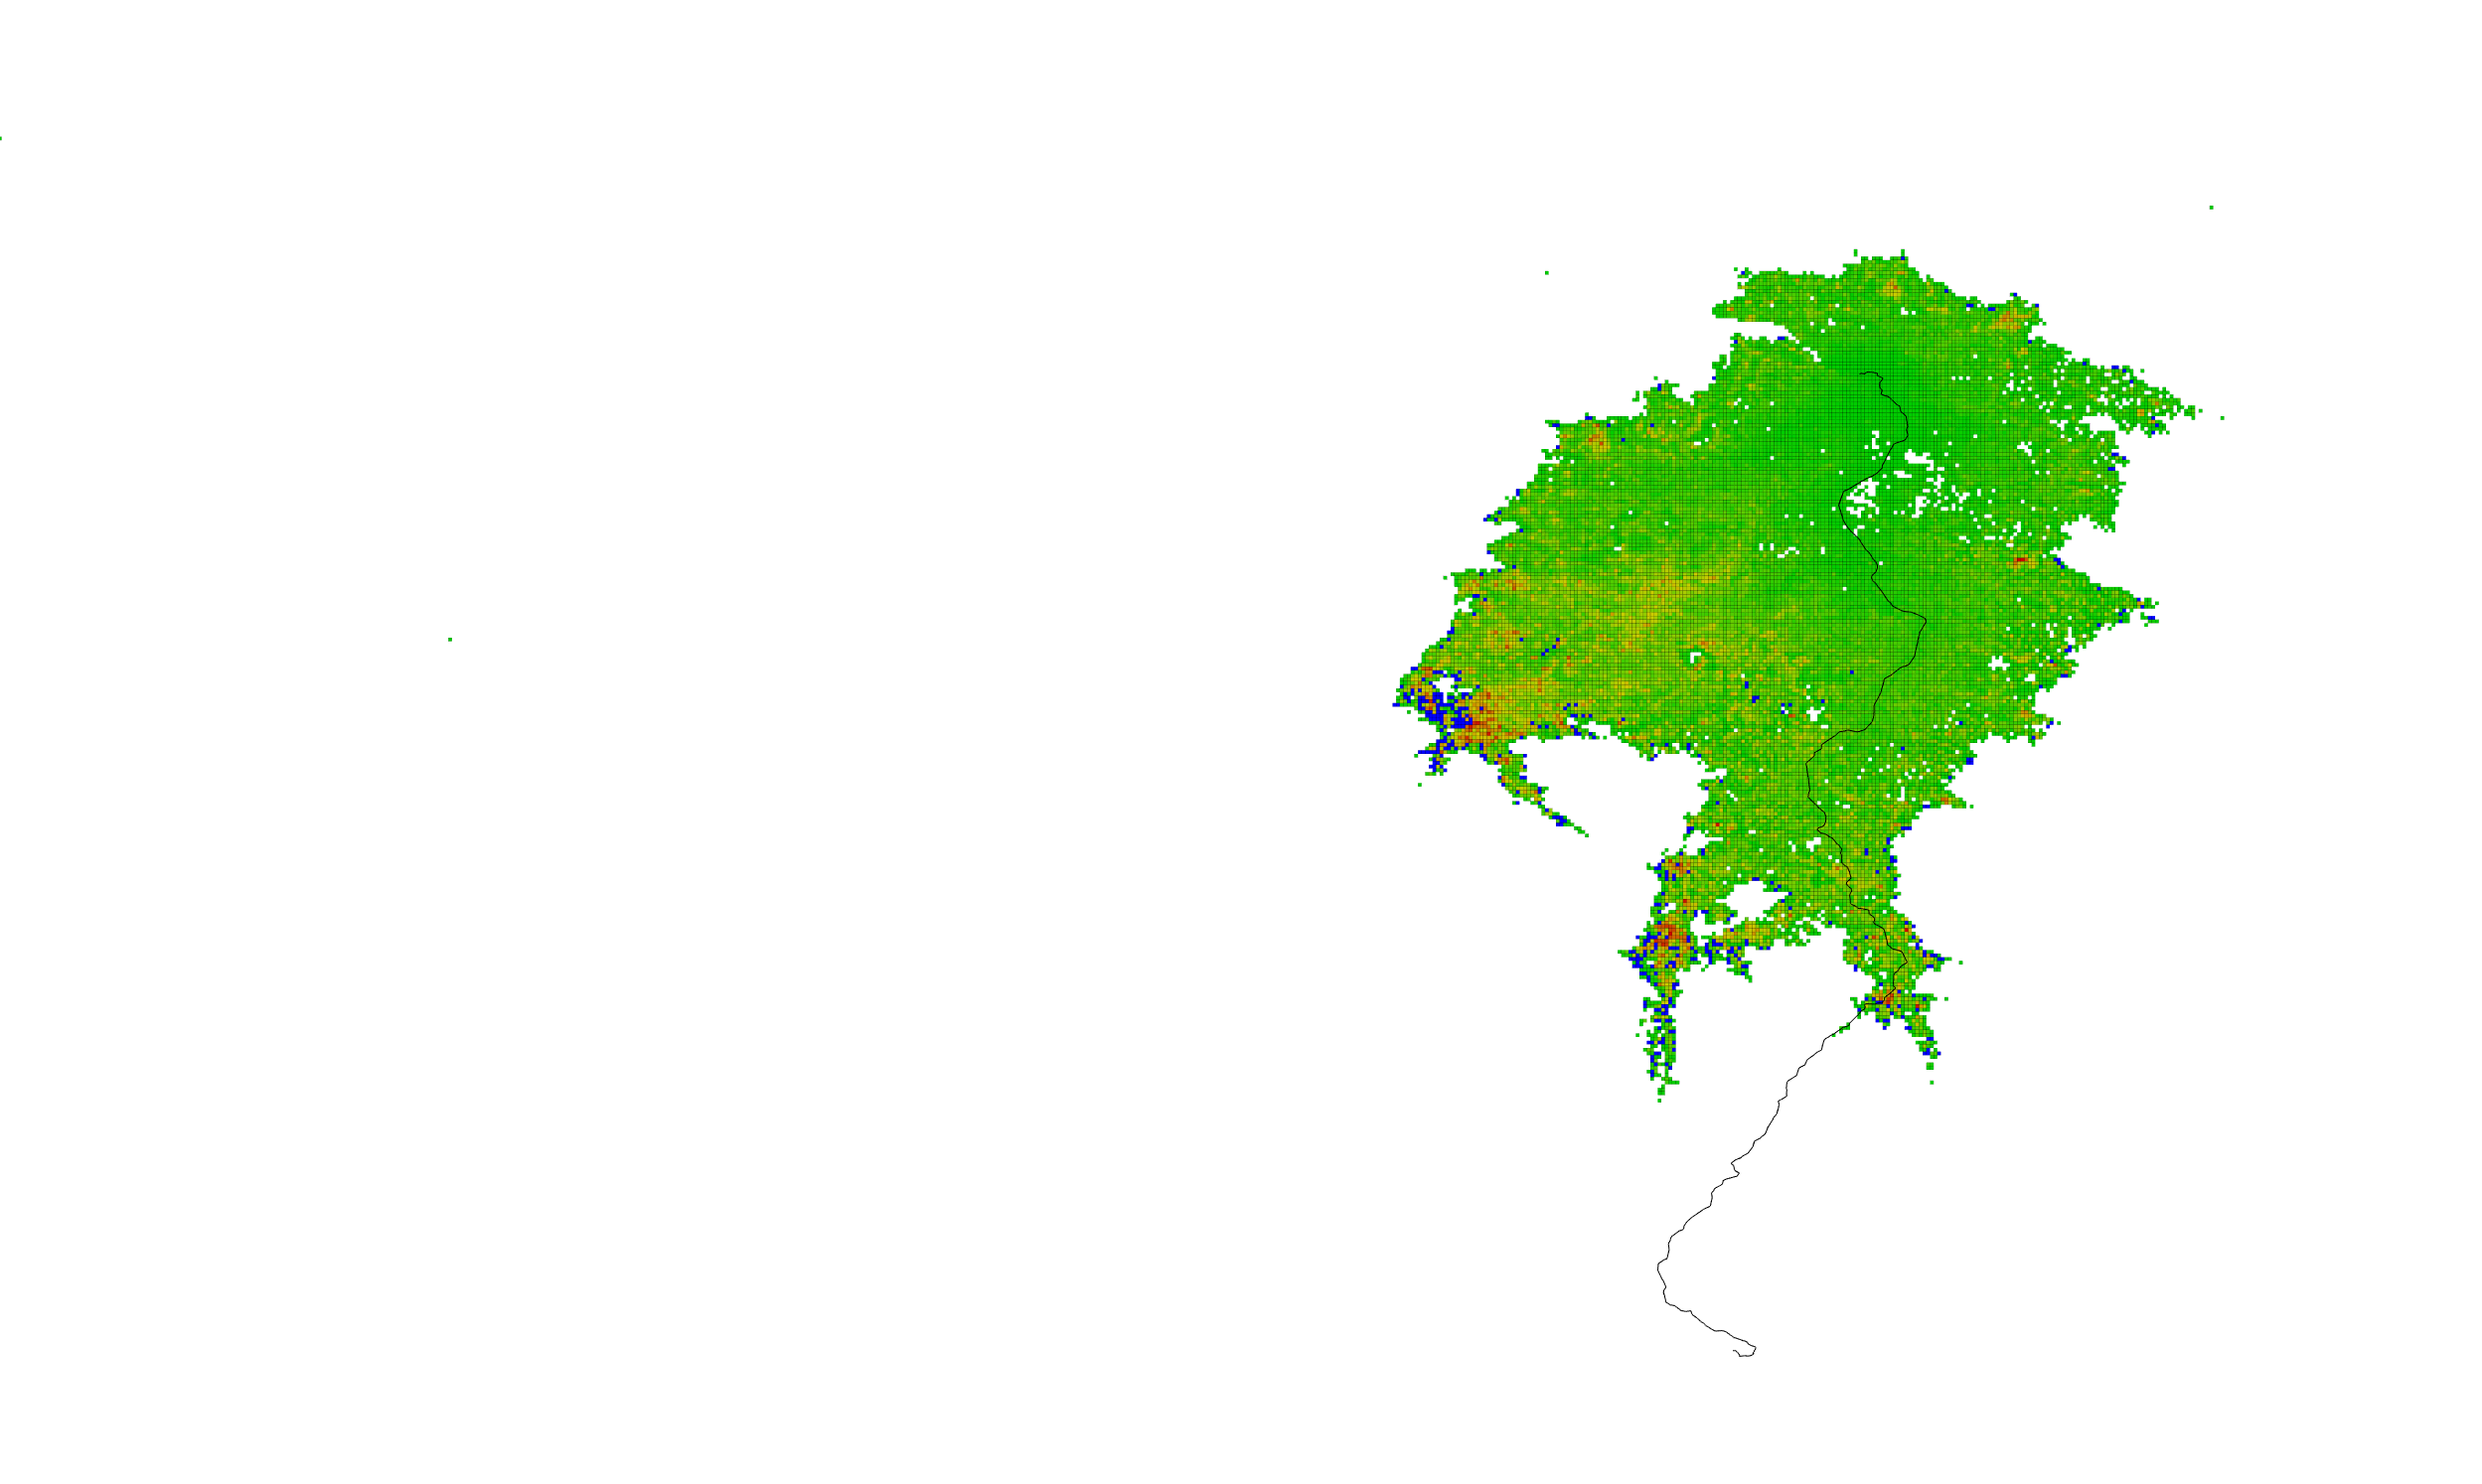
\includegraphics[width=\textwidth]{Images/vis-hsv-cache.png}
\caption[]{Changed color scheme. Now the tiles change their color from green to red. For a better contrast the searched path is now represented in black.}
\label{fig:reload_coloring_hsv}
\end{figure}

In \Cref{fig:reload_coloring_hsv} we notice the differences between two similar values better than during the transition from an uncolored tile to a specific color.
As a side effect, the graph contrasts to the background much better now.

\section{Comparing Algorithms} \label{compare}
A first approach for comparing algortihms is to simply start two visualizations and display in parallel.

\begin{figure}
    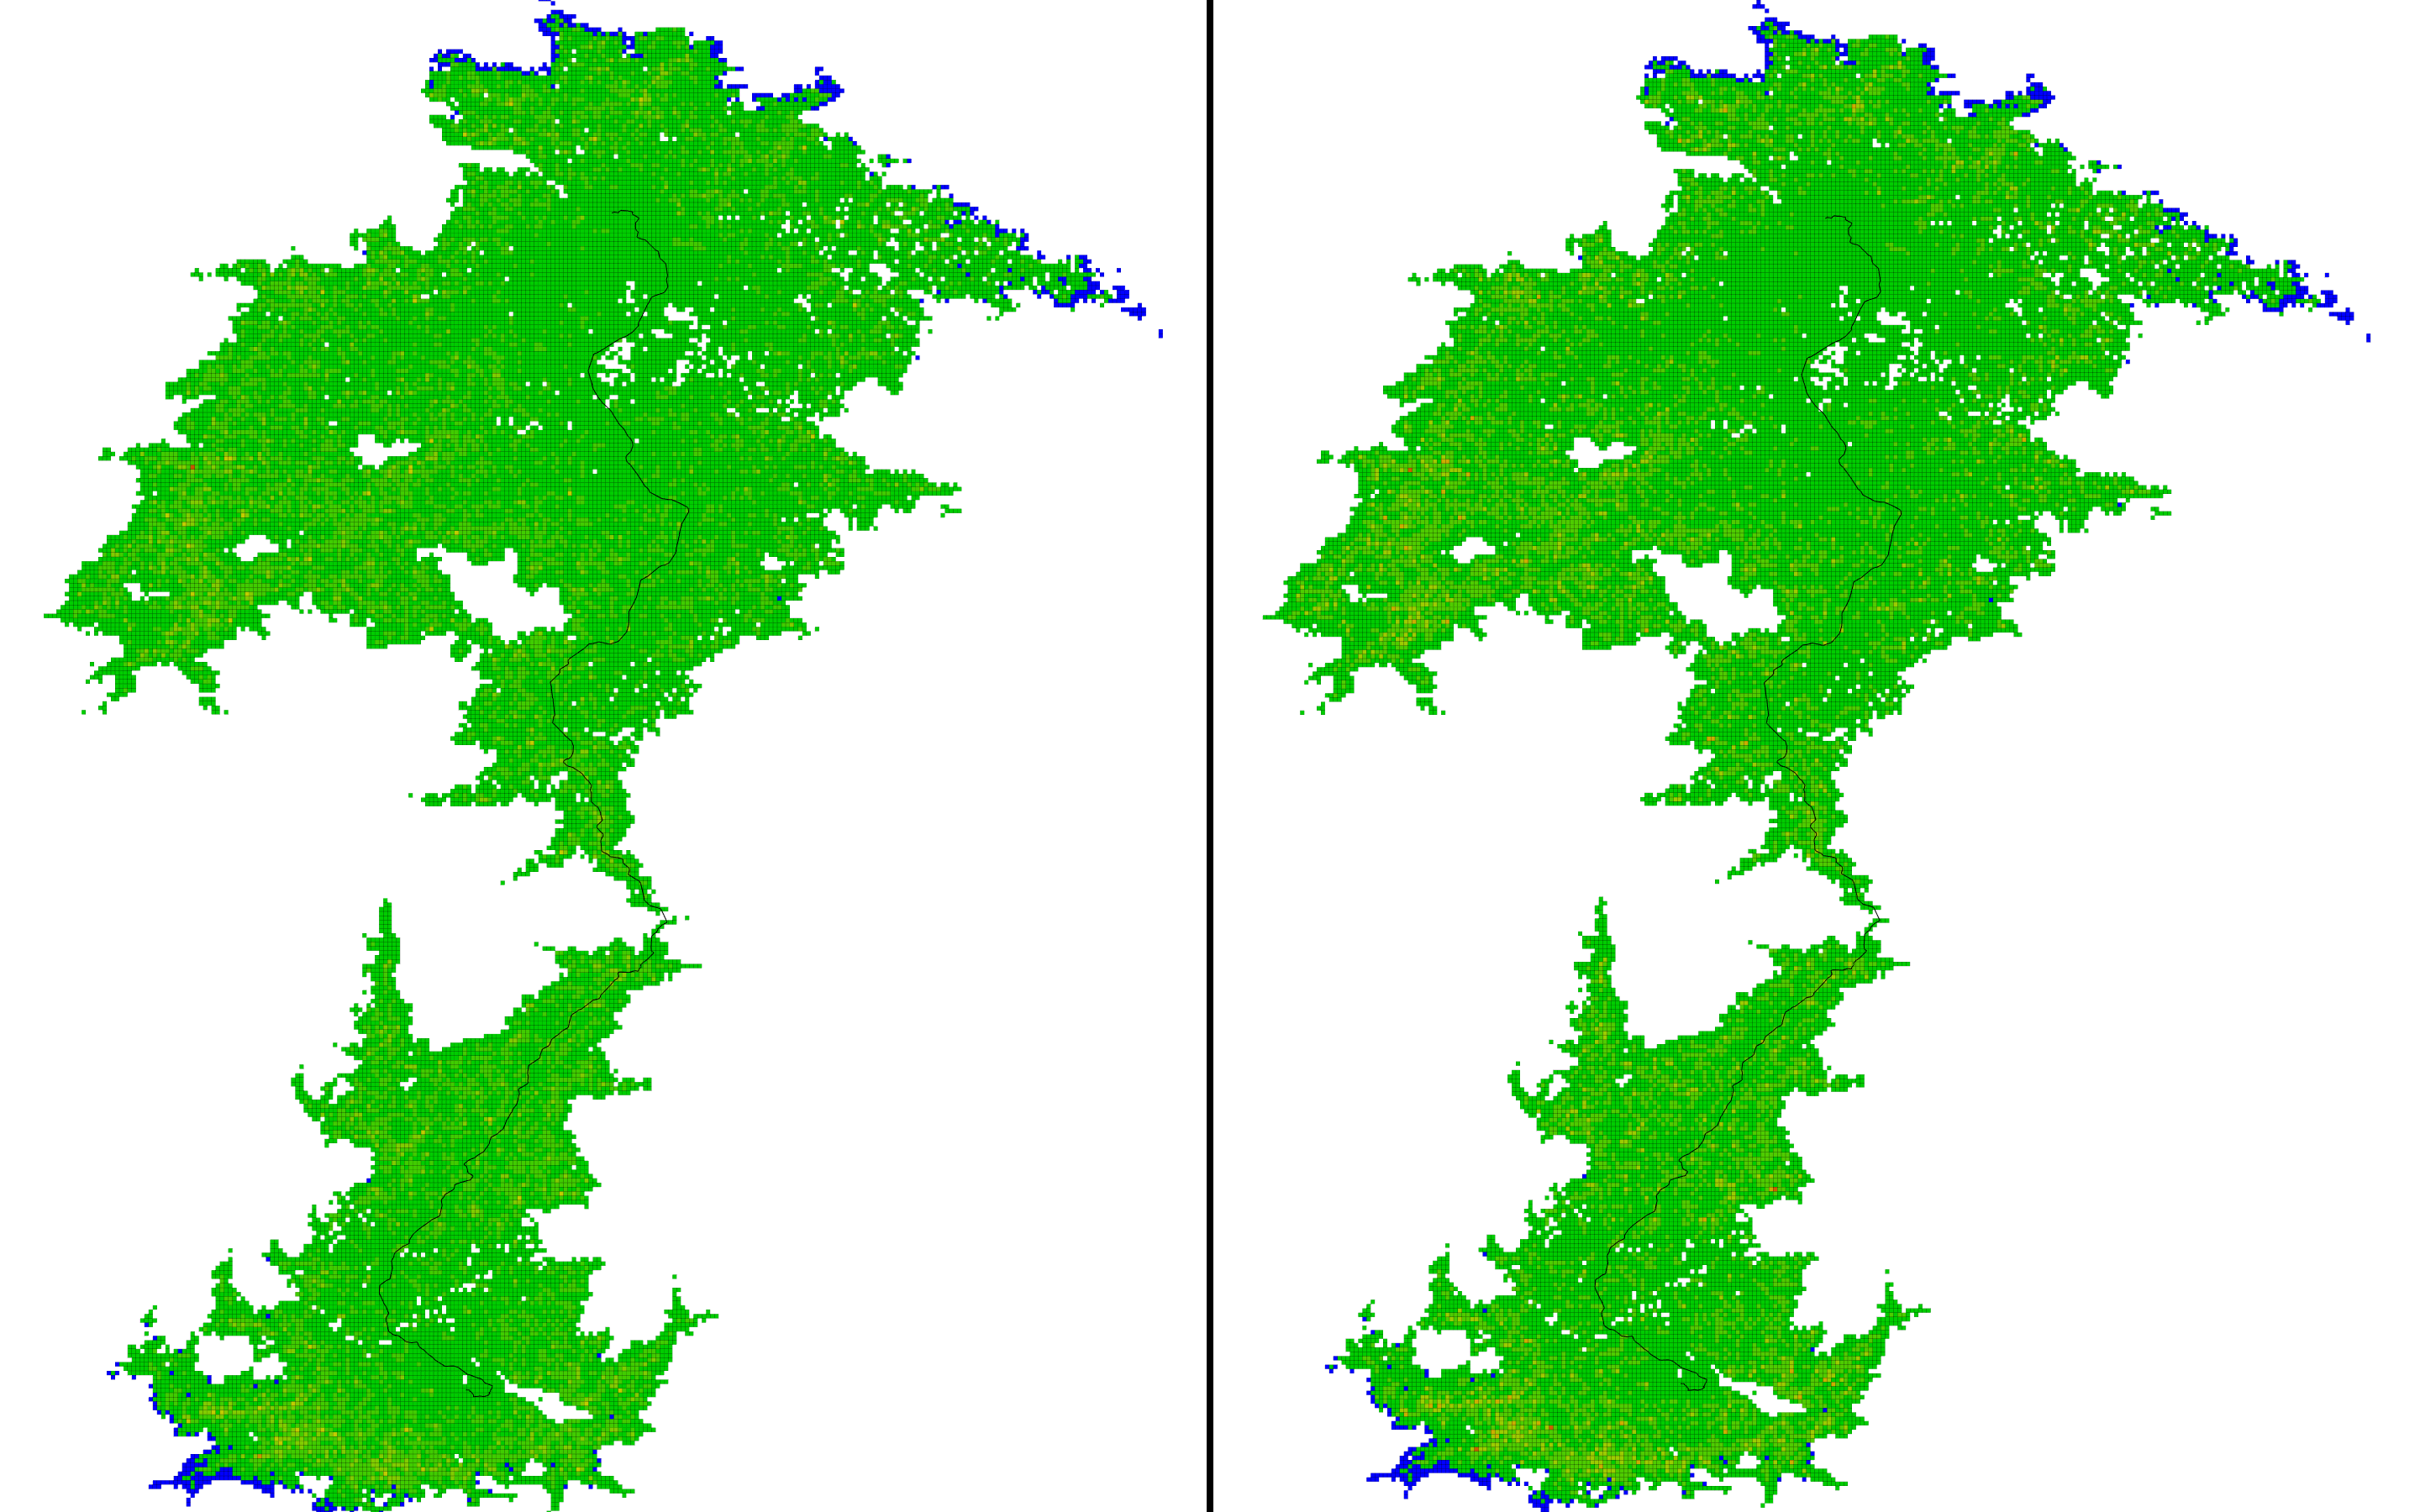
\includegraphics[width=\textwidth]{Images/vis-compare-two.png}
\caption[]{Running two visualizations next to each other.}
\label{fig:two_visualization}
\end{figure}

In \Cref{fig:two_visualization} we can only notice smaller differences in the search space of the two algorithms.
We experienced that this kind of comparison is not useful for really examining differences between algorithms, but for showing them to others.
For really comparing algorithms, we therefore, needed to develop a new variation of the visualization.
Therefore, we removed the space between both visualizations.
The idea is, that smaller differences are more visible, if tiles with the same location are displayed directly next to each other.
Therefore, we split each tile in two and color the left half according to the reloads of one algorithm and the right half according to the reloads of the other algorithm.

\begin{figure}
    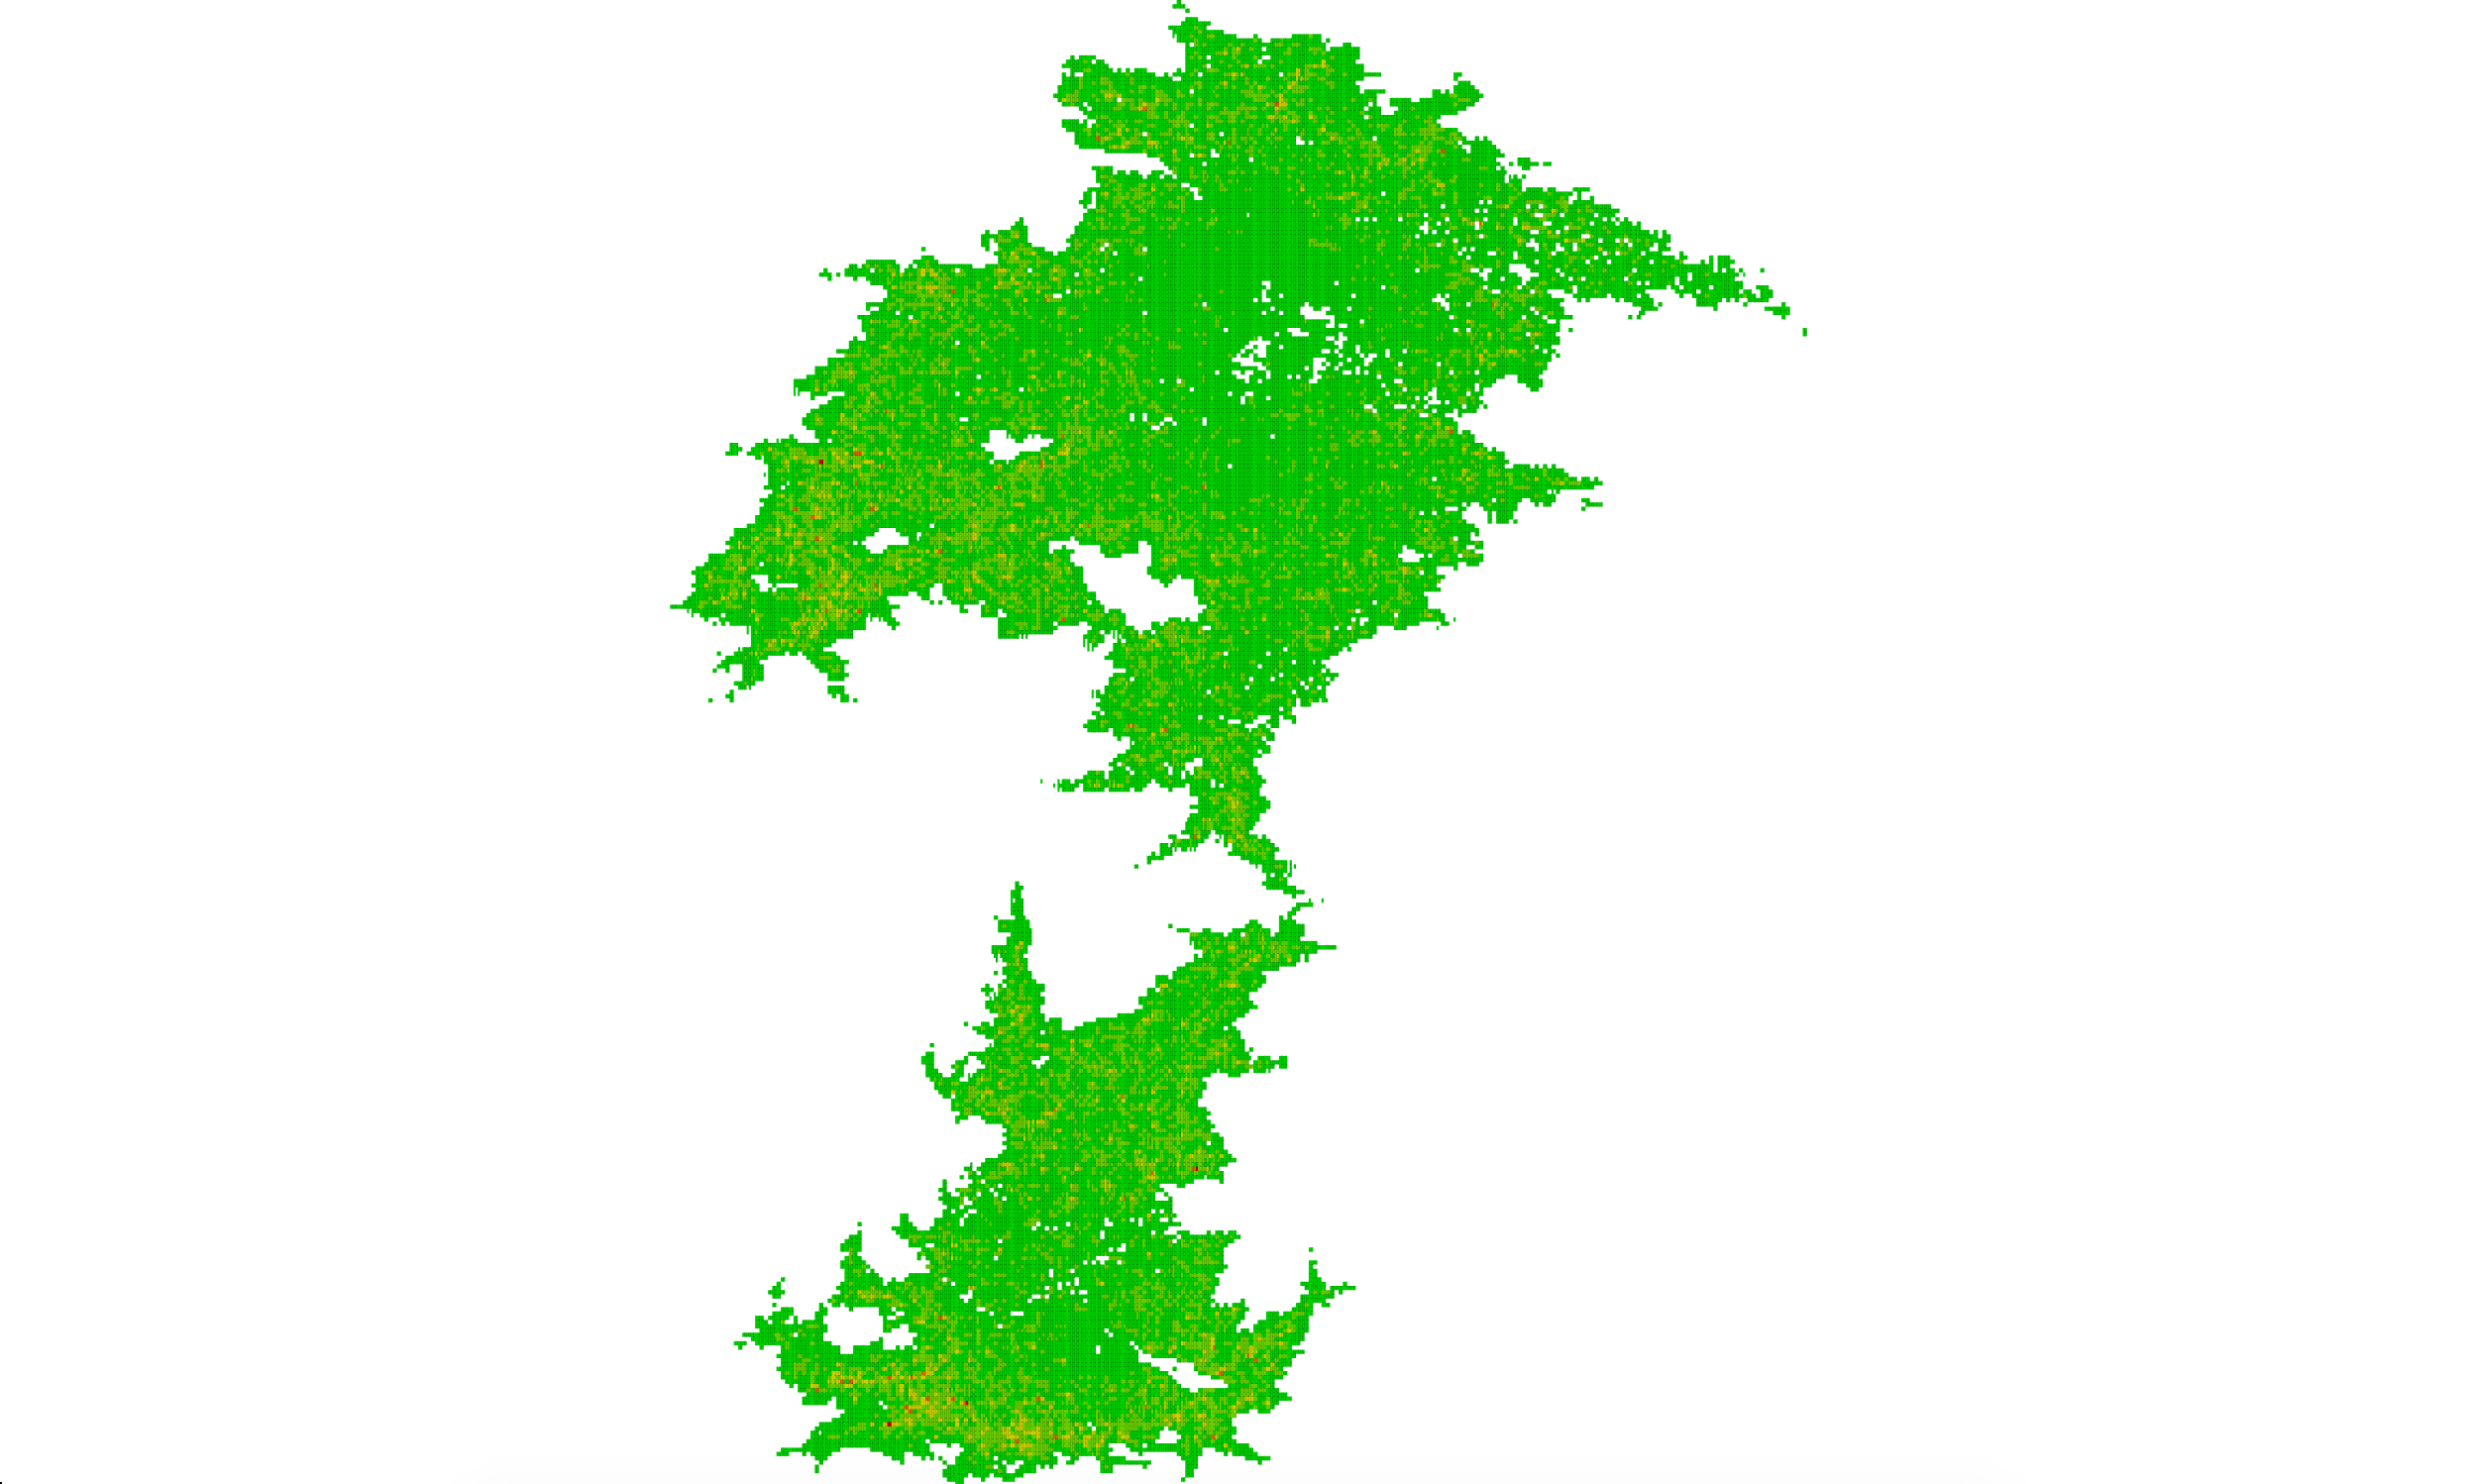
\includegraphics[width=\textwidth]{Images/vis-compare-splitted.png}
\caption[]{Splitting the tiles. The left half of a tile represents one algorithm and the right half the other algorithm.}
\label{fig:splitted_tiles}
\end{figure}

This method provides a better way to emphasize differences on tile level, as we can see in \Cref{fig:splitted_tiles}.
However, it is still difficult to clearly identify differences without longer observation, as it is difficult to associate a tile half to one of the algorithms.
At this point, we could expand this method to label the algorithms with different colored outlines of the tiles, but as we are only interested in the differences between algorithms, when comparing them, we developed an approach that only shows the differences between the tile loads.

This method calculates the difference between the amount of tile loads from both algorithms for each tile.
Then it displays all the tiles that have been accessed by at least one algorithm and colors those blue that have been loaded more often by the first algorithm.
Those that have been loaded more often by the second algorithm are colored red.
The more intense the color, the larger the difference in the amount of tile loads.

\begin{figure}
    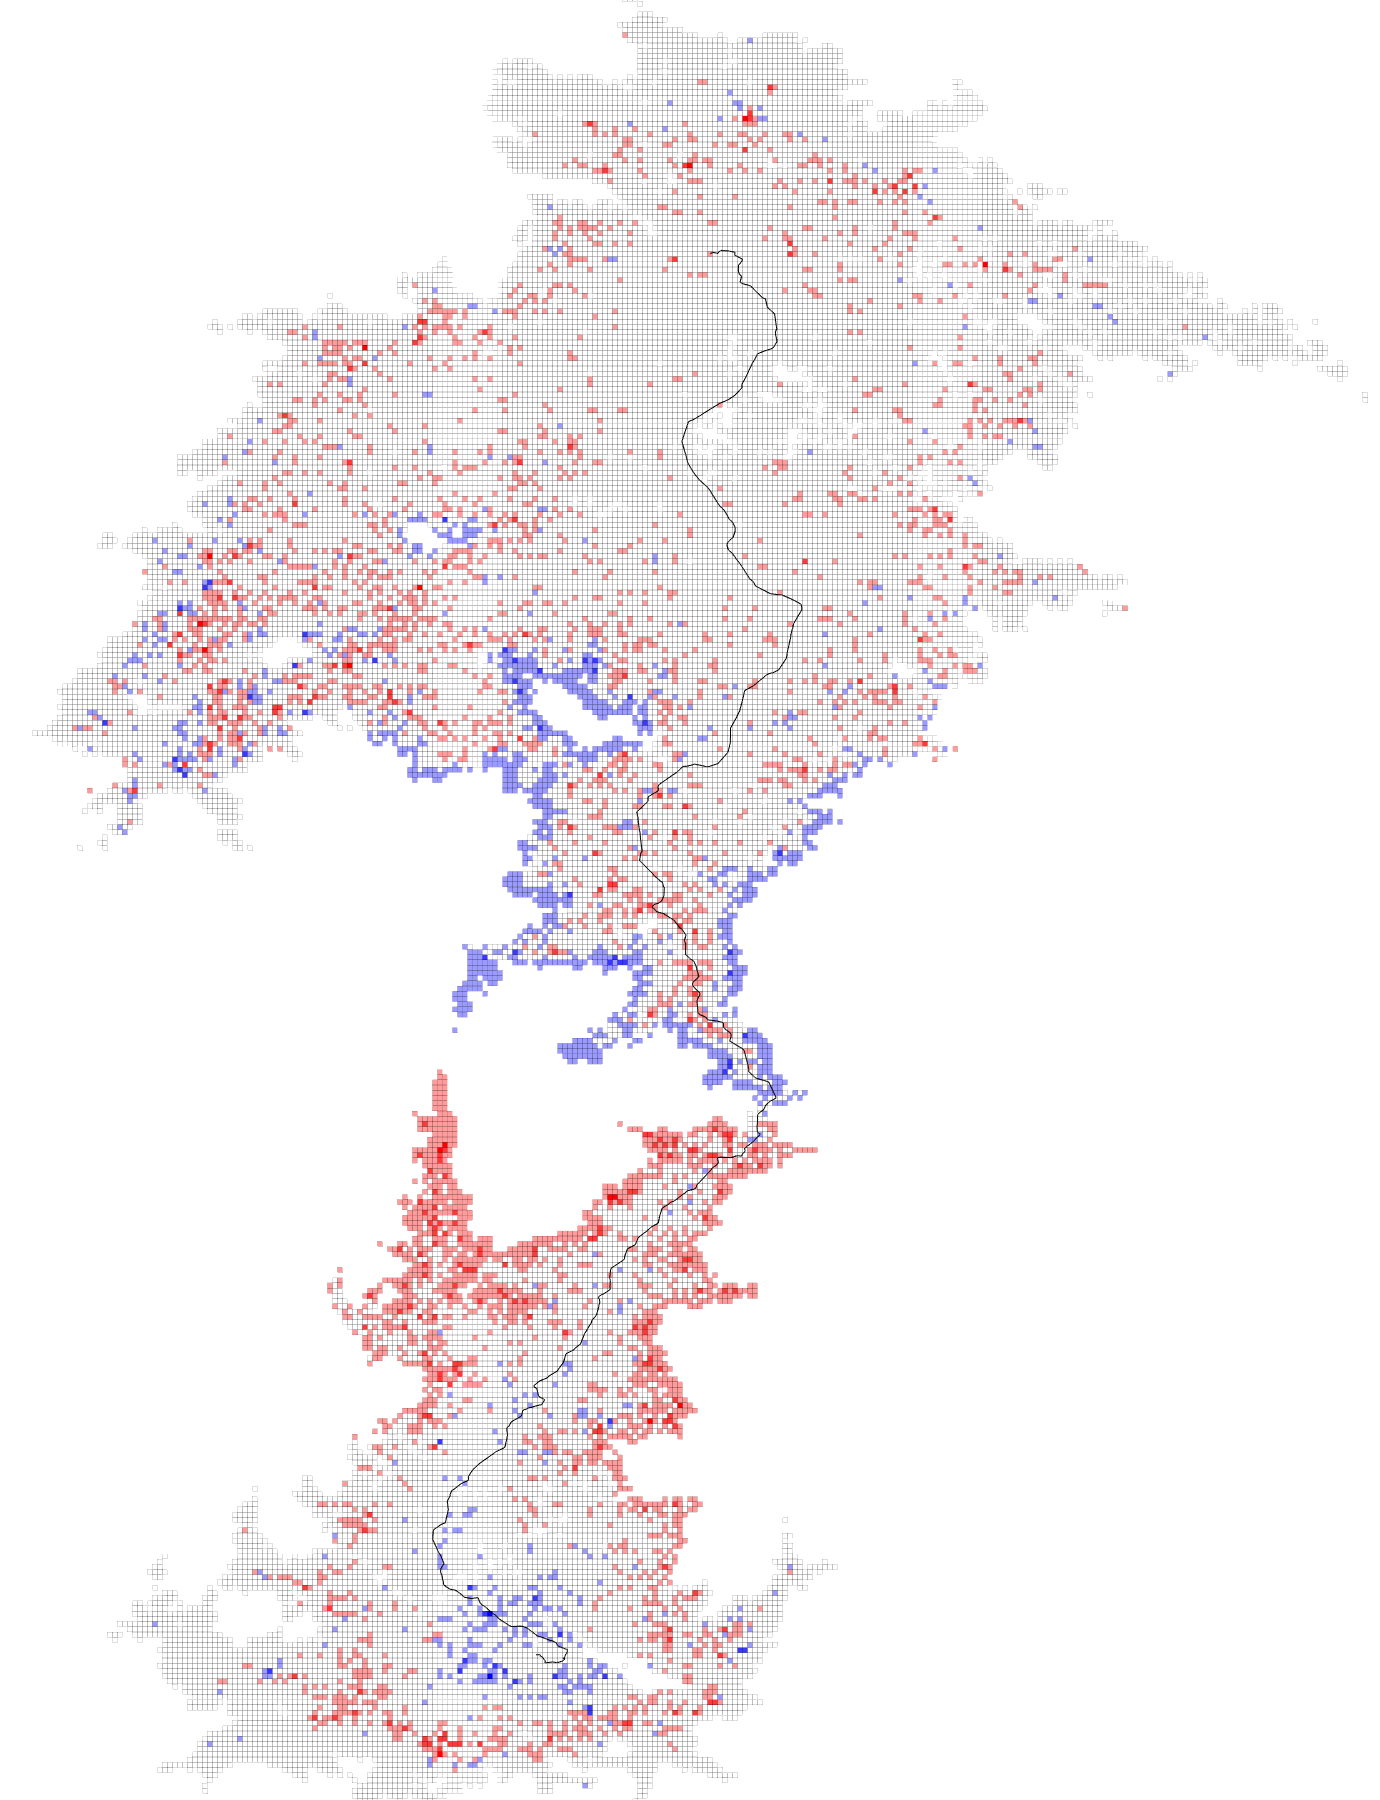
\includegraphics[width=\textwidth]{Images/vis-compare-colored.png}
\caption[]{Showing only the difference of tile loads. Red colors have been loaded more often by the first algorithm, blue colored tiles by the second algorithm. Those tiles colored white, have been loaded equally by both algorithms.}
\label{fig:difference}
\end{figure}

In  \Cref{fig:difference} we can see the comparisson between one algorithm (red) and its variation (blue).
Because of the red and blue bordes of the displayed graph we notice that the search space has changed slightly.
In genereal the visualization has more red than blue tiles and therefore the variation of the algorithm seems to be an improvement in this case.
Apart from the shifted search space there is another area that has a noticeable accumulation of blue tiles around the target in the lower half of the visualization.
After a closer look at this we discovered that when the affected area is explored the cache is mostly used for tiles in the upper part of graph.
This leads to further reloading in the lower part.
Hence, we were able to fix this error pattern and made the cache available when it was needed in the lower part.


\section{Miscellaneous}

In this section, we will take a look at the visualization we have just built and present some additional features.
For longer routes, as can be seen in \Cref{fig:reload_coloring_hsv}, we had to realize, that even the visualization, that displays only the tiles, has a problem in that single elements, in this case the tiles, become quite small.
Therefore, we added a zoom feature to the visualization.
After having included this feature it was necessary to enable panning as well, otherwise we could only examine the middle of the graph.

\begin{figure}
    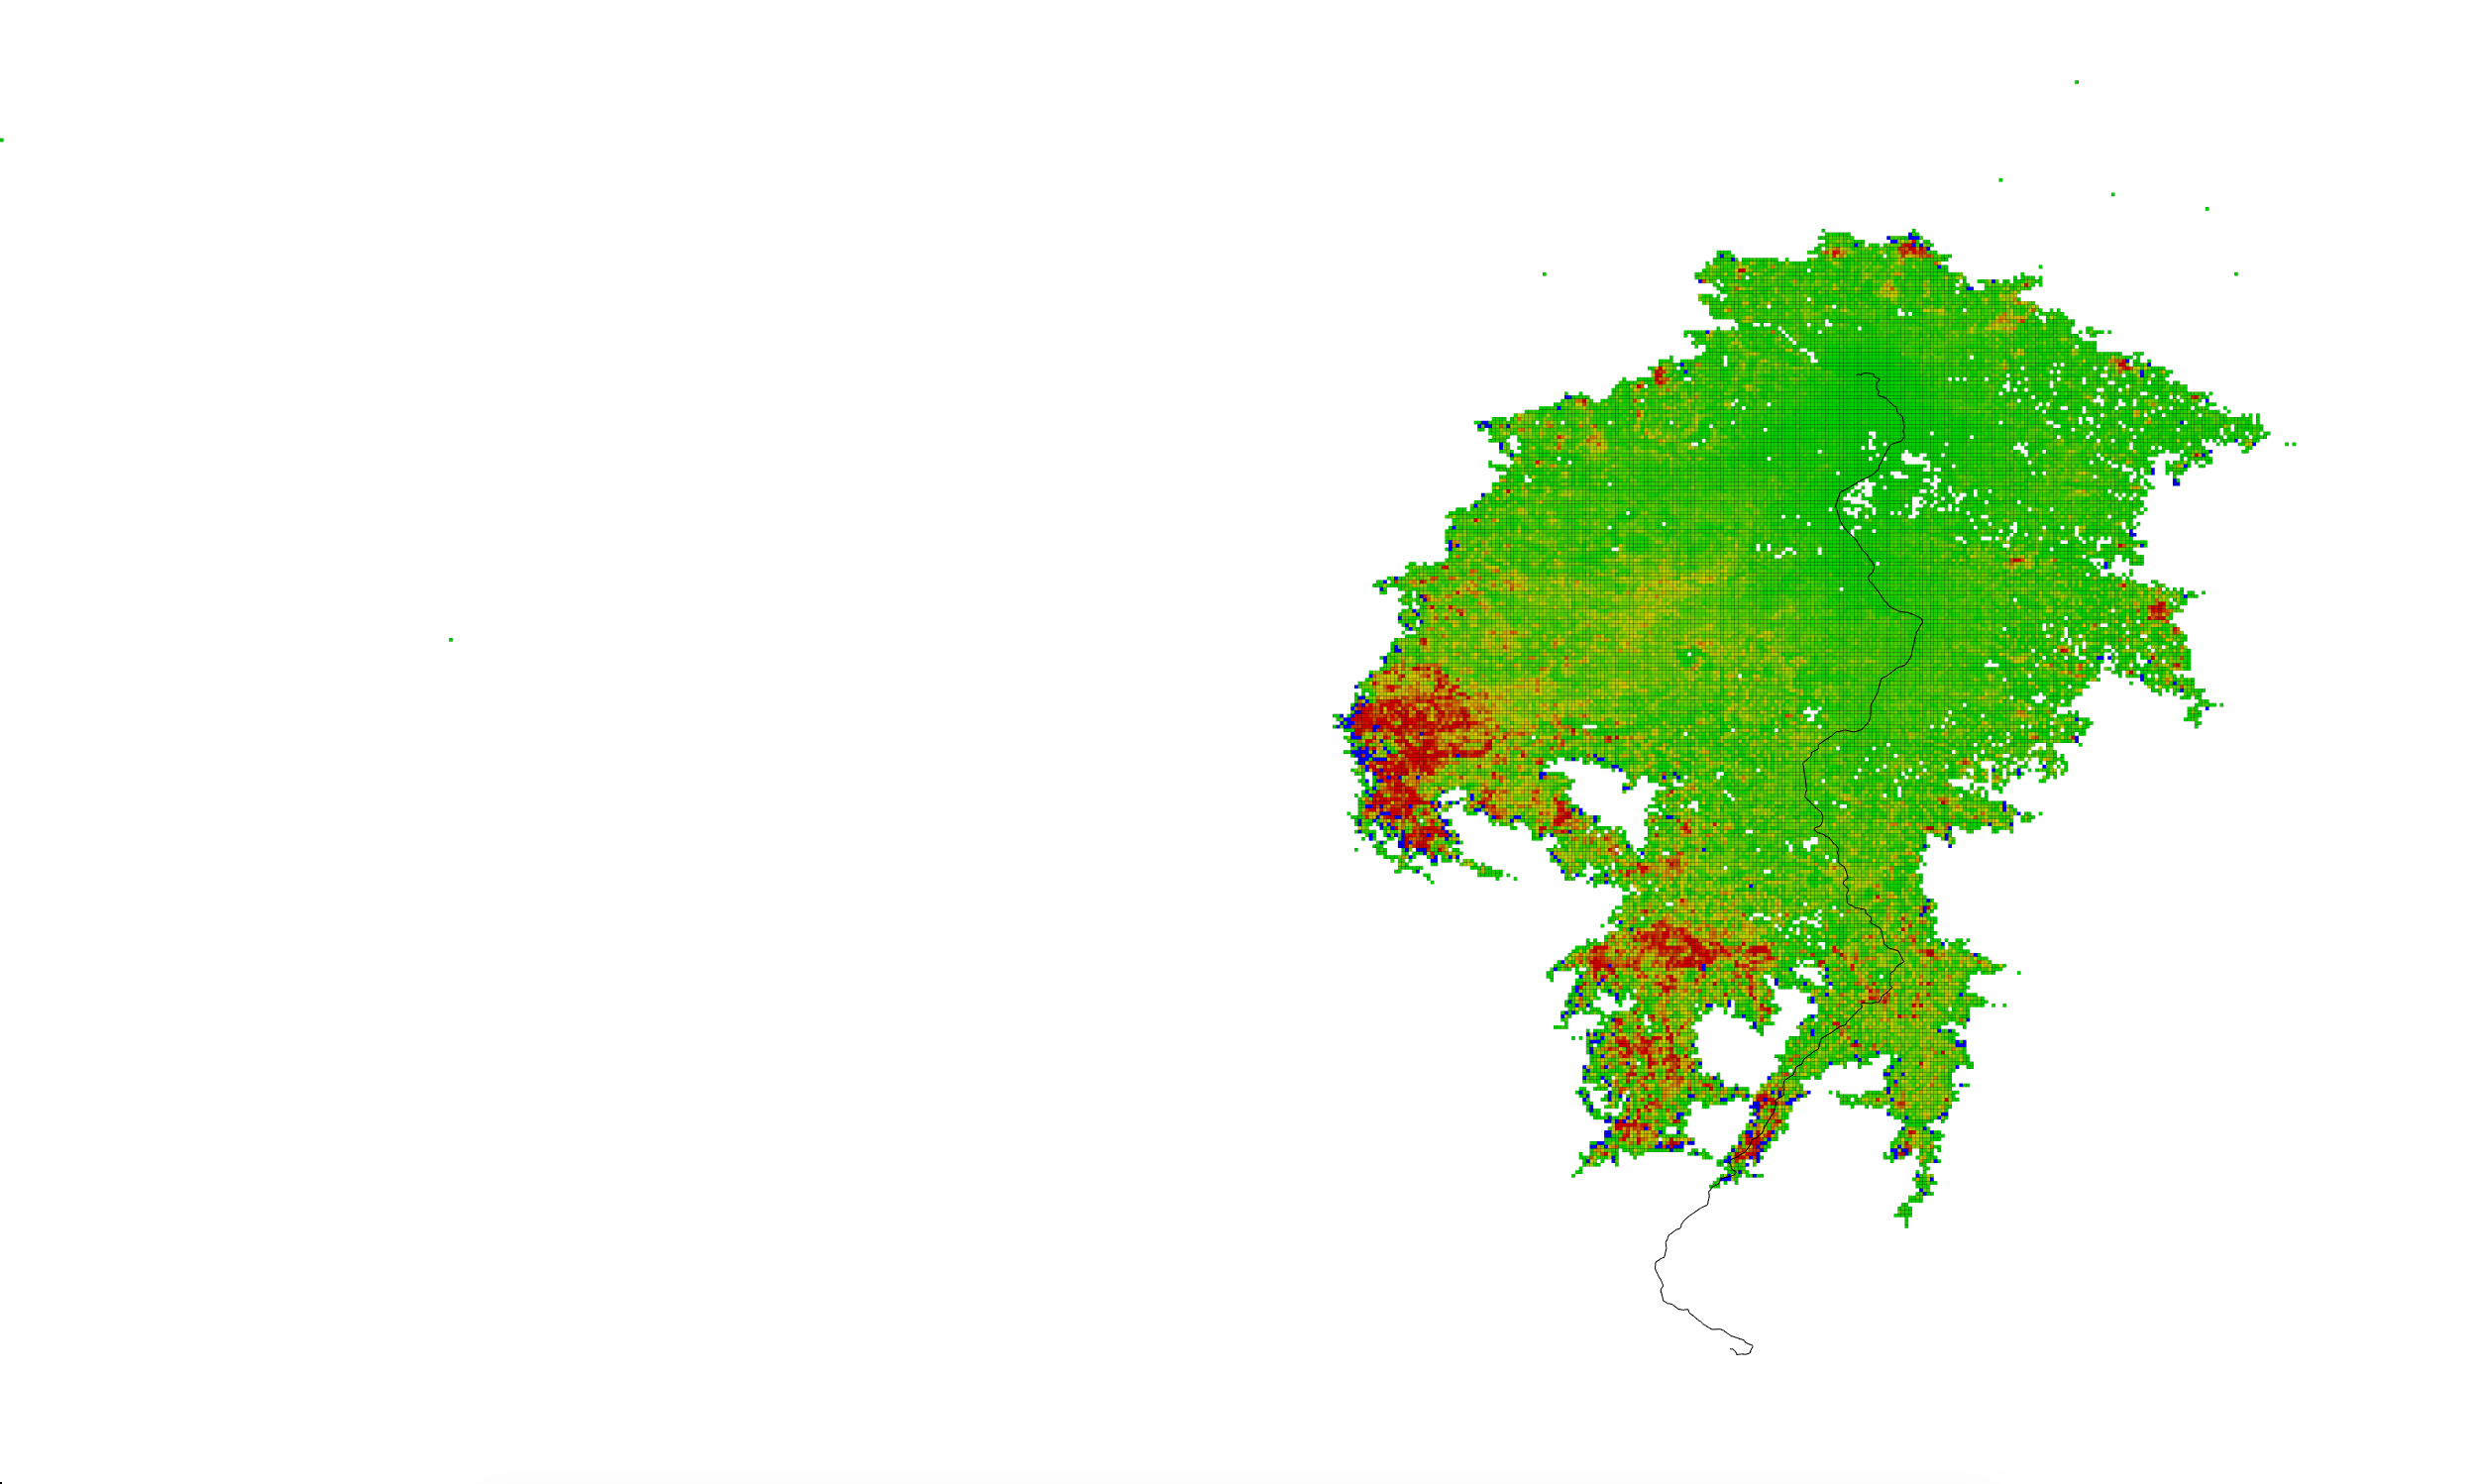
\includegraphics[width=0.5\textwidth]{Images/vis-zoom-small.png}
    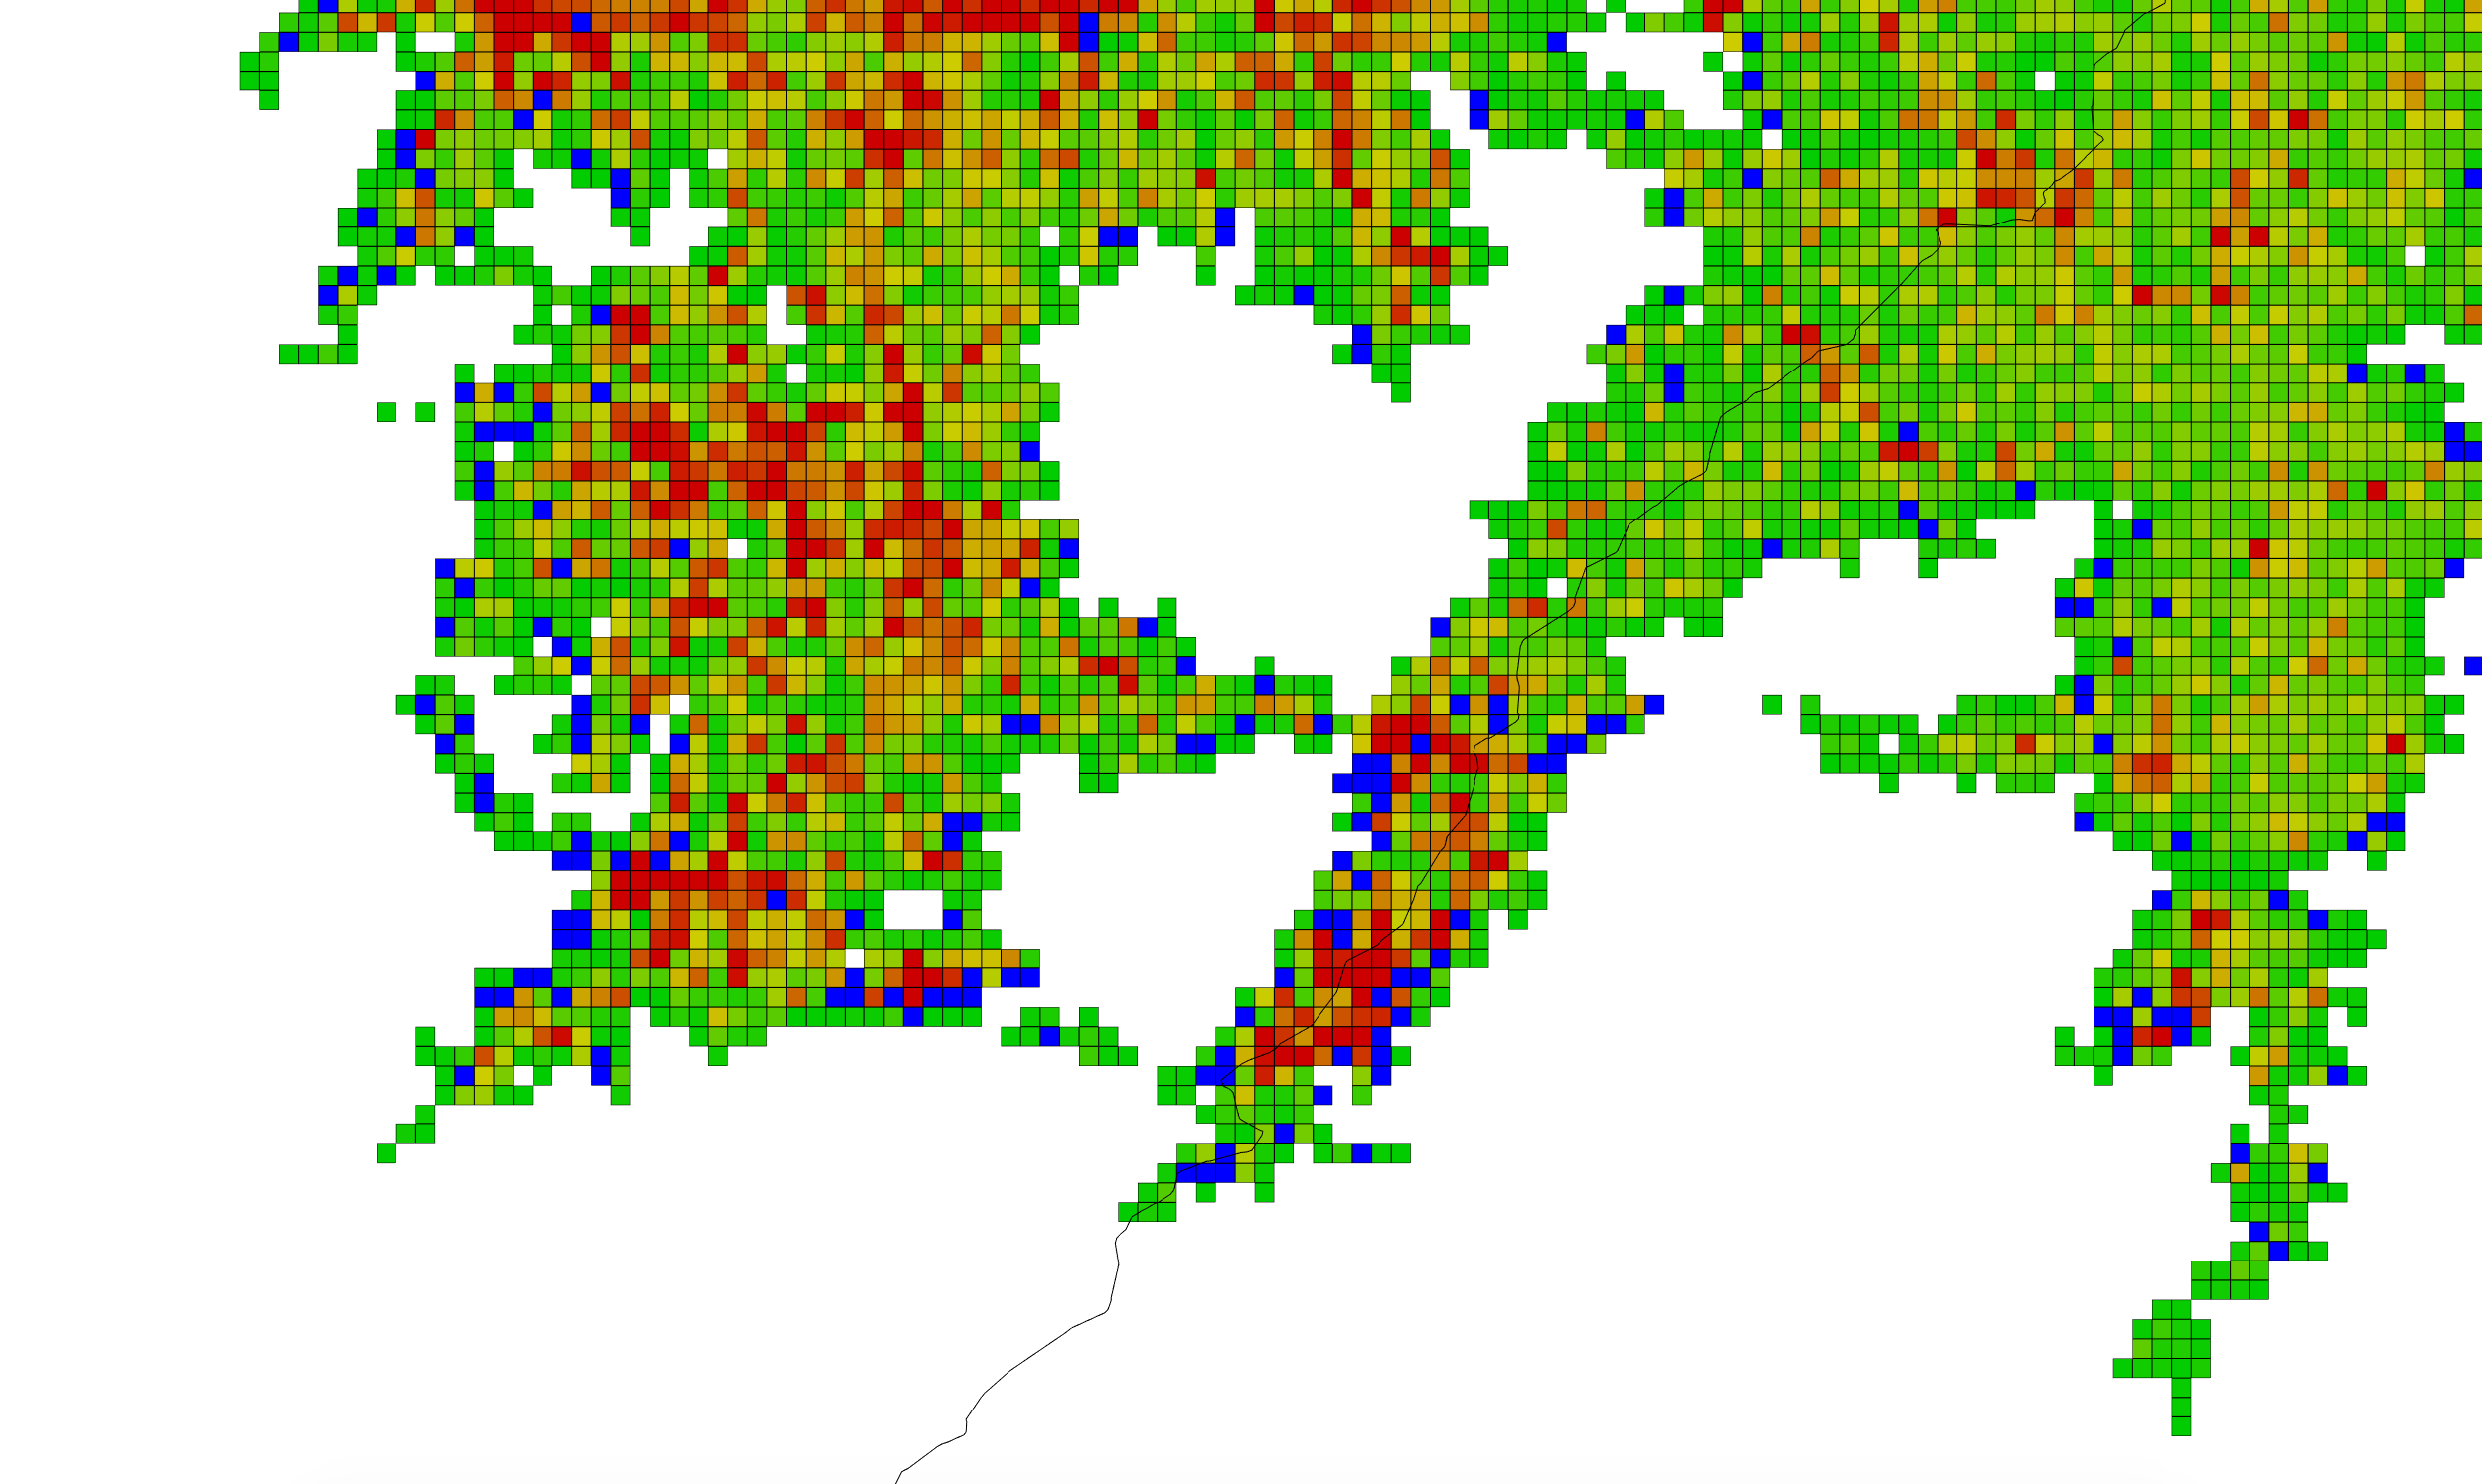
\includegraphics[width=0.5\textwidth]{Images/vis-zoom-large.png}
\caption[]{View on whole graph(left) vz Zoomed view(right)}
\label{fig:zoom}
\end{figure}

We are now able to have a more detailed view on smaller parts of the graph, as can be seen in \Cref{fig:zoom}.

In \Cref{algorithm}, we described the fact that the edges are not recognizable individually on larger routes and we therefore, exluded them from our visualization.
With the new possibility of zooming, showing the edges might become a useful feature for our visualization again.
This could for example be useful, when we want to understand, why specific tiles are loaded much more often than others.
As showing the edges can also make the visualization more confusing and thus distract from the important information, we will make showing the edges optional and make it possible to display an reveal them at any point during the visualization.

\begin{figure}
    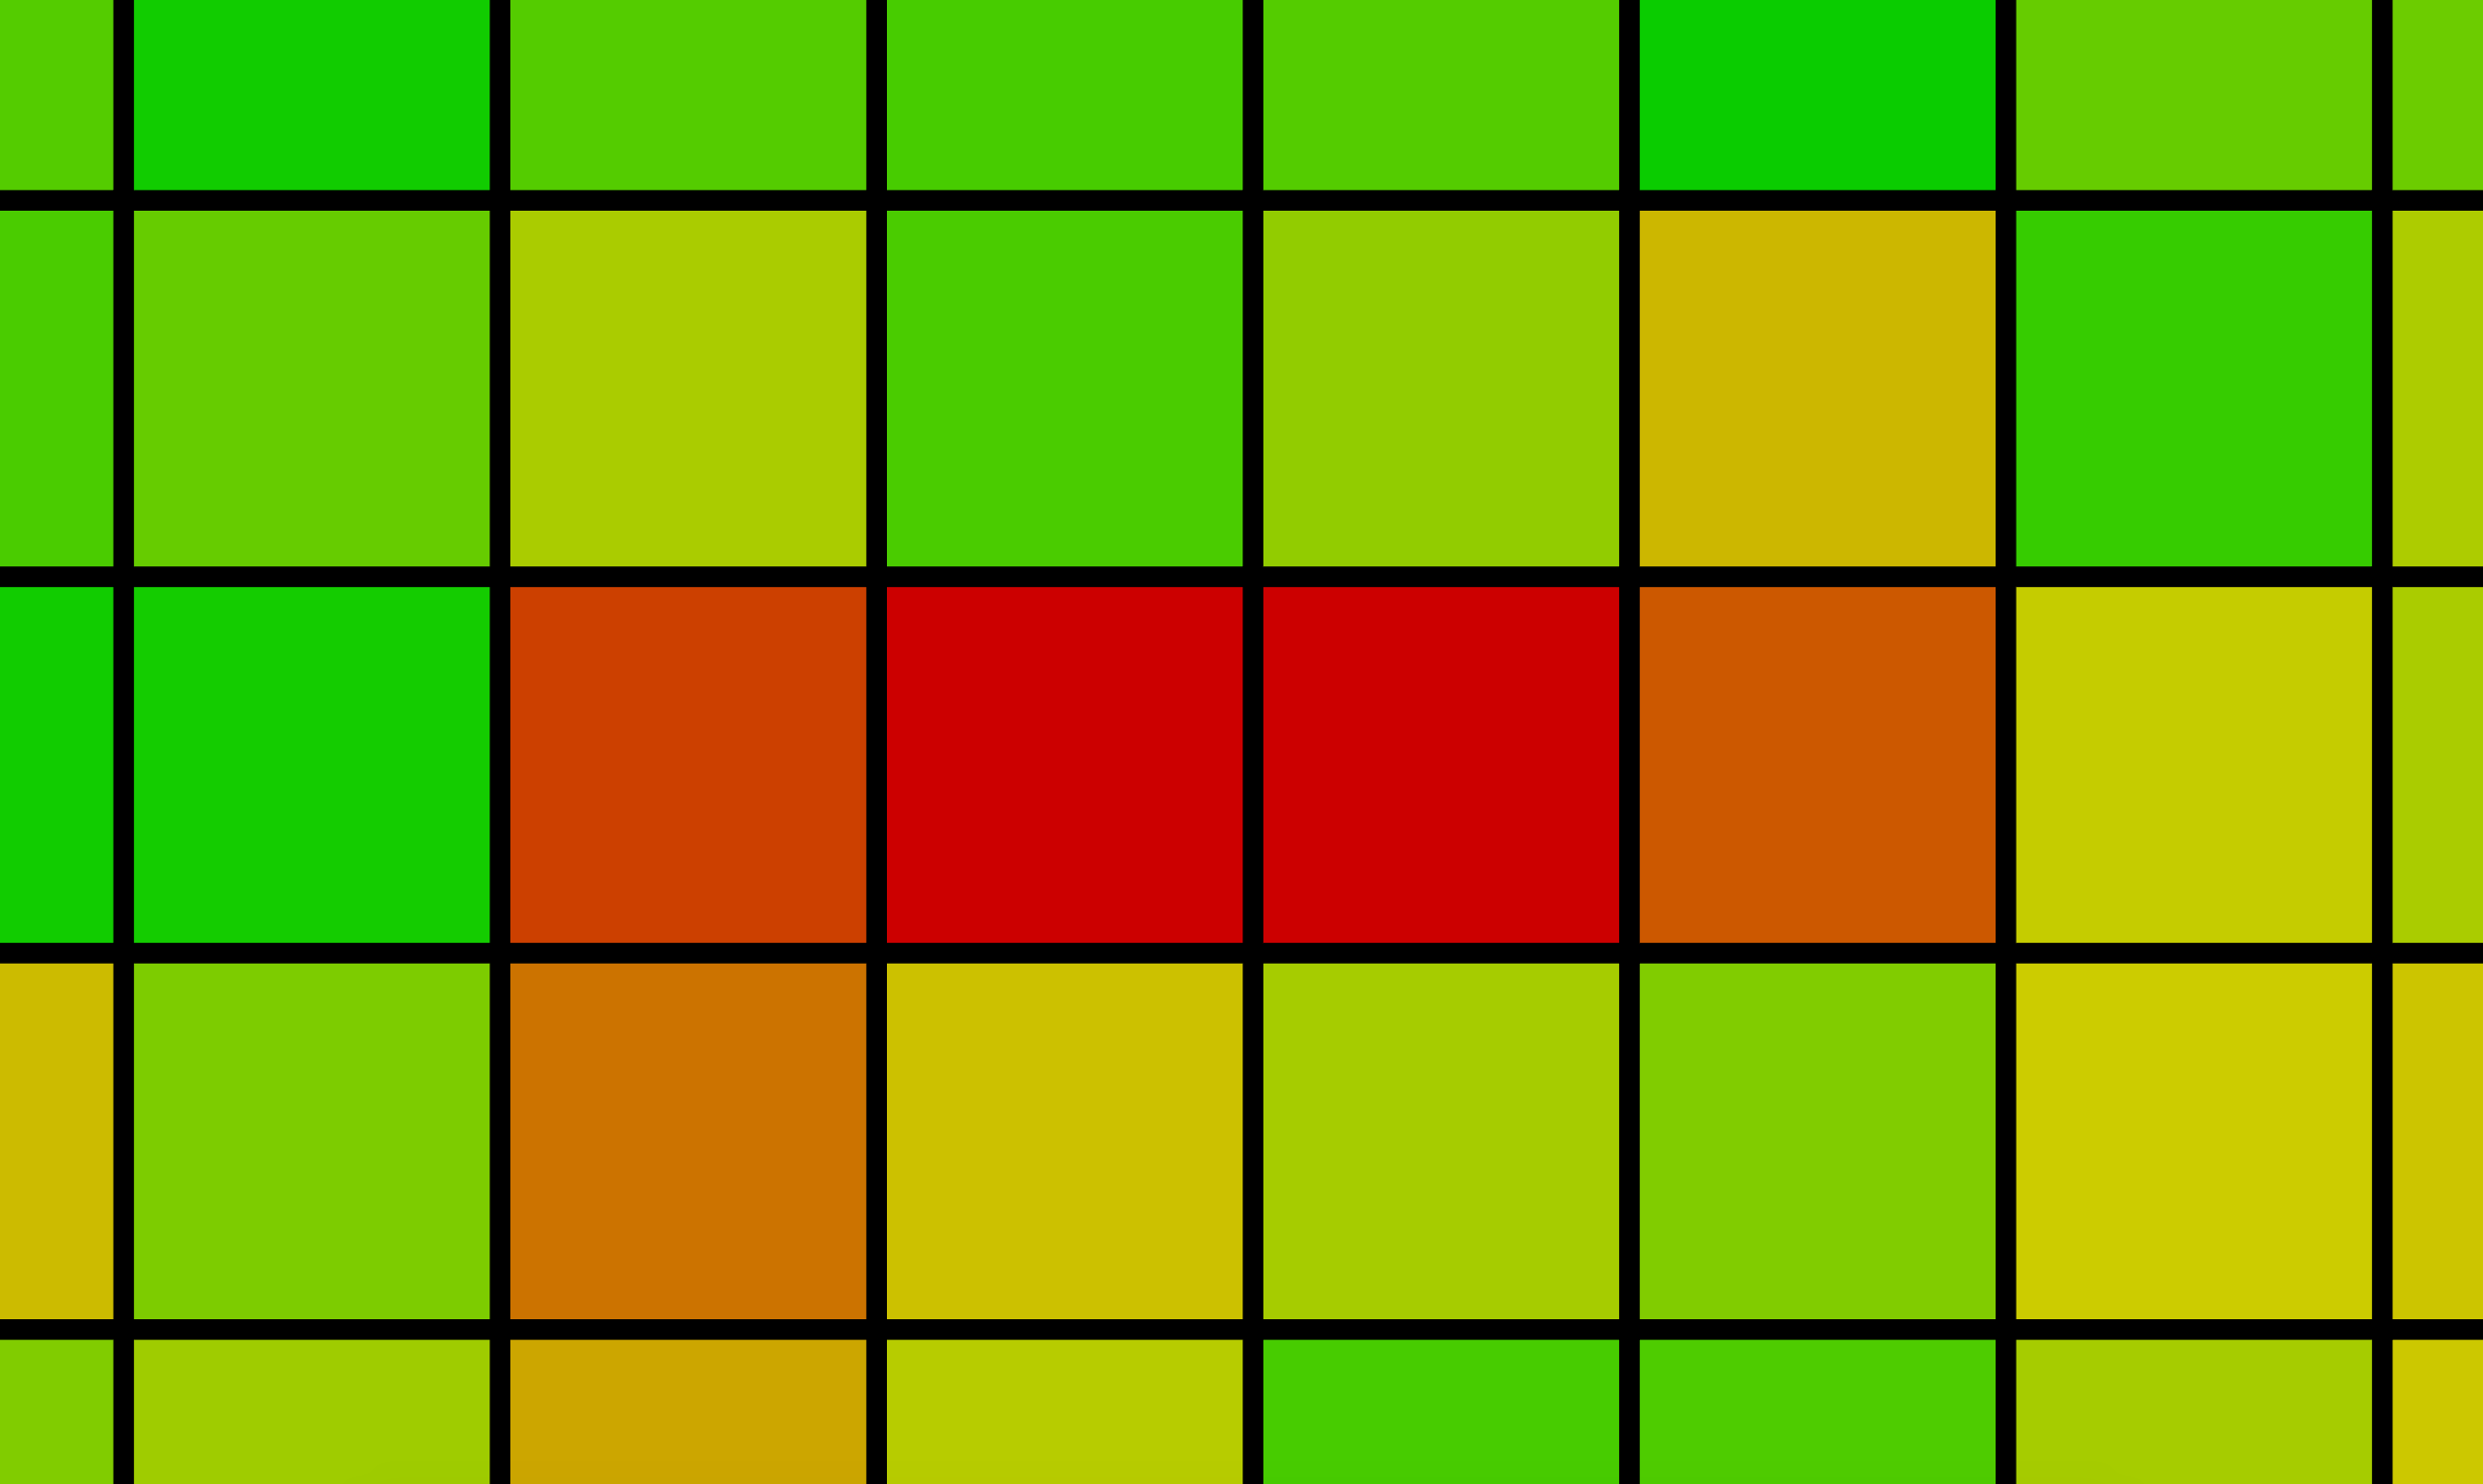
\includegraphics[width=0.5\textwidth]{Images/vis-edges-no.png}
    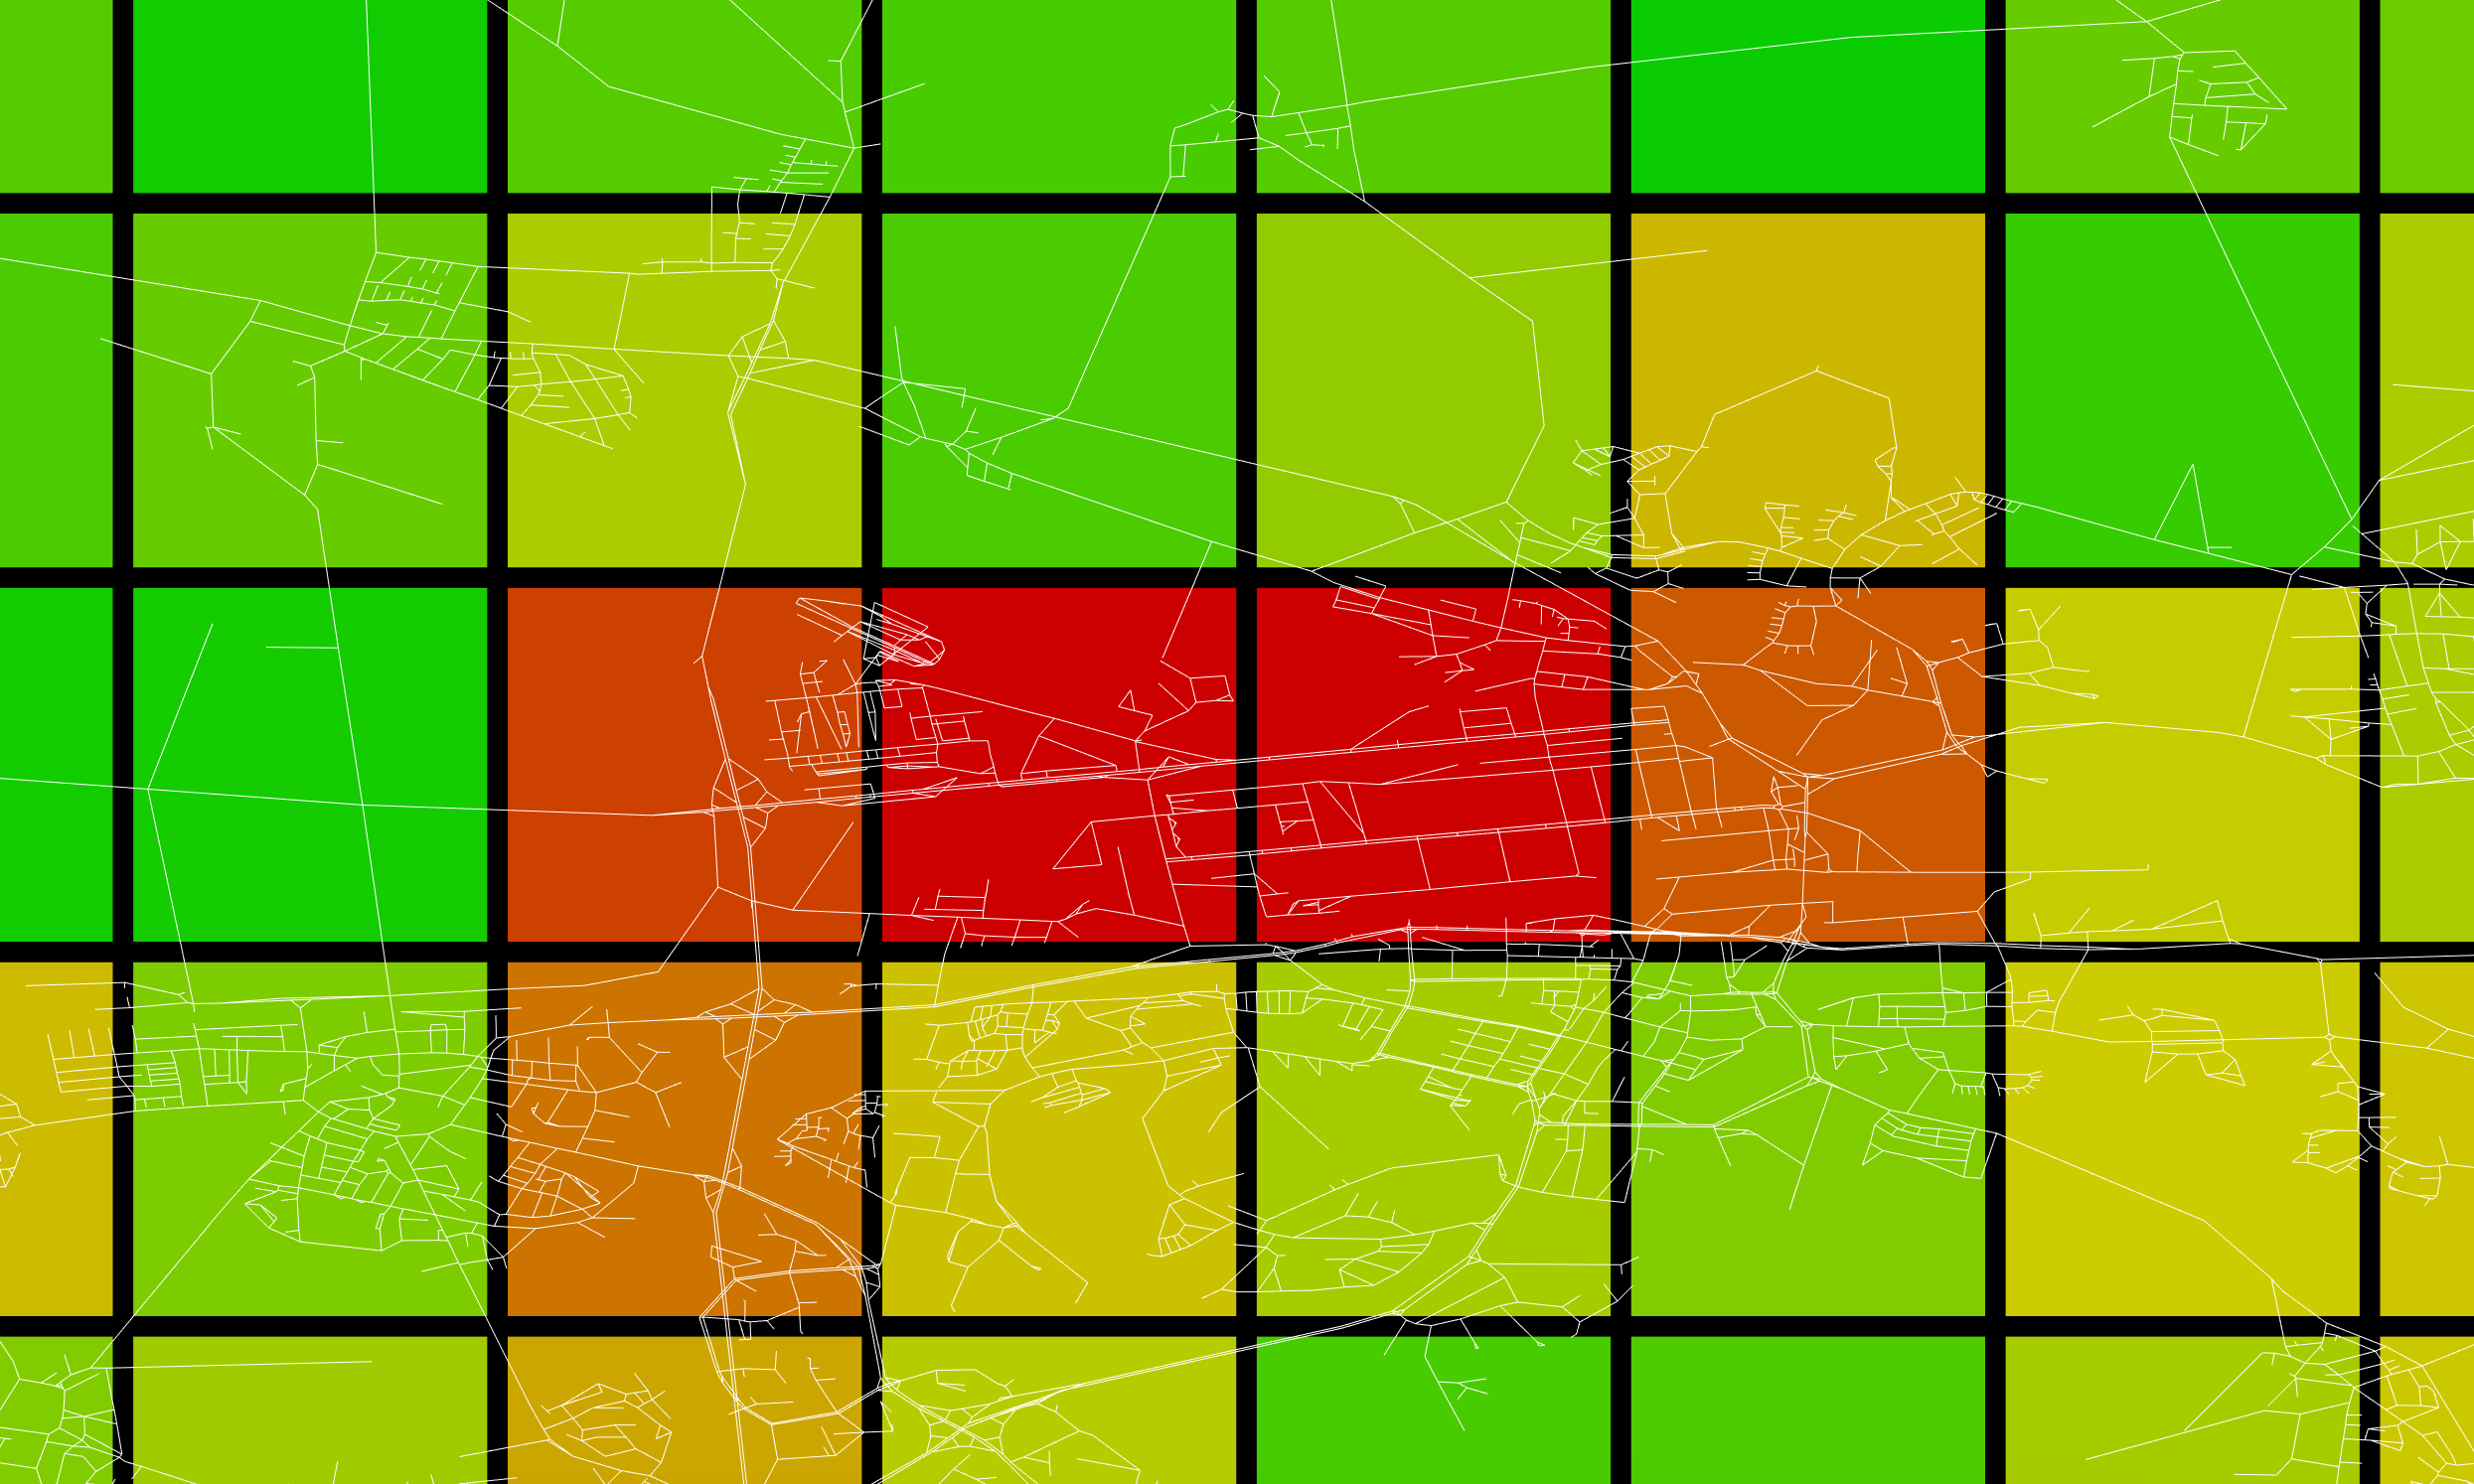
\includegraphics[width=0.5\textwidth]{Images/vis-edges-white.png}
\caption[]{Displaying the edges in addition to the tiles.}
\label{fig:white edges}
\end{figure}

Showing the edges helps to understand why some tiles in \Cref{fig:white edges} are loaded more often than others.
The tiles with more reloadings have an increased level of edges.
Nevertheless, there are also other tiles with many edges, which are loaded less often.
Therefore we decided to use the colored edges described in \Cref{graph} and therefore also include information about their speed.

\begin{figure}
    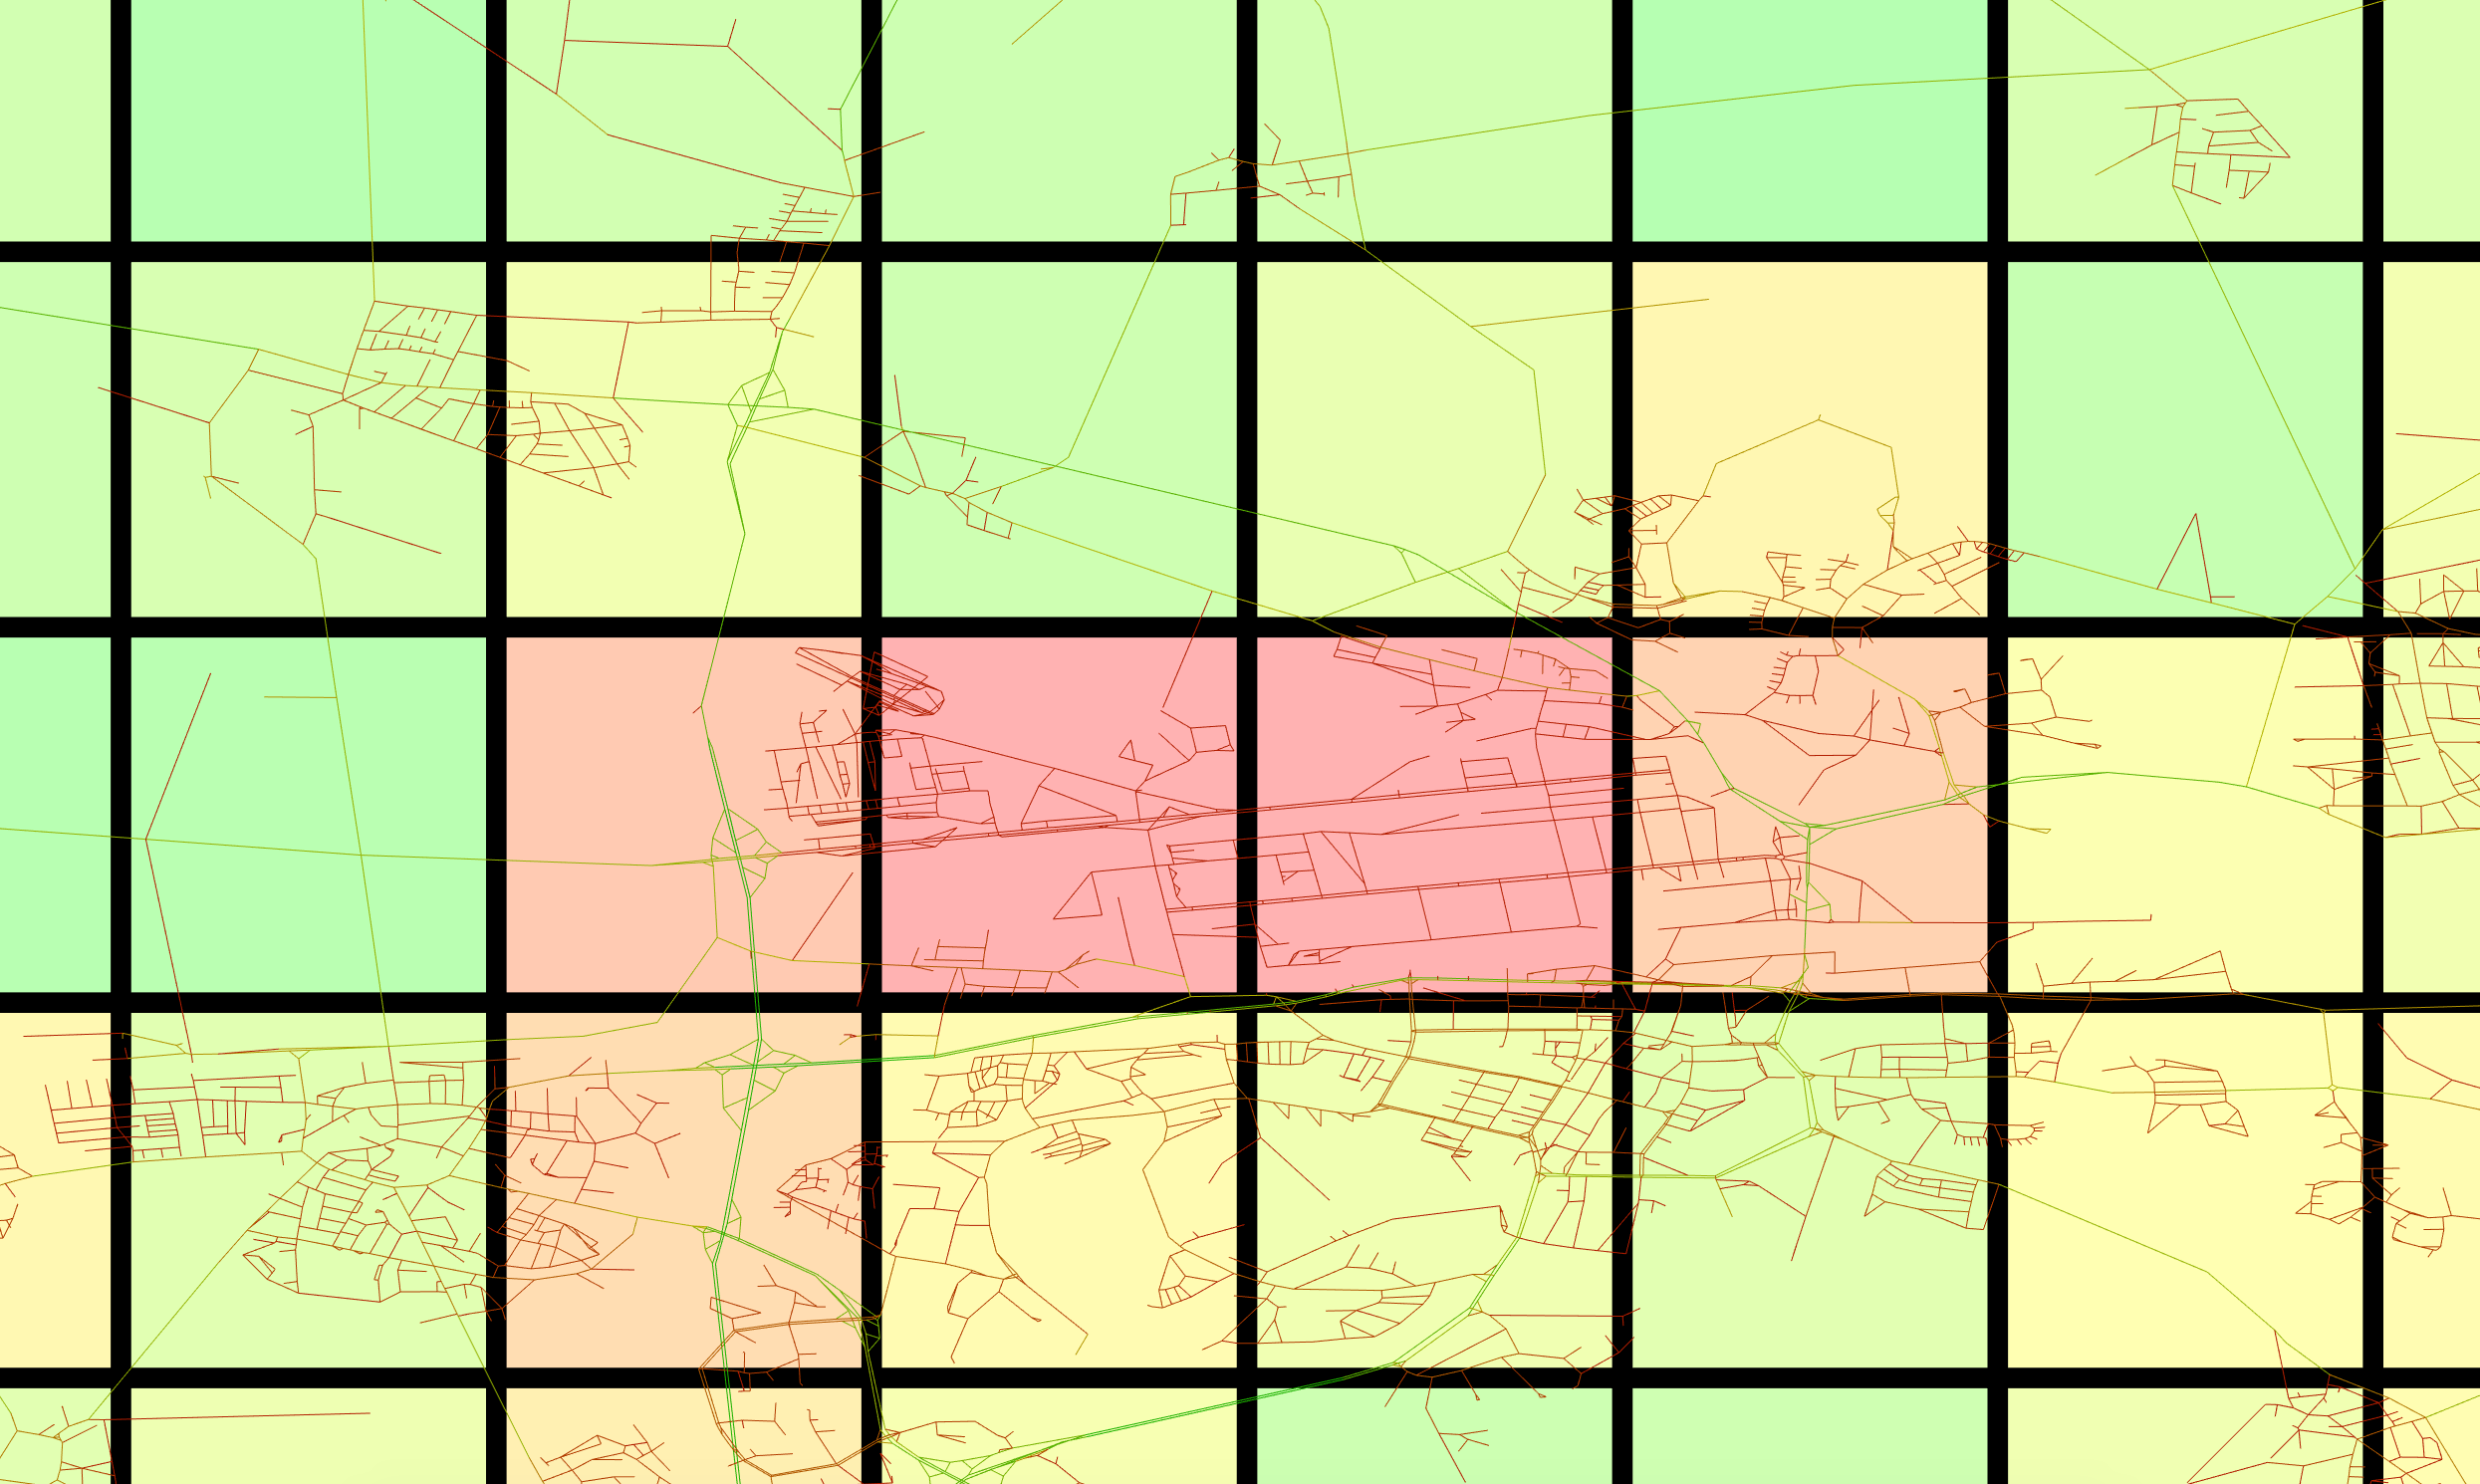
\includegraphics[width=\textwidth]{Images/vis-edges-hsv.png}
\caption[]{Speed based color scheme. For recognizing the edges more clearly the tiles are colored brighter.}
\label{fig:colored edges}
\end{figure}

In \Cref{fig:colored edges} we can now notice that in those tiles that are loaded more often, there are not only many edges, but those with a very low speeds.
Genreally, the surrounding and less loaded tiles allow for higher speeds.

Another feature we needed, after the algorithms improved, was to be able to adjust the level of coloring reloads.
Otherwise it is not possible locate those tiles that have been loaded more often, when considering, that the maximal amount of tile loads is five.
We decided to make this level adjustable while the visualization is running.

\begin{figure}
    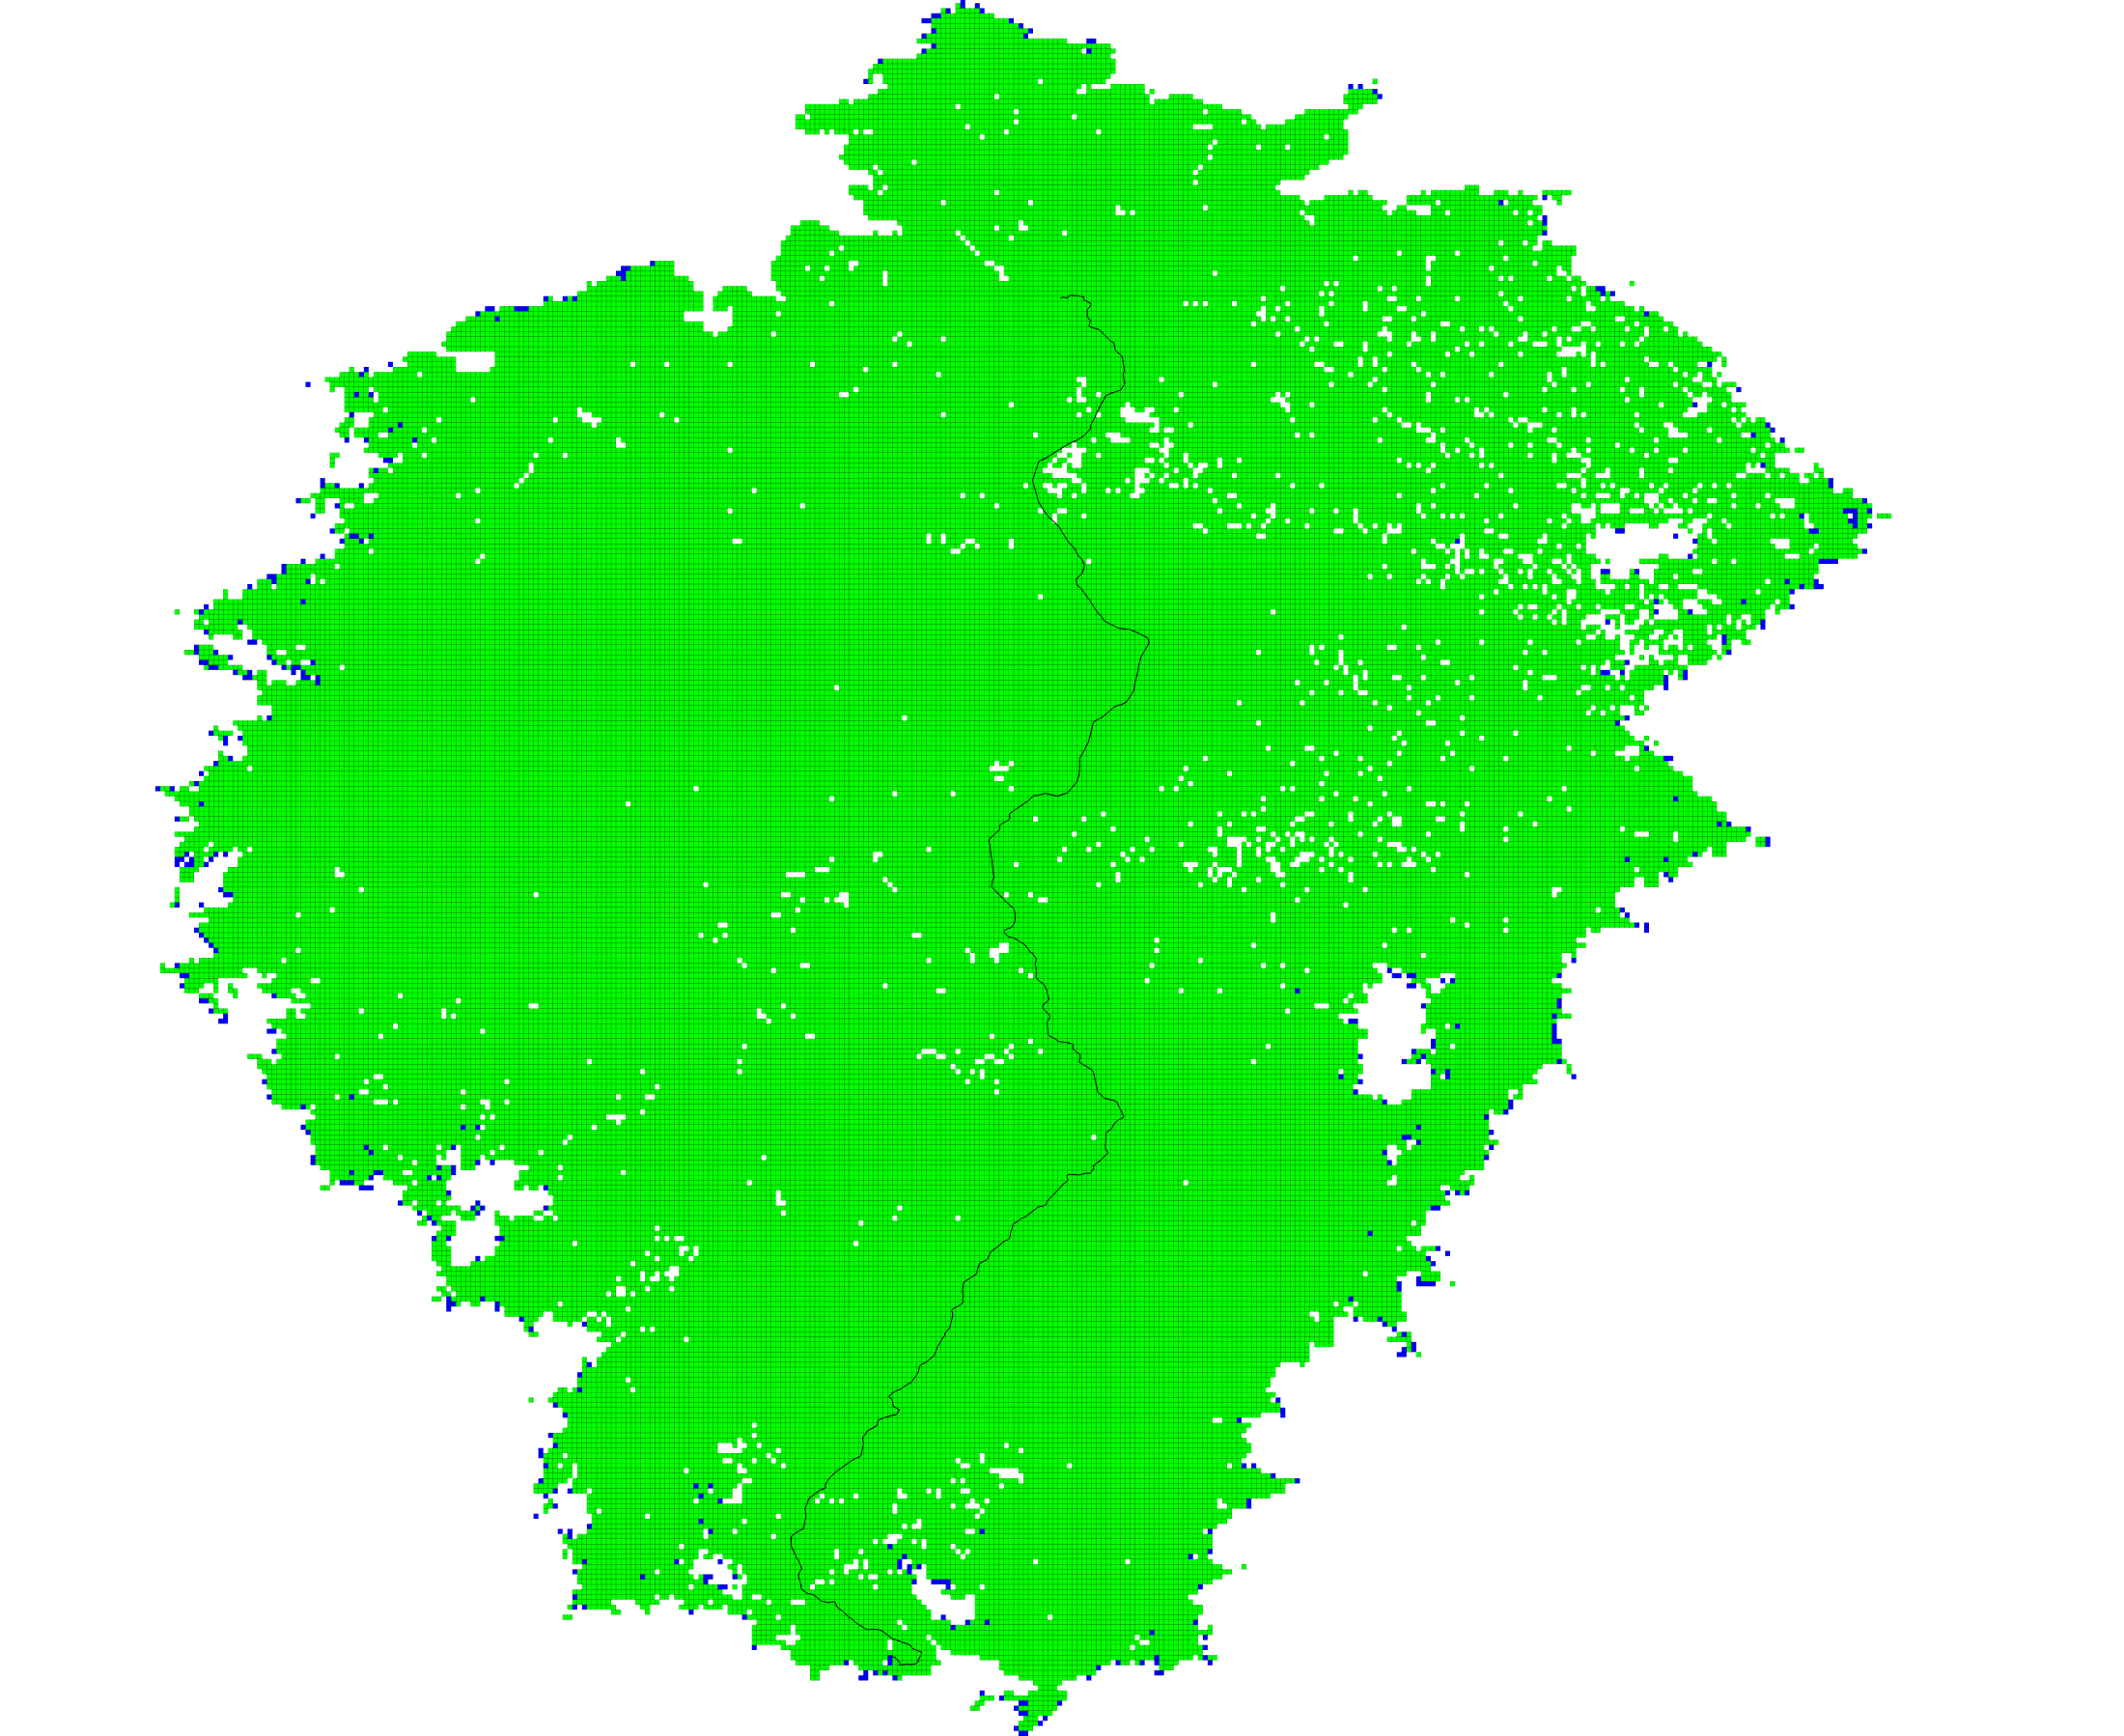
\includegraphics[width=0.5\textwidth]{Images/vis-no-factor.png}
  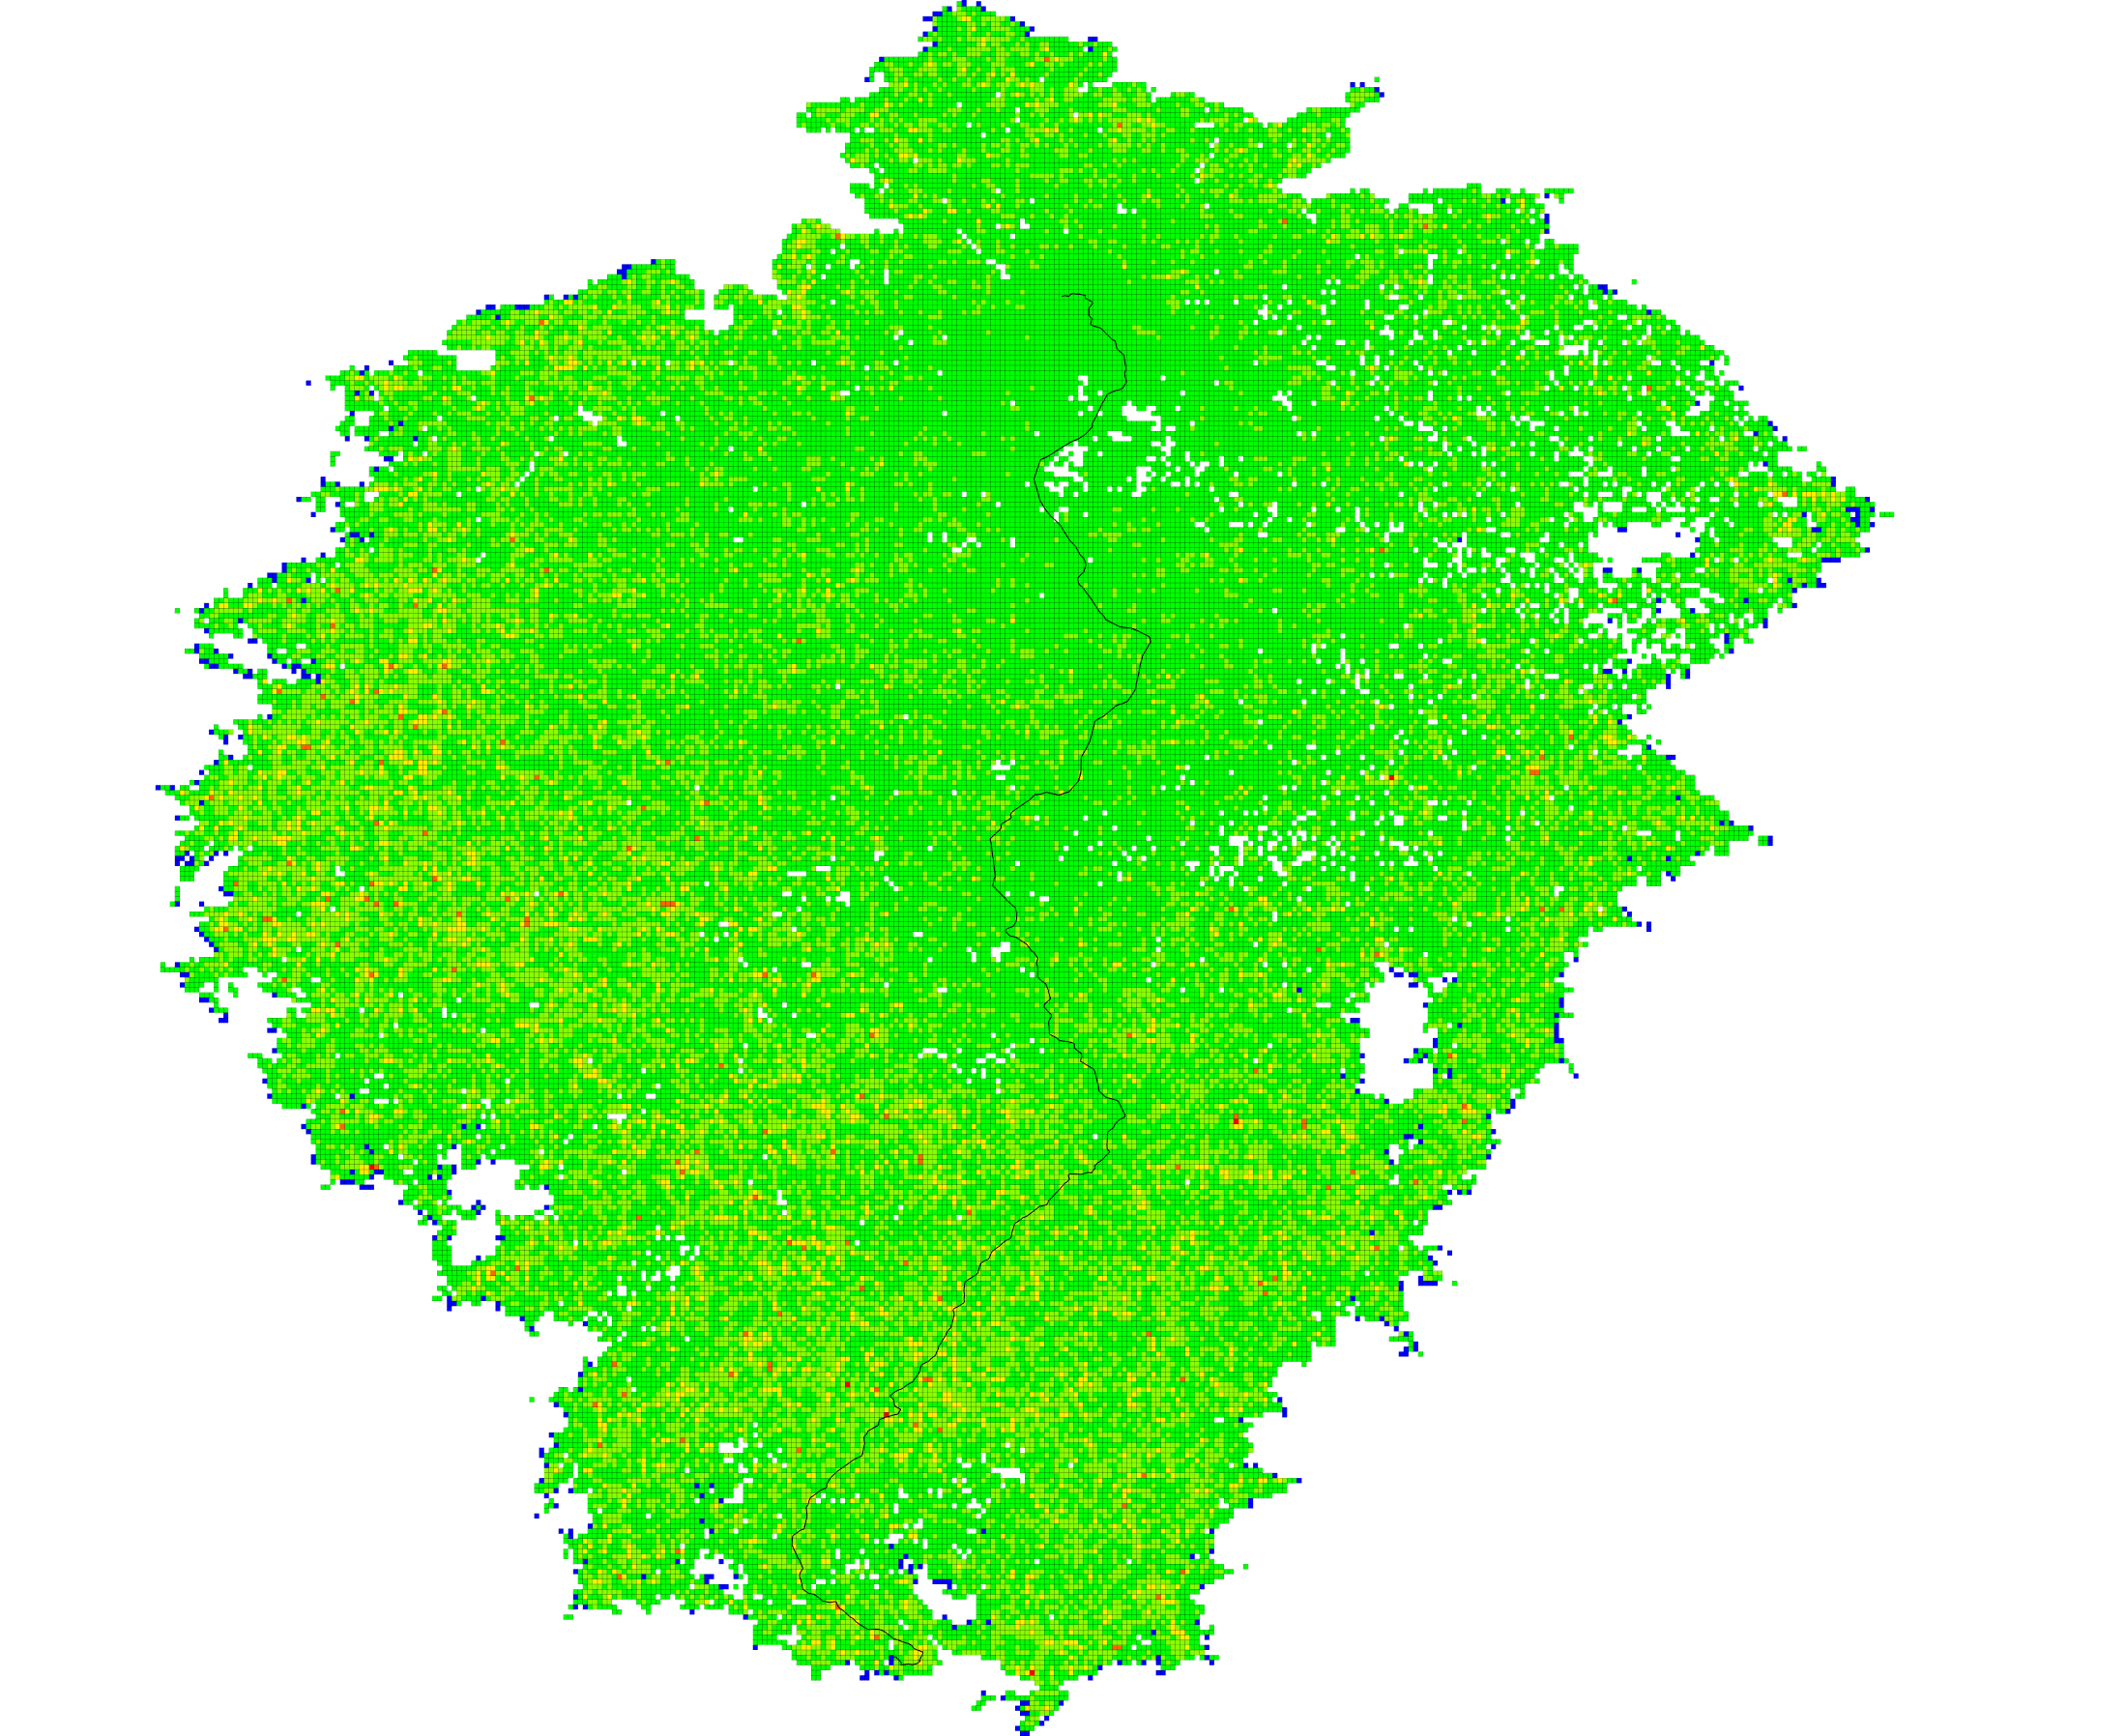
\includegraphics[width=0.5\textwidth]{Images/vis-factor.png}
\caption[]{A well-performing algorithm with normal coloring (left) and a more sensitive coloring (right).}
\label{fig:factor}
\end{figure}

By increasing the coloring of reloads, as can be seen in \Cref{fig:factor}, we are now able to detact weaknesses even on highly developed algorithms.

\chapter{Conclusion} \label{conclusion}

The development of algorithms is a complex process.
Therefore, visualizations can highly improve this process and enable researchers to achieve a better understanding of weaknesses and serve as a basis for discussions.

Due to limited available screen space, the amount of elements that can be displayed without losing comprehensibility is also limited.
Especially on larger routes, this limit raises problems and a certain level of abstraction needs to be found.

Elements need to be assessed with regard to their importance to the class of algorithms and the way the algorithms should be improved.
Another aspect that needs to be considered is the space the elements would require and therefore the number of elements that would have to be displayed.

In our case we decided not to show every single edge as the relation between importance and their amount is disproportionate.
On the contrary the tiles play a major role for the class of algorithms and their total amount is quite low.

The decision as to which elements to show strongly depends on the role of the elements for the class of algorithms.
In our case this decision was quite straightforward, as the most important elements, namely the tiles, were few enough in number, to display.
For algorithms on which stongly represented elements have a strong impact, it might me necessary to introduce an abstraction of those elements.

Having decided which elements to show, it is important to find a way to make the process of the algorithm visible, which we archieved by adding one element after another and coloring the elements accoring to their last usage.
Displaying the result of the algorithm also helped achieving an understanding of the progress of the algorithm.

Finally, we made sure that all information the researchers need is easily accessible.
To this end, we included the cache and added the coloring according to the reloads.
In addition we integrated zooming and panning, showing edges on demand and altering color intensity.
We even created a new visualization for the sole purpose of comparing two algorithms.

\todo{schlusssatz}



% In our case the edges are insofar relevant, as they are a fundermental part of the graph, but for the development of the algorithm they do not play a major role.
% On the other hand the amount of edges is huge.
% Those factors make those methods that use the edges for showing the process of the algorithm less sensemaking because of their lack of clairity.
% Nevertheless in combination with the zoom feature displaying edges becomes reasonable, as zooming in reduces the amount of displayed elements on the screen and therefore enables a more detailed view.
%
% On the contrary the total amount of tiles is in a reasonable relation to their importance for the algorithm.
% In addition the rectangular representation of the tiles turned out to be a good canvas for presenting information about the cache and the performance of the displayed algorithm.

%\begin{itemize}
%     \item verschiedene Projektionen
%     \item different layers
%     \item gerichtete edges
% \end{itemize}

% References
\renewcommand*{\bibname}{References}
\bibliographystyle{abbrvnat}
\bibliography{Files/References}


\chapter*{Independence Declaration}
\addcontentsline{toc}{chapter}{Declaration of Authorship}
\thispagestyle{empty}

I hereby declare that the thesis submitted is my own unaided work. All direct or indirect sources used are acknowledged as references.\vspace{2 ex}

Potsdam, \today\\[6 ex]

\begin{flushleft}
    \begin{tabular}{p{5cm}}
        \hline
        \centering\footnotesize\printAuthor
    \end{tabular}
\end{flushleft}


\end{document}
